\documentclass[11pt,fleqn,x11names,table]{book}                                                  
% Dimensiones y m�rgenes=1 pulgada alrededor del texto

     
\usepackage[margin=1in]{geometry}
\usepackage[mathscr]{euscript}
%----------------------------------------------------------------------
%--------------------------------------------------------------------------
% PAQUETES Y ESTILO 
%--------------------------------------------------------------------------
% Paquetes 
\usepackage[spanish]{babel}
%\usepackage[latin1]{inputenc}                      % Entrada de acentos
\usepackage[T1]{fontenc}
\usepackage[utf8]{inputenc}
\usepackage[autostyle, spanish = mexican]{csquotes}% manejo de comillas: " "
\MakeOuterQuote{"}
\usepackage{pslatex}         
                     % Fuentes finas postscript
%\usepackage[sc]{mathpazo}                         % Fuentes mathpazo
%\usepackage[condensed,math]{kurier}
%\usepackage{palatino}
%\usepackage{librecaslon}
%\usepackage{rec-thy}

\usepackage{helvet}
\linespread{1.05}                                  % Fuente Palatino necesita espaciado
\usepackage[full]{textcomp}                        % Caracteres especiales como ' (recto)
\usepackage{xcolor}                                % Color: X11names (en el documentclass)

% COLORES personales---------------------------------------------------
    \definecolor{colortitulo}{RGB}{11,17,79} % Titulo
    \definecolor{colordominante}{RGB}{68,82,115} %Color del Cuadro grannde
    \definecolor{colordominanteF}{RGB}{219,68,14}
    \definecolor{colordominanteD}{RGB}{137,46,55}
    \definecolor{mostaza}{RGB}{231,196,25}
    \definecolor{amarilloM}{RGB}{248,199,90}
    \definecolor{amarilloD}{RGB}{251,237,121}
    \definecolor{azulF}{RGB}{66,74,86}
    \definecolor{grisD}{rgb}{.3,.3,.3}
    \definecolor{grisF}{rgb}{.6,.6,.6}
    \definecolor{grisamarillo}{RGB}{248,248,245} 
    \definecolor{miverde}{RGB}{44,162,67}
    \definecolor{verdep}{RGB}{94,142,118}
    \definecolor{verdencabezado}{RGB}{220,220,220} %Color de rect�ngulo de encabezado
    \definecolor{verdeF}{RGB}{5,92,8}
    \colorlet{mygray}{black!20}
    \newcommand{\verde}{\color{miverde}}
    
 
    
% Fin COLORES personales-------------------------------------------------

%---------------------------------------------------------------Colores 1
%\definecolor{colortitulo}{RGB}{219,68,14} %
%\definecolor{colordominante}{RGB}{243,102,25}
%\definecolor{colordominanteF}{RGB}{219,68,14}
%\definecolor{colordominanteD}{RGB}{137,46,55}
%\definecolor{mostaza}{RGB}{231,196,25}
%\definecolor{amarilloM}{RGB}{248,199,90}
%\definecolor{amarilloD}{RGB}{251,237,121}
%\definecolor{grisamarillo}{RGB}{248,248,245}
%\definecolor{miverde}{RGB}{44,162,67}
%\definecolor{verdep}{RGB}{94,142,118}
%\definecolor{verdencabezado}{RGB}{220,220,220} %Color de rect�ngulo de encabezado
%\definecolor{verdeF}{RGB}{5,92,8}
%\colorlet{mygray}{black!20}
%\definecolor{azulF}{rgb}{.0,.0,.3}
%\definecolor{grisD}{rgb}{.3,.3,.3}
%\definecolor{grisF}{rgb}{.6,.6,.6}
%\definecolor{miverde}{RGB}{44,162,67}
%\renewcommand{\verde}{\color{miverde}}
%---------------------------------------------------------------Colores 2



%\usepackage{psboxit}
\usepackage{pstricks}
\usepackage{xparse}
\usepackage{tcolorbox} 
\tcbuselibrary{skins,breakable}  % Librer�as tcolorbox
\usepackage{tikz,tkz-tab} % Cajas de Teoremas, ejemplos, etc.
\usetikzlibrary{positioning,shadows,backgrounds,calc}%
\usepackage{tikzpagenodes}
\usepackage{xargs}  % Comandos con opciones
\DeclareGraphicsExtensions{.pdf,.png,.jpg}
\usepackage{multicol}
% %\usepackage{epstopdf}% Conversi�n - Miktes 2.9 o inferior, TexLive 2009. o inferior
\usepackage[small,bf]{caption}
\usepackage[breaklinks,colorlinks=true, pdfstartview=FitV, linkcolor=azulF, citecolor=azulF, urlcolor=azulF]{hyperref}
\usepackage{exscale,amsmath,amssymb,amsfonts,latexsym,cancel,stmaryrd}
\usepackage[ruled,,vlined,lined,linesnumbered,algochapter]{algorithm2e}
\usepackage{framed}
\usepackage{titletoc}
\usepackage{calc}
\usepackage{colortbl} 
\usepackage{tabularx}
\usepackage{fancyvrb}
%\usepackage{minted}   %habilitar solo en Ubuntu (Linux)
\usepackage{array}
\usepackage{wasysym}
\usepackage{supertabular}
\usepackage{booktabs}
\usepackage[shortlabels]{enumitem}
%\usepackage{mathrsfs}
\usepackage{calrsfs}
\usepackage{wrapfig}%Figuras al lado de texto
\usepackage[lflt]{floatflt} %Figuras flotantes entre el texto
\usepackage{parskip} %Quita la sangría al iniciar los párrafos



%----------------------------------------------------------------------------------------
% Fuentes
%----------------------------------------------------------------------------------------
% Comandos para fuentes especiales
\newcommandx*{\fnte}[4][1=pag,2=9,3=n]{{\color{azulF}\fontfamily{#1}
\fontsize{#2}{1}\fontshape{#3}\selectfont{#4}}}

\newcommandx*{\fntb}[4][1=pag,2=9,3=n]{{\color{azulF}\fontfamily{#1}\fontsize{#2}{1}\fontseries{b}\fontshape{#3}\selectfont{#4}}}

\newcommandx*{\fntg}[4][1=pag,2=9,3=n]{{\color{grisF}\fontfamily{#1}\fontsize{#2}{1}\fontshape{#3}\selectfont{#4}}}

\newcommand{\fhv}[2]{{\fontfamily{pag}\fontsize{#1}{1}\selectfont{#2}}}

\newcommand{\fhvb}[2]{{\textcolor[RGB]{68,82,115}{\fontfamily{pag}\fontseries{b}\fontsize{#1}{1}\selectfont{#2}}}}
% Fin fuentes----------------------------------------------------------

%*************************************** DISEÑO *****************************************

%----------------------------------------------------------------------------------------
% Cabeceras
%----------------------------------------------------------------------------------------
\usepackage{fancyhdr}

% N�meros de p�gina en rect�ngulos y cap�tulo. 
\usepackage[absolute]{textpos}
    \setlength{\TPHorizModule}{10mm}% 1 generic horizontal unit is equivalent to 10mm
    \setlength{\TPVertModule}{10mm}% 1 generic vertical unit is equivalent to 10mm
    \textblockorigin{0mm}{0mm}% top left corner set as origin

%------------------------------------------------------------------------------
% Decoraci�n de cabeceras 
% Texto en secciones
\newcommand{\helvb}{%
\fontfamily{phv}\fontseries{b}\fontsize{9}{11}\selectfont}
\newcommand{\helv}{%
\fontfamily{phv}\fontsize{9}{11}\selectfont}
\renewcommand{\sectionmark}[1]{\markright{\thesection\hspace{5pt}#1}{}} 
% Configuraci�n de fuentes para el n�mero de p�gina en el encabezado
\fancyhf{} 
%OP 1: Todas las p�ginas con la secci�n a la izquierda
%\fancyhead[LO,LE]{\rightmark} % L=Left, O=Odd y  E=Even pages
%OP 2: Todas las p�ginas con la secci�n a la izquierda en un rect�ngulo (todo el header)

%Rect�ngulo en el encabezado
\fancyhead[LO,LE]{\helv\rightmark
\begin{textblock}{1}(0,0)
\begin{tikzpicture}[remember picture,overlay]
  %\fill[grisamarillo] (current page.north west) 
  \fill[verdencabezado,opacity=50] (current page.north west) %color del encabezado
  rectangle
  ([xshift=2pt,yshift=-3pt]current page.east|-current page header area.south east);
\end{tikzpicture}
\end{textblock}
}
% Fin decoraci�n cabeceras

\renewcommand{\headrulewidth}{0pt}   % Ancho de la l�nea bajo el encabezado
\addtolength{\headheight}{2.5pt}     % Aumente el espacio alrededor de la cabecera 
\renewcommand{\footrulewidth}{0pt}   % Elimina la l�nea en el pie de p�gina
% Estilo para cuando se especifica "pagestyle plain"
\fancypagestyle{plain}{\fancyhead{}\renewcommand{\headrulewidth}{0pt}} 

% Elimina el encabezado de las p�ginas impares vac�as al final de los cap�tulos
\makeatletter
\renewcommand{\cleardoublepage}{
\clearpage\ifodd\c@page\else
\hbox{}
\vspace*{\fill}
\thispagestyle{empty}
\newpage
\fi}
\makeatother

% N�meros de p�gina en el borde
\fancyfoot[LO]{
\begin{textblock}{3}(21,1) % y=1 inch = margen
\begin{tikzpicture}[overlay]
\node[draw=colordominante,
rectangle,minimum width=2cm, minimum height=2cm,
anchor=west,
fill=colordominante,font=\fontsize{25}{1}\sffamily\bfseries,inner sep=2pt,outer sep=2pt] 
at (-1.5cm,0pt){\textcolor{gray!10}{\thepage}};
\end{tikzpicture}
\end{textblock}
}

\fancyfoot[RE]{
\begin{textblock}{3}(18,1)% y=1 inch = margen
\begin{tikzpicture}[overlay]
\node[draw=colordominante,
rectangle,minimum width=2cm, minimum height=2cm,
anchor=west,
fill=colordominante,font=\fontsize{25}{1}\sffamily\bfseries,inner sep=2pt,outer sep=2pt] 
at (-1.5cm,0pt){\textcolor{gray!10}{\thepage}};   
\end{tikzpicture}
\end{textblock}
}
%-- Fin cabeceras 

%----------------------------------------------------------------------------------------
% Color en los m�rgenes
%----------------------------------------------------------------------------------------
% \pagecolor{grisamarillo}
% \usepackage{eso-pic}
% \pagecolor{grisamarillo}
% \AddToShipoutPictureBG{%
%  \AtTextLowerLeft{\color{grisamarillo}%
%   \rule[-\footskip]{\textwidth}{\dimexpr\textheight+\footskip}}}

% Fin color m�rgenes



%----------------------------------------------------------------------------------------
% Pr�logo
%----------------------------------------------------------------------------------------
\NewDocumentEnvironment{prologo}{O{}}{%
\addcontentsline{toc}{schapter}{%
\hspace{6em}{\color{azulF}{\fontfamily{phv}\fontsize{9}{10}\selectfont Pr\'ologo}} \qquad}
\chapter*{Pr�logo}
\smallskip\smallskip
\begin{minipage}{0.9\textwidth}
 #1}{\end{minipage}}
 

%----------------------------------------------------------------------------------------
% T�tulo (PORTADA)
%----------------------------------------------------------------------------------------


\newcommand*{\titulo}[4]{\begingroup%
\raggedleft 
\vspace*{\baselineskip} % Espacio en blanco en la parte superior de la p�gina
\renewcommand{\headrulewidth}{2pt}

\thispagestyle{empty}

\begin{minipage}[c][0.15\textheight][c]{0.2\textwidth}
	\begin{center}
		
\includegraphics[width=2cm, height=2cm]{images/logoF.jpeg}
	\end{center}
\end{minipage}
\begin{minipage}[c][0.15\textheight][t]{0.75\textwidth}
	\begin{center}
		\vspace{.9cm}
		{\scshape \bf \Large \color{azulF}Universidad Nacional Aut\'onoma de M\'exico}
		\vspace{.3cm}
		\textcolor[RGB]{191,191,191}{\hrule height2.5pt}
		\vspace{1.5mm}
		\textcolor[RGB]{191,191,191}{\hrule height1pt}
		\vspace{.3cm}
		{\scshape \Large \color{azulF} Facultad de Ingeniería}
	\end{center}
\end{minipage}

\begin{minipage}[c][0.6\textheight][t]{0.1\textwidth}
	\begin{center}
		\hskip -1.5cm 
		\textcolor[RGB]{191,191,191}{\vrule width2pt height16cm}
		\hskip1.5mm
		\textcolor[RGB]{191,191,191}{\vrule width4pt height16cm}
		\hskip1.5mm
		\textcolor[RGB]{191,191,191}{\vrule width2pt height16cm} \\
		%
\includegraphics[height=3cm]{images/logoF.jpeg}
	\end{center}
\end{minipage}
\begin{minipage}[c][0.6\textheight][t]{0.75\textwidth}
	\begin{center}
		
		\vspace{45pt} 
		
		{\Large \scshape {\Huge #1}}
		\vspace{2.5cm}
	    
	    \makebox[5cm][c]{\Huge \color{azulF}T\hspace{1.3cm}E\hspace{1.3cm}S\hspace{1.3cm}I\hspace{1.3cm}S}  \\[8pt]
	    \color{azulF}{QUE PARA OBTENER EL T\'iTULO DE:}\\[5pt]
	    {\large \color{azulF} \textbf{{MATEM\'ATICO}}}\\[40pt]            
	    \color{azulF}{PRESENTA:}\\[5pt]
	    {\color{azulF} \textbf{{\Huge \bfseries #2}}}
	    
	    \vspace{50pt}
	    
	    {\small\color{azulF}{DIRECTOR DEL TRABAJO:}\\ {\textcolor{colordominante}{\Large #3}}}
	    
	    \vspace{45pt}
	    
	    {\Large \textit{#4}}\par
			
			
			
	\end{center}
\end{minipage}
	

%	{\Huge #1} \\[\baselineskip] %0.1\textheight] % T�tulo
%	{\Huge \bfseries #2}\\[\baselineskip] % Autor
%	{\textcolor{colordominante}{\Large #3}}\\[\baselineskip] % Doc
%	{\Large \textit{#4}}\par % Descripci�n adicional


\vfill % Espacio en blanco entre el bloque de t�tulo y "la editorial"

%{\raggedright
%\begin{minipage}[c]{0.08\textwidth}
%\raisebox{-2.0cm}{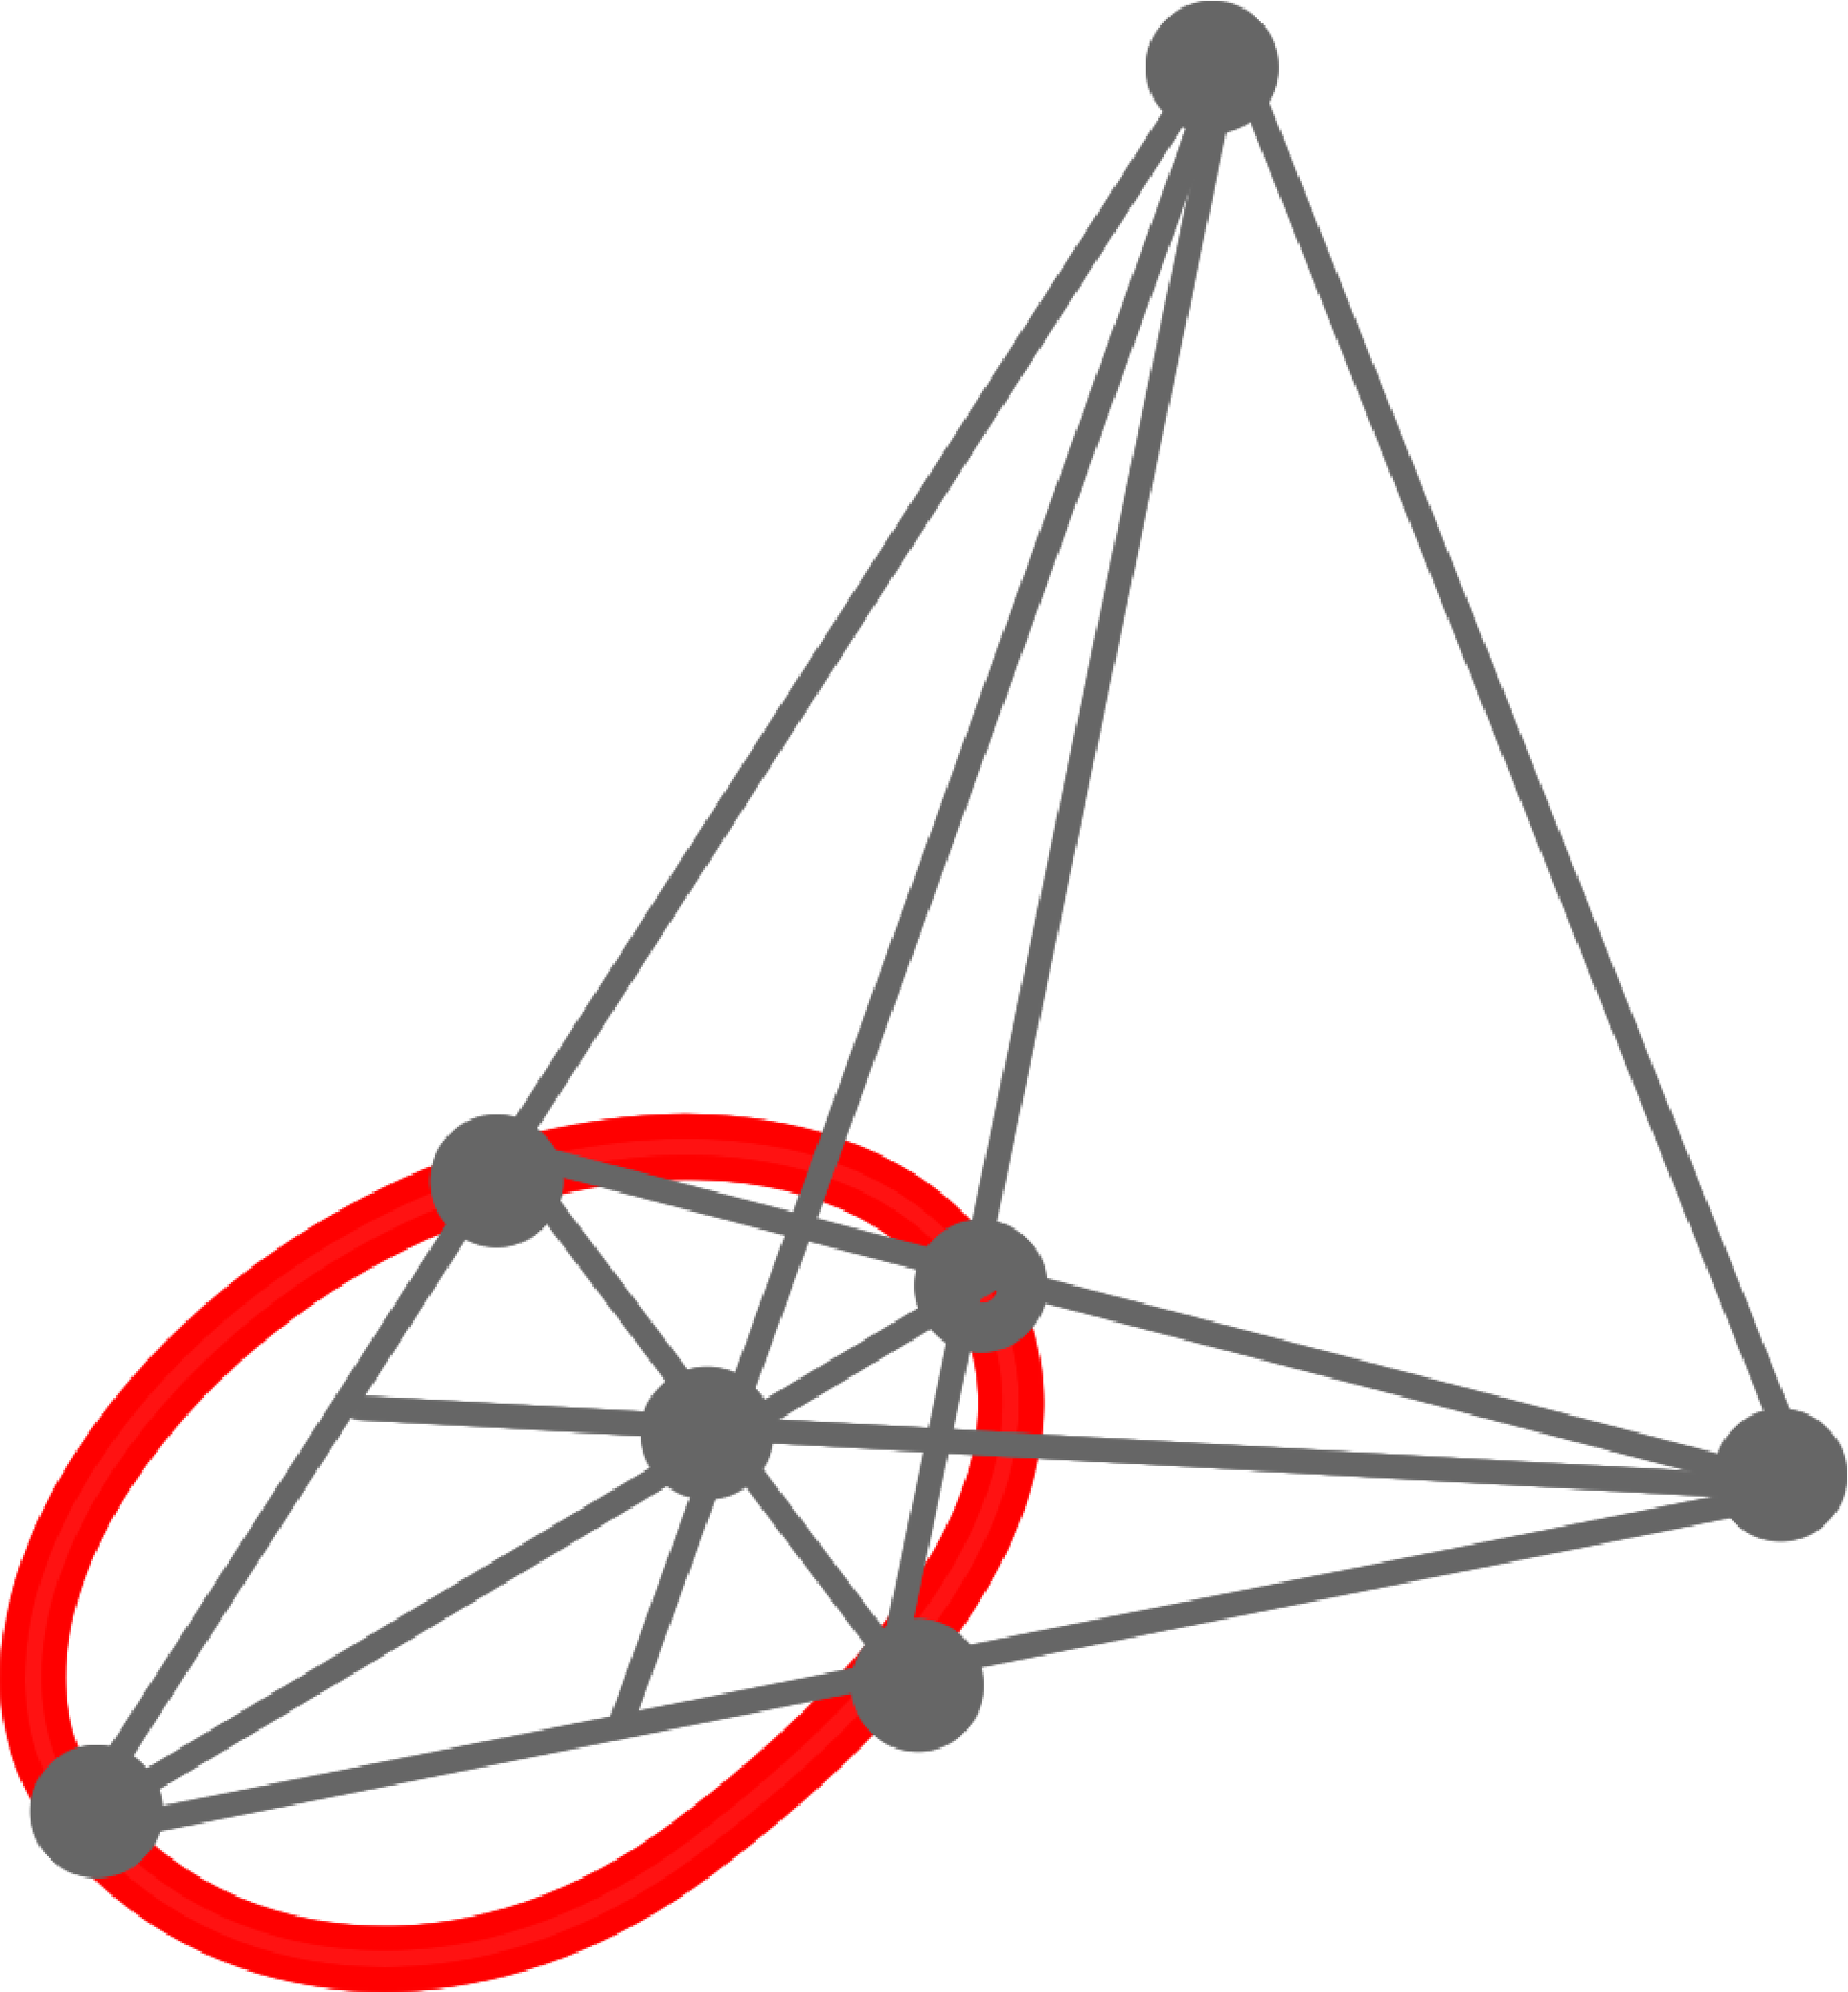
\includegraphics[width=1.4cm]{images/logo}}
 %\end{minipage}
\  \ \hfill %\begin{minipage}[t]{0.9\textwidth}
%{\color{gray}
 %\fhv{9}{Revista digital}\\
 \ %fhvb{9}{\color{azulF}Matem�tica, Educaci�n e Internet.}
  %\fntg[pag][8]{\color{grisF}
  %\href{http://www.tec-digital.itcr.ac.cr/revistamatematica/}{(http://www.tec-digital.itcr.ac.cr/revistamatematica/).}}}
%\end{minipage}          
%}%raggedright
\vspace*{3\baselineskip} % Espacio en blanco antes del final de p�gina
\endgroup}
% Fin Titulo--------------------------------------------------------





%-------------------CONTENIDO -----------------------------------------------------
\definecolor{mycolorA}{RGB}{222,122,138}  % Color de los n�meros grandes en el �ndice 
\definecolor{mycolorB}{RGB}{192,192,192} % 

% patching of \tableofcontents to use sans serif font for the tile
\patchcmd{\tableofcontents}{\contentsname}{\contentsname}{}{}
% patching of \@part to typeset the part number inside a framed box in its own line
% and to add color
\makeatletter
\patchcmd{\@part}
  {\addcontentsline{toc}{part}{\thepart\hspace{1em}#1}}
  {\addtocontents{toc}{\protect\addvspace{20pt}}
    \addcontentsline{toc}{part}{\huge{\protect\color{colordominante}%
      \setlength\fboxrule{2pt}\protect\Circle{%
        \hfil\thepart\hfil%
      }%
    }\\[2ex]\color{colordominante}\sffamily\large#1}}{}{}
\makeatother

% this is the environment used to typeset the chapter entries in the ToC
% it is a modification of the leftbar environment of the framed package
\renewenvironment{leftbar}
  {\def\FrameCommand{\hspace{6em}%
    {\color{mycolorB}\vrule width 2pt depth 6pt}\hspace{1em}}%
    \MakeFramed{\parshape 1 0cm \dimexpr\textwidth-6em\relax\FrameRestore}\vskip2pt%
  }
 {\endMakeFramed}

% using titletoc we redefine the ToC entries for parts, chapters, sections, and subsections
\titlecontents{part}
  [0em]{\centering}
  {\contentslabel}
  {}{}
\titlecontents{chapter}
  [0em]{\vspace*{2\baselineskip}}
  {\parbox{4.5em}{%
    \hfill\Huge\bfseries\color{mycolorA}\thecontentspage}%
   \vspace*{-2.3\baselineskip}\leftbar{\fhvb{12}{\chaptername~\thecontentslabel}}\\}
  {}{\endleftbar}
\titlecontents{section}
  [8.4em]
  {\sffamily\contentslabel{3em}}{}{}
  {\hspace{0.5em}\nobreak\itshape\color{mycolorA}\contentspage}
\titlecontents{subsection}
  [8.4em]
  {\sffamily\contentslabel{3em}}{}{}  
  {\hspace{0.5em}\nobreak\itshape\color{mycolorA}\contentspage}

% Fin Contenido 

%----------------------------------------------------------------------------------------
% CAPITULO Estilo simple (Donde est� la raya vertical junto al n�mero Gigante)
%----------------------------------------------------------------------------------------
 \usepackage{titlesec, blindtext, color}
 \newcommand{\hsp}{\hspace{20pt}}
 \titleformat{\chapter}[hang]{\huge\bfseries\color{colordominante}}{{
         \fontsize{5em}{5em}\selectfont\color{colordominante}
         \thechapter}\hsp\textcolor[RGB]{191,191,191}{\vrule height 4em width 2pt}\hsp}{0pt}{\huge\bfseries\color{colordominante}}
    

%----------------------------------------------------------------------------------------
%	Numeraci�n de las secciones -- en el margen
%----------------------------------------------------------------------------------------

\makeatletter
\renewcommand{\@seccntformat}[1]{\llap{\textcolor{colordominante}{\csname the#1\endcsname}\hspace{1em}}}                    
\renewcommand{\section}{\@startsection{section}{1}{\z@}
{-4ex \@plus -1ex \@minus -.4ex}
{1ex \@plus.2ex }
{\normalfont\large\sffamily\bfseries}}
\renewcommand{\subsection}{\@startsection {subsection}{2}{\z@}
{-3ex \@plus -0.1ex \@minus -.4ex}
{0.5ex \@plus.2ex }
{\normalfont\sffamily\bfseries}}
\renewcommand{\subsubsection}{\@startsection {subsubsection}{3}{\z@}
{-2ex \@plus -0.1ex \@minus -.2ex}
{0.2ex \@plus.2ex }
{\normalfont\small\sffamily\bfseries}}                        
\renewcommand\paragraph{\@startsection{paragraph}{4}{\z@}
{-2ex \@plus-.2ex \@minus .2ex}
{0.1ex}
{\normalfont\small\sffamily\bfseries}}
\makeatother
% Fin numeraci�n secciones



%---------------------------------------------------------------------------------
%  Entornos:  Ejemplo, teorema, proposici�n, lema, lista de ejercicios, 
%             caja interludio, caja simple  
%---------------------------------------------------------------------------------

%  Cajas con el paquete  tcbcolor
%  CONTADORES: ejemplo, definicion, lema, teorema, corolario, proposicion,ejercicio 
\newcounter{tcbteo}[chapter]
\renewcommand{\thetcbteo}{\thechapter.\arabic{tcbteo}}

\newcounter{tcbdefi}[chapter]
\renewcommand{\thetcbdefi}{\thechapter.\arabic{tcbdefi}}

\newcounter{tcblema}[chapter]
\renewcommand{\thetcblema}{\thechapter.\arabic{tcblema}}

\newcounter{tcbcoro}[chapter]
\renewcommand{\thetcbcoro}{\thechapter.\arabic{tcbcoro}}

\newcounter{tcbvoca}[chapter]
\renewcommand{\thetcbvoca}{\thechapter.\arabic{tcbvoca}}

%  \newcounter{tcbListaEjercicios}[chapter]
%  \renewcommand{\thetcbListaEjercicios}{\thechapter.\arabic{tcbListaEjercicios}}

\newcounter{tcbpropo}[chapter]
\renewcommand{\thetcbpropo}{\thechapter.\arabic{tcbpropo}}

\newlength{\examlen}
\tikzset{
    wnodeTeorema/.style={%
         rectangle,  top color=gray!5, bottom color=gray!5,
         inner sep=1mm,anchor=west,font=\small\bf\sffamily},
   wnodeminimo/.style={%
         rectangle,  top color=white, bottom color=white,
         text=azulF,inner sep=1mm,anchor=west,font=\small\bf\sffamily}      
}



%\begin{teorema}  o \begin{teorema}[de tal] o \begin{teorema}[][ref]
% Teorema -----------------------------------------------------
\newtcolorbox{wwteorema}[3][]{%
arc=0mm,breakable,enhanced,colback=gray!2,boxrule=0pt,top=7mm,
fontupper=\normalsize,step and label={tcbteo}{#3},
overlay unbroken = {\draw[color=colordominante,line width=0.2pt] (frame.north west)--([xshift=0pt]frame.north east);
%Caja de T�tulo: teo --
\node[wnodeTeorema](tituloteo) at ([xshift=0pt, yshift=-4mm]frame.north west)
{\textbf{\color{colordominante} Teorema \thetcbteo \;#2}};
%Borde superior --
\draw[colordominante,line width=2.5cm] ([xshift=1.25cm, yshift=0cm]frame.north west)-- +(\examlen,3pt);
},%
overlay first = {\draw[color=colordominante,line width=0.2pt] (frame.north west)--([xshift=0pt]frame.north east);
%Caja de T�tulo: teo --
\node[wnodeTeorema](tituloteo) at ([xshift=0pt, yshift=-4mm]frame.north west)
{\textbf{\color{colordominante} Teorema \thetcbteo \;#2}};
%Borde superior --
\draw[colordominante,line width=2.5cm] ([xshift=1.25cm, yshift=0cm]frame.north west)-- +(\examlen,3pt);
},%
% Mantener borde en cambio de p�gina 
overlay last = {\draw[color=colordominante,line width=0.2pt] (frame.north west)--([xshift=0pt]frame.north east);
                } 
#1}
%-
\NewDocumentEnvironment{teorema}{O{} O{} O{}}{\smallskip\begin{wwteorema}{#1}{#2}%
 #3}{\end{wwteorema}\smallskip }
% TEOREMA---------------------------------------------------------



%\begin{proposicion}  o \begin{proposicion}[de tal] o \begin{proposicion}[][ref]
% Proposici�n-----------------------------------------------------
\newtcolorbox{wwpropo}[3][]{%
arc=0mm,breakable,enhanced,colback=gray!2,boxrule=0pt,top=7mm,
fontupper=\normalsize,step and label={tcbpropo}{#3},
overlay unbroken ={\draw[color=colordominante,line width=0.2pt] (frame.north west)--([xshift=0pt]frame.north east);
%Caja de T�tulo: propo --
\node[wnodeTeorema](tituloteo) at ([xshift=0pt, yshift=-4mm]frame.north west)
{\textbf{\color{colordominante} Proposici\'on \thetcbpropo\;#2}};
%Borde superior --
\draw[colordominante,line width=2.5cm] ([xshift=1.25cm, yshift=0cm]frame.north west)-- +(\examlen,3pt);
}, %
overlay first ={\draw[color=colordominante,line width=0.2pt] (frame.north west)--([xshift=0pt]frame.north east);
%Caja de T�tulo: propo --
\node[wnodeTeorema](tituloteo) at ([xshift=0pt, yshift=-4mm]frame.north west)
{\textbf{\color{colordominante} Proposici\'on \thetcbpropo\;#2}};
%Borde superior --
\draw[colordominante,line width=2.5cm] ([xshift=1.25cm, yshift=0cm]frame.north west)-- +(\examlen,3pt);
}, %
% Mantener borde en cambio de p�gina 
overlay last ={\draw[color=colordominante,line width=0.2pt] (frame.north west)--([xshift=0pt]frame.north east);
        },
#1}
%-
\NewDocumentEnvironment{proposicion}{O{} O{} O{}}{\smallskip\begin{wwpropo}{#1}{#2}%
 #3}{\end{wwpropo}\smallskip }
% ---------------------------------------------------------



% LEMA -----------------------------------------------------------
 \newtcolorbox{wwlema}[3][]{%
arc=0mm,breakable,enhanced,colback=gray!2,boxrule=0pt,
top=1mm, left=3pt,
step and label={tcblema}{#3},
fontupper={\small\bf\sffamily {\color{azulF}Lema \thetcblema \;#2}}~\normalfont, %"Lema..."+texto del cuerpo
overlay unbroken  = {%barra vertical
\draw[color=gray,line width=3pt] ([xshift=2pt] frame.north west)--([xshift=2pt] frame.south west);                
         },%
overlay first  = {%barra vertical
\draw[color=gray,line width=3pt] ([xshift=2pt] frame.north west)--([xshift=2pt] frame.south west);                
         },%
% Mantener borde en cambio de p�gina     
overlay last ={\draw[color=gray,line width=3pt] ([xshift=2pt] frame.north west)--([xshift=2pt] frame.south west);   },    
#1}
%-
\NewDocumentEnvironment{lema}{O{} O{} O{}}{\smallskip\begin{wwlema}{#1}{#2}%
#3}{\end{wwlema}\smallskip }
%LEMA--------------------------------------------------------------


% % Corolario -------------------------------------------------------
\newtcolorbox{wwcoro}[2][]{%
arc=0mm,breakable,enhanced,colback=gray!2,boxrule=0pt,
top=1mm,left=3pt,
fontupper={\small\bf\sffamily {\color{azulF}Corolario \thetcbcoro}\;}~\normalfont, 
step and label={tcbcoro}{#2},
overlay unbroken  = {%barra vertical
\draw[color=gray,line width=3pt] ([xshift=2pt] frame.north west)--([xshift=2pt] frame.south west);                
        },%
overlay first  = {%barra vertical
\draw[color=gray,line width=3pt] ([xshift=2pt] frame.north west)--([xshift=2pt] frame.south west);                
        },%
% Mantener borde en cambio de p�gina     
overlay last ={\draw[color=gray,line width=3pt] 
                     ([xshift=2pt] frame.north west)--([xshift=2pt] frame.south west);
              }     
#1}
%-
\NewDocumentEnvironment{corolario}{O{} O{}}{\smallskip\begin{wwcoro}{#1}%
}{\end{wwcoro}\smallskip }
% Corolario------------------------------------------------------


% % Definici�n---------------------------------------------------
\newtcolorbox{wwdefinicion}[3][]{%
arc=0mm,breakable,enhanced,colback=gray!2,boxrule=0pt, %cambia el fondo de la caja
top=6mm,fontupper=\normalsize,step and label={tcbdefi}{#3},
overlay unbroken  = {
%barra vertical
\draw[color=colordominante,line width=3pt] ([xshift=2pt] frame.north west)--([xshift=2pt] frame.south west);         
%Caja de T�tulo: defi --
\node[wnodeTeorema](titulodefi) at ([xshift=4.5pt, yshift=-3mm]frame.north west)
{\textbf{\color{colordominante} Definici\'on \thetcbdefi \;#2}};
                }, %overlay
overlay first  = {
%barra vertical
\draw[color=colordominante,line width=3pt] ([xshift=2pt] frame.north west)--([xshift=2pt] frame.south west);         
%Caja de T�tulo: defi --
\node[wnodeTeorema](titulodefi) at ([xshift=4.5pt, yshift=-3mm]frame.north west)
{\textbf{Definici�n \thetcbdefi \;#2}};
                }, %overlay
% Mantener borde en cambio de p�gina
overlay last    = {%barra vertical
\draw[color=colordominante,line width=3pt] ([xshift=2pt] frame.north west)--([xshift=2pt] frame.south west);}
#1}
%-
\NewDocumentEnvironment{definicion}{O{} O{} O{}}{\smallskip\begin{wwdefinicion}{#1}{#2}%
 #3}{\end{wwdefinicion}\smallskip }
% %DEFINICION---------------------------------------------------------


% Caja para Ejemplo --------------------------------------------------
\newcounter{tcbejem}[chapter]
\renewcommand{\thetcbejem}{\thechapter.\arabic{tcbejem}}
\colorlet{colorfondoejemplo}{gray!2}
\definecolor{colorejemplo}{rgb}{.0,.0,.3}
% Ejemplo
\newtcolorbox{wwejemplo}[3][]{%
arc=0mm,
breakable,drop fuzzy shadow,
enhanced,
colback=gray!2,
boxrule=0pt,
top=8mm, %Separaci�n vertical - inicia texto
enlarge top by=\baselineskip/2+1mm,
enlarge top at break by=0mm,pad at break=2mm,
fontupper=\normalsize,
step and label={tcbejem}{#3},
overlay unbroken  = {%
%barra vertical
\draw[color=colordominante,line width=3pt] ([xshift=2pt] frame.north west)--([xshift=2pt] frame.south west);           
% Caja de imagen Ejemplo
\node[rectangle, 
         text=gray!2, 
         inner sep=1mm,anchor=west,font=\small\bf\sffamily] at ([xshift=-14.3pt,yshift=-4.1mm]frame.north west)%
{
\includegraphics{images/nodoejemplo}\raisebox{0.5cm}{}};
% Caja numeraci�n y descripci�n
\node[rectangle, 
 text=gray!2, 
 inner sep=1mm,
 anchor=west,
 font=\normalsize] at ([xshift=1.1cm,yshift=-2.9mm]frame.north west)%
 {\fhvb{10}{\;\thetcbejem \;\;\;#2}};
     }, % overlay
overlay first  = {%
%barra vertical
\draw[color=colordominante	,line width=3pt] ([xshift=2pt] frame.north west)--([xshift=2pt] frame.south west);           
% Caja de imagen Ejemplo
\node[rectangle, 
         text=gray!2, 
         inner sep=1mm,anchor=west,font=\small\bf\sffamily] at ([xshift=-14.3pt,yshift=-4.1mm]frame.north west)%
{
\includegraphics{images/nodoejemplo}\raisebox{0.5cm}{}};
% Caja numeraci�n y descripci�n
\node[rectangle, 
 text=gray!2, 
 inner sep=1mm,
 anchor=west,
 font=\normalsize] at ([xshift=1.1cm,yshift=-2.9mm]frame.north west)%
 {\fhvb{10}{\;\thetcbejem \;\;\;#2}};
     }, % overlay
%Borde cambio de p�ginas
overlay middle={\draw[color=grisamarillo,line width=3pt] ([xshift=3pt] frame.north west)--([xshift=2pt] frame.south west);},
overlay last={\draw[color=grisamarillo,line width=3pt] ([xshift=3pt] frame.north west)--([xshift=2pt] frame.south west);}
#1}
%-
\NewDocumentEnvironment{ejemplo}{O{} O{} O{}}{\smallskip\begin{wwejemplo}{#1}{#2}%
 #3}{\end{wwejemplo}\smallskip }
%EJEMPLO-----------------------------------------------------------------



% CAJA (interludio, comentario...)---------------------------------------
\definecolor{colrnodocaja}{RGB}{44,91,144}
\definecolor{colrfondocaja}{RGB}{241,241,227}

\newtcolorbox{wwcaja}[2][]{%
arc=0mm,breakable,%drop fuzzy shadow,
enhanced,colback=gray!4,
boxrule=0pt,
top=3mm, %Separaci�n vertical - inicia texto
enlarge top by=\baselineskip/2+1mm,
enlarge top at break by=0mm,pad at break=2mm,
fontupper=\normalsize,
%step and label={tcbca}{#3},
%Borde
overlay unbroken={\draw[color=gray!2,line width=0.2pt] (frame.north west)
  --([xshift=0pt]frame.north east)
  --([xshift=0pt]frame.south east)
  --([xshift=0pt]frame.south west)--(frame.north west);
% Caja de T�tulo CAJA
\node[ rectangle, %minimum width=0cm, minimum height=0.0cm,
         top color=amarilloD, bottom color=amarilloD,
         inner sep=0.5mm,anchor=west,font=\normalsize]at ([xshift=-0.5pt,  yshift=2.30mm]frame.north west){\fhvb{10}{ #2}};
         },
%Borde
overlay first={\draw[color=gray!2,line width=0.2pt] (frame.north west)
  --([xshift=0pt]frame.north east)
  --([xshift=0pt]frame.south east)
  --([xshift=0pt]frame.south west)--(frame.north west);
% Caja de T�tulo CAJA
\node[ rectangle, %minimum width=0cm, minimum height=0.0cm,
         top color=amarilloD, bottom color=amarilloD,
         inner sep=0.5mm,anchor=west,font=\normalsize]at ([xshift=-0.5pt,  yshift=2.30mm]frame.north west){\fhvb{10}{ #2}};
         },
%Borde cambio de p�gina
overlay last={\draw[color=gray!2,line width=0.2pt] (frame.north west)
  --([xshift=0pt]frame.north east)
  --([xshift=0pt]frame.south east)
  --([xshift=0pt]frame.south west)--(frame.north west);}
#1}
%-
\NewDocumentEnvironment{caja}{O{} O{}}{\smallskip\begin{wwcaja}{#1}%
 #2}{\end{wwcaja}\smallskip }
% CAJA de comentario


%CAJA simple---------------------------------------------------------------------
\newtcolorbox{wwbox}[1][]{%
arc=0mm,breakable,drop fuzzy shadow,
enhanced,colback=grisamarillo,
boxrule=0pt,
top=3mm, %Separaci�n vertical - inicia texto
enlarge top by=\baselineskip/2+1mm,
enlarge top at break by=0mm,pad at break=2mm,
fontupper=\normalsize,
%step and label={tcbca}{#3},
%Borde
overlay unbroken={\draw[color=amarilloD,line width=0.5pt] (frame.north west)
  --([xshift=0pt]frame.north east)
  --([xshift=0pt]frame.south east)
  --([xshift=0pt]frame.south west)--(frame.north west);
        },
%Borde
overlay first={\draw[color=amarilloD,line width=0.5pt] (frame.north west)
  --([xshift=0pt]frame.north east)
  --([xshift=0pt]frame.south east)
  --([xshift=0pt]frame.south west)--(frame.north west);
        },
%Borde cambio de p�gina
overlay last={\draw[color=amarilloD,line width=0.5pt] (frame.north west)
  --([xshift=0pt]frame.north east)
  --([xshift=0pt]frame.south east)
  --([xshift=0pt]frame.south west)--(frame.north west);}
#1}

 \newenvironment{scaja}[1][]{\bigskip\begin{wwbox}%
 #1}{\end{wwbox}}	
% Fin CAJA simple

%CAJA vocabulario-------------------------------------------------------
\newtcolorbox{vocabox}[3][]{%
arc=0mm,breakable,enhanced,colback=white,boxrule=0pt,
top=1mm, left=3pt,
step and label={tcbvoca}{#3},
fontupper={\small\bf\sffamily {\color{azulF}Vocabulario \thetcbvoca \;#2}}~\normalfont, %"Vocabulario..."+texto del cuerpo
overlay first  = {%barra vertical
\draw[color=white,line width=3pt] ([xshift=2pt] frame.north west)--([xshift=2pt] frame.south west);                
         },%
overlay first  = {%barra vertical
\draw[color=white,line width=3pt] ([xshift=2pt] frame.north west)--([xshift=2pt] frame.south west);                
         },%
% Mantener borde en cambio de p�gina     
overlay last ={\draw[color=white,line width=3pt] ([xshift=2pt] frame.north west)--([xshift=2pt] frame.south west);   },    
#1}
%-
\NewDocumentEnvironment{vocabulario}{O{} O{} O{}}{\smallskip\begin{vocabox}{#1}{#2}%
#3}{\end{vocabox}\smallskip }	
% Fin vocabulario

%CAJA nota-------------------------------------------------------
\newtcolorbox{notabox}[1][]{%
arc=0mm,breakable,
enhanced,colback=white,
boxrule=0pt,
top=3mm, %Separaci�n vertical - inicia texto
left=25pt,
enlarge top by=\baselineskip/2+1mm,
enlarge top at break by=0mm,pad at break=2mm,
fontupper={\begin{tikzpicture}[overlay]
\node[draw=colordominanteF,line width=1pt,circle,fill=white,font=\sffamily\bfseries,inner sep=2pt,outer sep=0pt] at (-15pt,3pt){\textcolor{colordominanteF}{N}};\end{tikzpicture}}~\normalfont,  %"NOTA..."+texto del cuerpo
%Borde y c�rculo
overlay first={
\draw[color=white,line width=0.5pt] (frame.north west)
  --([xshift=0pt]frame.north east)
  --([xshift=0pt]frame.south east)
  --([xshift=0pt]frame.south west)--(frame.north west);
        },
%Borde y c�rculo
overlay first={
\draw[color=white,line width=0.5pt] (frame.north west)
  --([xshift=0pt]frame.north east)
  --([xshift=0pt]frame.south east)
  --([xshift=0pt]frame.south west)--(frame.north west);
        },
%Borde cambio de p�gina
overlay last={\draw[color=white,line width=0.5pt] (frame.north west)
  --([xshift=0pt]frame.north east)
  --([xshift=0pt]frame.south east)
  --([xshift=0pt]frame.south west)--(frame.north west);}
#1}
%-
 \newenvironment{nota}[1][]{\bigskip\begin{notabox}%
 #1}{\end{notabox}}	
% Fin nota


%--------------------------------------------------------------------------------
% LISTAS DE EJERCICIOS
%--------------------------------------------------------------------------------
 
\usepackage{answers}
\newtheorem{exer}{}[chapter]
\newenvironment{ejer}{\begin{exer}\normalfont}{\end{exer}}
\Newassociation{solu}{Soln}{ans}

% USO del entorno personalizado---------------------------------------------------
%\begin{ejercicios} --- \end{ejercicios} para listas simples
%\begin{cejercicios} --- \end{cejercicios} para listas en cajas

\NewDocumentEnvironment{ejercicios}{O{}}{%
\bigskip\begin{minipage}{\textwidth}{\bf\verde Ejercicios}
                                     #1}{\end{minipage}\bigskip}



\colorlet{color1}{gray!5!white}       % color fondo
\definecolor{color2}{RGB}{117,184,68} % color del nodo
% Caja -- ejercicios
\newtcolorbox{wwlistaejercicios}[1][]{%
  arc=0mm,breakable,enhanced,colback=color1,boxrule=0pt,top=8mm, 
  enlarge top by=\baselineskip/2+1mm, enlarge top at break by=0mm,
  pad at break=2mm,fontupper=\normalsize,
  overlay unbroken={ % nodo rectangular  para "Ejercicios"
  \node[rectangle, minimum width=4cm, 
      top color=color2, bottom color=color2, 
      inner sep=1mm,anchor=west,font=\normalsize] 
   at ([xshift=0pt,yshift=-3mm]frame.north west)%
{\textbf{Ejercicios}};},
  overlay first={ % nodo rectangular  para "Ejercicios"
  \node[rectangle, minimum width=4cm, 
      top color=color2, bottom color=color2, 
      inner sep=1mm,anchor=west,font=\normalsize] 
   at ([xshift=0pt,yshift=-3mm]frame.north west)%
{\textbf{Ejercicios}};},
overlay last ={ } % cambio de p�gina, solo caja gris
#1}

% Nuevo entorno personalizado----------------------------------------
\NewDocumentEnvironment{cejercicios}{O{}}{%
\bigskip\begin{wwlistaejercicios}%
 #1}{\end{wwlistaejercicios}\bigskip } % 
% -------------------------------------------------------------------

% Ejercicio - Caja para ejercicio solitario
\newtcolorbox{wwejercicio}[1][]{%
arc=0mm,breakable,enhanced,colback=gray!5,boxrule=0pt,
top=1mm,left=3pt,
fontupper={\bf\sffamily {\color{miverde}Ejercicio.}\;}~\normalfont, 
overlay unbroken  = {%barra vertical
\draw[color=gray,line width=3pt] ([xshift=2pt] frame.north west)--([xshift=2pt] frame.south west);               
        },%
overlay first  = {%barra vertical
\draw[color=gray,line width=3pt] ([xshift=2pt] frame.north west)--([xshift=2pt] frame.south west);               
        },%
% Mantener borde en cambio de p�gina     
overlay last ={\draw[color=gray,line width=3pt] 
                     ([xshift=2pt] frame.north west)--([xshift=2pt] frame.south west);
              }     
#1}


% Entorno con Caja para ejercicios-----------------------------------------
%\begin{cajaejercicios}  o \begin{cajaejercicios}[de tal] 
%                        o \begin{cajaejercicios}[][ref]
% Entorno personalizado---------------------------------------------------
\definecolor{colorejercicios}{RGB}{99,42,134}
\newcounter{tcbejer}[chapter]
\renewcommand{\thetcbejer}{\thechapter.\arabic{tcbejer}}

\newtcolorbox{wwejercicios}[3][]{%
arc=0mm,breakable,%drop fuzzy shadow,
enhanced,colback=gray!5,boxrule=0pt,top=7mm,
fontupper=\normalsize,step and label={tcbejer}{#3},
overlay unbroken = {
%Borde grueso superior
\draw[color=colorejercicios,line width=3pt] (frame.north west)--([xshift=0pt]frame.north east);
%Caja de T�tulo: Ejer --
\node[rounded corners=3pt,  draw=colorejercicios, top color=white, bottom color=white, thick,inner sep=1mm,anchor=west, font=\small\bf\sffamily](tituloejer) at ([xshift=5mm, yshift=0mm]frame.north west)
{\textbf{\color{miverde}  Ejercicios \thetcbejer \;#2}};
%borde l�nea inferior
 \draw[color=colorejercicios,line width=0.2pt] (frame.south west)--([xshift=0pt]frame.south east); 
},%overlay
overlay first = {
%Borde grueso superior
\draw[color=colorejercicios,line width=3pt] (frame.north west)--([xshift=0pt]frame.north east);
%Caja de T�tulo: Ejer --
\node[rounded corners=3pt,  draw=colorejercicios, top color=white, bottom color=white, thick,inner sep=1mm,anchor=west, font=\small\bf\sffamily](tituloejer) at ([xshift=5mm, yshift=0mm]frame.north west)
{\textbf{\color{miverde}  Ejercicios \thetcbejer \;#2}};
%borde l�nea inferior
 \draw[color=colorejercicios,line width=0.2pt] (frame.south west)--([xshift=0pt]frame.south east); 
},%overlay
% % Mantener borde en cambio de p�gina 
% overlay middle = {\draw[color=colordominante,line width=0.2pt] (frame.north west)--([xshift=0pt]frame.north east);
%                 } 
overlay middle ={},
overlay last = { %borde l�nea inferior
 \draw[color=colorejercicios,line width=0.2pt] (frame.south west)--([xshift=0pt]frame.south east); 
                } 
#1}
%-
\NewDocumentEnvironment{cajaejercicios}{O{} O{} O{}}{\smallskip\begin{wwejercicios}{#1}{#2}%
 #3}{\end{wwejercicios}\smallskip }
% ejercicios---------------------------------------------------------


% Comandos para paquete answers
% pregunta-soluci�n
\newcommand{\exersol}[2]{
\begin{ejer} 
#1\scantokens{\begin{solu}#2\end{solu}}
\end{ejer}}
% listas \item pregunta-soluci�n
\newcommand{\itemps}[2]{\item #1\scantokens{\begin{solu}#2\end{solu}}}

\newcommand{\bex}{\scantokens{\begin{solu} \end{solu}}\begin{enumerate}[label=\alph*.)]}
\newcommand{\eex}{\end{enumerate}}
%\begin{sol} \end{sol}


%-
\NewDocumentEnvironment{ejercicio}{O{} O{}}{\smallskip\begin{wwejercicio}{#1}%
}{\end{wwejercicio}\smallskip }
% Ejercicio------------------------------------------------------



% -- Soluciones al final del documento----------------------------
\def\soluciones{
\expandafter\ifx\csname Closesolutionfile\endcsname \relax\else
\Closesolutionfile{ans}\fi
}

\def\solucionesCap#1{\section*{Soluciones del Cap\'{\i}tulo #1}\input{ans#1}}
% Fin Listas de Ejercicios-------------------------------------------


% Fin mis entornos---------------------------------------------------------------


%---------------------------------------------------------------------------------
%  C�digo de programas (LaTeX en ese caso)
%---------------------------------------------------------------------------------
% Listings
\usepackage{listings}% uso: \lstinline|section|
\lstset{ %
	      language={[LaTeX]TeX}, % lenguaje
	      basicstyle=\bfseries\ttfamily,
	      keywordstyle=\color{blue},
	      commentstyle=\color{brown},	   
	      backgroundcolor=\color{grisamarillo},
	      showstringspaces=false,
	      flexiblecolumns=true,
	      stringstyle=\ttfamily\color{blue},
	      extendedchars=true,
emph={rm,bf,it,sf,sl,sc,tt,gtrdot,lesseqqgtr,Supset,mathbb,gtrless,doteqdot,sqsubset,mathbb,eqslantless,risingdotseq,sqsupset,mathbb,lesssim,fallingdotseq,succcurlyeq,therefore,lessapprox,circeq,preccurlyeq,because,approxeq,triangleq,curlyeqprec,leqq,lessdot,thicksim,curlyeqsucc,geqq,gtreqless,thickapox,precsim,leqslant,gtreqqless,backsim,succsim,geqslant,lll,backsimeq,precapprox,eqslantgtr,ggg,subseteqq,succapprox,gtrsim,lessgtr,supseteqq,vartriangleright,gtrapprox,lesseqgtr,Subset,trianglerighteq,maxint,for,to,do
},
    emphstyle={\color{blue}\textbf}
	      }
\newcommand{\wlatex}{\lstinline}


%---------------------------------------------------------------------------------
%  Listas con Tikz 
%---------------------------------------------------------------------------------
% Puntos Tikz y  Enumerate con  Tikz 
  \newcommand{\tpto}{\tikz \shadedraw [shading=ball] (0,0) circle (.1cm);}
  \newcommand{\ttpto}[1]{\begin{tikzpicture}
  	\node[scale=.5, circle, shade, ball color=blue]  {\color{white}\Large\textbf#1};
  \end{tikzpicture}}
  \newcommand{\ttptov}{\begin{tikzpicture}
  	\node[scale=.5, circle, shade, ball color=green]  {\color{white}\Large\textbf.};
  \end{tikzpicture}}
  \newcommand{\ttptor}{\begin{tikzpicture}
  	\node[scale=.5, circle, shade, ball color=red]  {\color{white}\Large\textbf.};
  \end{tikzpicture}}
  \newcommand{\ptoazul}[1]{\begin{tikzpicture}
  	\node[scale=.5, circle, shade, ball color=blue]  {\color{white}\Large\textbf#1};
  \end{tikzpicture}}
 \newcommand{\ptomb}{\ptoazul$\;$}
 \newcommand{\itempto}{\item[\tpto]}
 \newcommand{\pto}{\tpto}
 \newcommand{\ptom}{\tpto$\;$}
 \newcommand{\ptomv}{\ttptov$\;$}
 \newcommand{\ptomr}{\ttptor$\;$}

 % Listas -- con puntos

 %\usepackage{enumerate}
 \newcommand{\witem}[1]{\item[{\bf #1)}]}
 
 \newcommand*{\itembolasgrises}[1]{%
 \footnotesize\protect\tikz[baseline=-3pt]%
 \protect\node[fill=gray!50,shape=circle,draw,inner sep=1.2pt,line width=0.2mm](n1){#1};}
 \newcommand*{\itembolasazules}[1]{%
 \footnotesize\protect\tikz[baseline=-3pt]%
 \protect\node[scale=.5, circle, shade, ball color=blue]  {\color{white}\Large\bf#1};}
 \newcommand*{\itembolasverdes}[1]{%
 \footnotesize\protect\tikz[baseline=-3pt]%
 \protect\node[scale=.5, circle, shade, ball color=green]  {\color{white}\Large\bf#1};}
 \newcommand*{\itembolasrojas}[1]{%
  \footnotesize\protect\tikz[baseline=-3pt]%
  \protect\node[scale=.5, circle, shade, ball color=red]  {\color{white}\Large\bf#1};}
  
%Comando para listas con bolas	
\newcommand{\beaz}{\begin{enumerate}[label=\itembolasazules{\arabic*}]}
\newcommand{\eeaz}{\end{enumerate}}
% Fin de cosas adicionales -


%-----------------------------------------------------------------------------
% TABLAS CON Tikz
%----------------------------------------------------------------------------- 
\usepackage{array}
\usetikzlibrary{calc,fit,shadows,arrows,positioning}
\pgfdeclarelayer{background}
\pgfdeclarelayer{foreground}
\pgfsetlayers{background,main,foreground}
%--
%------------------------------------------------------------------------------
% Data Table
%------------------------------------------------------------------------------
\newsavebox{\dataTableContent} % Box
\newenvironment{dataTable}[1] % \new environment
{%
\begin{lrbox}{\dataTableContent}%
\begin{tabular}{#1}}%
%
{%
\end{tabular}
\end{lrbox}
\begin{tikzpicture}
\node [inner xsep=0pt] (tbl){\usebox{\dataTableContent}};
\begin{pgfonlayer}{background}
% table
\draw[rounded corners=1pt,top color=gray!1,bottom color=gray!30,draw=black]
(tbl.north east) rectangle (tbl.south west);
% top line
\draw[rounded corners=1pt,top color=gray!10!black,bottom color=gray!50!black,draw=black]%
($(tbl.north west)$) rectangle ($(tbl.north east)-(0,1.5\baselineskip)$);
% bottom rule
\draw[rounded corners=0.25pt,fill=gray,draw=black]%
(tbl.south west) rectangle ($(tbl.south east)+(0,0.05)$);
\end{pgfonlayer}
\end{tikzpicture}}
% --
 
 
 
%----------------------------------------------------------------------------- 
%- Modoficaci�n de chapter para que abra y cierre archivos ans----------------
%-----------------------------------------------------------------------------

%-------------------------------------------------------------------------------
%- Modoficaci�n de chapter para que abra y cierre archivos ans del paquete answers                                   
\newcount\ansj % contador de listas ans i
\ansj=\thechapter
%           % -- Infiltrar \chapter --------------------------------------------
\makeatletter
\let\stdchapter\chapter % \stdchapter guarda la def original de \chapter
\renewcommand*\chapter{ % -- Infiltrar: abrir y cerrar archivos ans j---
\expandafter\ifx\csname Closesolutionfile\endcsname \relax\else
\Closesolutionfile{ans}\fi
\expandafter\ifx\csname Opensolutionfile\endcsname \relax\else
\Opensolutionfile{ans}[ans\number\ansj]\advance\ansj by 1\fi
                        %------------------------------------------------------
                        % Volver a la def original de \chapter
\@ifstar{\starchapter}{\@dblarg\nostarchapter}}
\newcommand*\starchapter[1]{\stdchapter*{#1}}
\def\nostarchapter[#1]#2{\stdchapter[{#1}]{#2}}
\makeatother
 % -- -------------------------------------------------------------------------
 

 
 
%----------------------------------------------------------------------------------------
% Comandos del libro
%----------------------------------------------------------------------------------------

%----------------------------------------------------------------------------------------








% = Paquetes y c�digo de dise�o
%----------------------------------------------------------------------

\geometry{bindingoffset=2cm}
\geometry{textwidth = 125.652mm,textheight = 170mm}

%-----------------------------------------------------------------------
% COMANDOS PERSONALES
%-----------------------------------------------------------------------
\newcommand{\R}{\mathbb{R}}
\newcommand{\Z}{\mathbb{Z}}
\newcommand{\Q}{\mathbb{Q}}
\newcommand{\N}{\mathbb{N}}
\newcommand{\I}{\mathbb{I}}
\newcommand{\raya}{\rule{2cm}{0.01cm}\\}
\newcommand{\ds}{\displaystyle}
\newcommand{\sen}{\mathop{\rm sen}\nolimits}
\newcommand{\senh}{\mathop{\rm senh}\nolimits}
\newcommand{\arcsen}{\mathop{\rm arcsen}\nolimits}
\newcommand{\arcsec}{\mathop{\rm arcsec}\nolimits}
\newcommand{\bc}{\begin{center}}
\newcommand{\ec}{\end{center}}
\newcommand{\be}{\begin{enumerate}}
\newcommand{\ee}{\end{enumerate}}
\newcommand{\lenginf}{{\mathscr{L}_{\scriptscriptstyle \kappa \, \scriptscriptstyle \lambda}}}
\newcommand{\leninf}[2]{\mathscr{L}_{\scriptscriptstyle #1 \, \scriptscriptstyle #2}}
\newcommand{\pot}{\mathscr{P}}
\newcommand{\indpeq}{\scriptscriptstyle}
\newcommand{\sii}{si y solo si }
\newcommand{\no}{\neg}
\newcommand{\oinf}{\bigvee}
\newcommand{\yinf}{\bigwedge}
\newcommand{\ent}{\rightarrow}
\newcommand{\syss}{\leftrightarrow}
\newcommand{\subcuant}[2]{\underset{\scriptscriptstyle #1 < \scriptscriptstyle #2}}
\newcommand{\term}[2]{\textbf{\textit{Exp}}_{#1 \, #2}}
\newcommand{\form}[2]{\textit{\textbf{Form}}_{#1 \, #2}}
\newcommand{\atom}[2]{\textit{\textbf{Atom}}_{#1 \, #2}}
\newcommand{\enu}[2]{{\large ${\mathscr{L}_{\scriptscriptstyle #1 \, \scriptscriptstyle #2}^{\scriptscriptstyle 0}}$}}
\newcommand{\arbol}{\textit{\'arbol}}


%----------- Comandos del otro documento ------------------
\newcommand\ddfrac[2]{\frac{\displaystyle #1}{\displaystyle #2}}
\DeclareMathOperator{\atantwo}{atan2}
\renewcommand{\tablename}{Tabla}



%----------------------------------------------------------





\begin{document}

\frontmatter
	
%-----------------------------------------------------------------------------------
%                                  PORTADA
%-----------------------------------------------------------------------------------

%\parindent=0mm    % Sangr�a
%\pagestyle{empty}
%\titulo{% T�tulo 
%           \fntb[ppl][14]{T�TULO, YO}
%        }{% Autor
%          \fntb[ppl][12]{DocDoc}
6%       }{% Adicional
%       \fntb[ppl][10]{Agosto, 2017.}}

%-----------------------------------------------------------------------------------  
  
  
% %---------------------------------------------------------------------------------
% %	                          Tabla de contenidos
% %---------------------------------------------------------------------------------
 
\tableofcontents
\thispagestyle{empty}

%-----------------------------------------------------------------------------------


% %---------------------------------------------------------------------------------
% %                           Prefacio o Pr�logo  
% %---------------------------------------------------------------------------------
%\begin{prologo}
% Bueno, aqu� viene el pr�logo de este libro...\\\\
%\textit{M\'exico, D.F., 2017.} \hfill{\sc Nombre}
%\end{prologo}
\mainmatter
%-----------------------------------------------------------------------------------


%-----------------------------------------------------------------------------------
%                                 Inicio
%-----------------------------------------------------------------------------------
\cleardoublepage
\pagestyle{fancy}                      % Habilitar encabezados
\pagenumbering{arabic}                 % Numeraci�n arabiga
\ansj=1                                % Cap 1 inicializa listas 
%-----------------------------------------------------------------------




%------------------------------------------------------------------------------------
%	Cap�tulo 1
%------------------------------------------------------------------------------------
\chapter{Introducción y Generalidades}

\section{Introducción}
Tipos de arquitecturas de los robots móviles.

\section{Modelos Tradicionales}
Características

Se tiene representación del medio ambiente

\begin{figure}[h!]
	\centering
	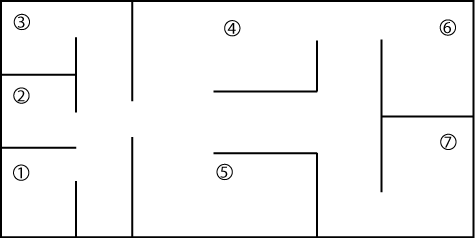
\includegraphics[width=0.5\textwidth]{images/img1.png}
	\captionof{figure}{(Objeto mesa (cuarto 1 $x_{_1}y_{_1},x_{_2}y_{_2},...,x_{_n}y_{_n}$))}
	\label{figura1}
\end{figure}

\paragraph{}
Se planean las acciones y los movimientos del robot.

\begin{wrapfigure}{l}{45 mm}
  \begin{center}
    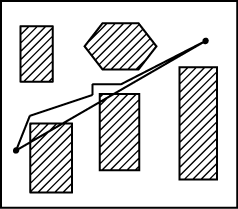
\includegraphics[width = 2 cm]{images/img2.png}
  \end{center}
    
\end{wrapfigure}

El robot debe llegar de 1 a 6. Dado que el robot conoce el mapa del lugar puede trazar un árbol y encontrar lo mejor ruta (rama de menor peso).

Sin embargo, desconoce los objetos que obstruyen su camino; por lo que no debe descartar las otras ramas.

\begin{wrapfigure}{l}{45 mm}
  \begin{center}
    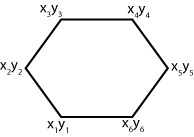
\includegraphics[width = 3 cm]{images/img3.png}
  \end{center}
    
\end{wrapfigure}


Si se conocen objetos obstáculo, se aproximan a polígonos y se almacenan sus vértices. Si uno intersecta el camino de línea recta entre origen y destino, el robot se desplaza a la esquina más cercana y bordea el obstáculo.

\begin{figure}[h!]
	\centering
	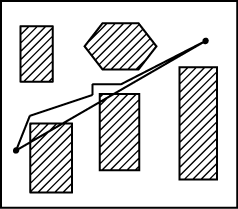
\includegraphics[width=0.35\textwidth]{images/img2.png}
\end{figure}

Se tiene una organización serial, si un modulo falla... 
Se tiene un grupo de sensores para detectar el medio ambiente
\\
\\

\begin{figure}[h!]
	\centering
	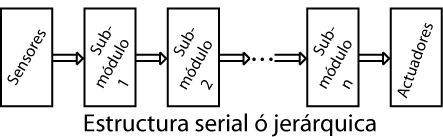
\includegraphics[width=0.55\textwidth]{images/img4.png}
	\label{figura4}
\end{figure}

Este tipo de sistemas no es adecuado para entornos dinámicos y para robots que presentan errores en el movimiento y sensado.



\section{Modelos Reactivos}


Características:

\begin{itemize}
	\item[\textbullet] Basado en el comportamiento de los insectos
	\item[\textbullet] No es necesaria una representación del medio ambiente
	\item[\textbullet] No utiliza planeación de acciones ni de movimiento
	\item[\textbullet] Es adecuado para entornos dinámicos y con errores en el sensado
	\item[\textbullet] Esta basado en comportamientos funcionando en paralelo.
\end{itemize}

\newpage

\begin{figure}[h!]
	\centering
	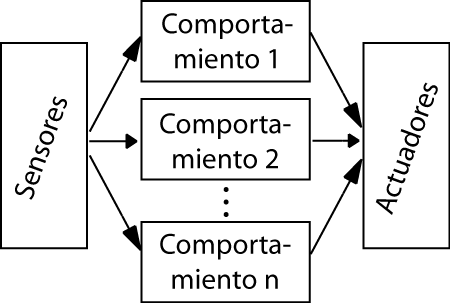
\includegraphics[width=0.5\textwidth]{images/img5.png}
	\label{figura6}
\end{figure}

La salida de cada comportamiento debe ser instantánea a partir del momento que hay una entrada.
Los comportamientos son independientes entre si.
Por ejemplo si se tienen un grupo de robots en un campo con discos con la siguiente programación:

\begin{enumerate}
	\item Moverse aleatoriamente hasta 2 o 3 
	\item Si se encuentra disco y no se porta disco, recoger el disco $\rightarrow1$
	\item Si se encuentra disco y se porta disco soltar el disco $\rightarrow1$
\end{enumerate}



\section{Modelos Híbridos}

Se combinan las arquitecturas tradicionales y reactivas para suplir las deficiencias de cada una de ellos.

\begin{figure}[h!]
	\centering
	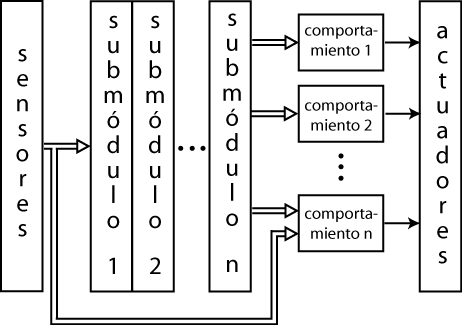
\includegraphics[width=0.5\textwidth]{images/img6.png}
	\label{figura6}
\end{figure}



\section{Comportamientos Reactivos}

Se manejan mediante diagramas estimulo- respuesta o ER

\begin{figure}[h!]
	\centering
	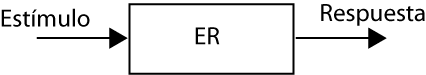
\includegraphics[width=0.4\textwidth]{images/img7.png}
	\label{figura7}
\end{figure}

\paragraph{}
O bien

\begin{figure}[h!]
	\centering
	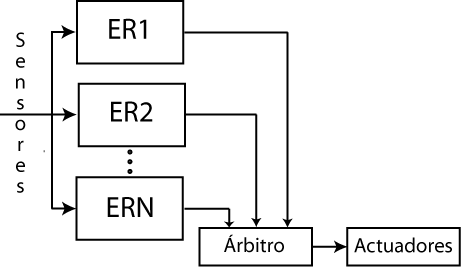
\includegraphics[width=0.5\textwidth]{images/img8.png}
	\label{figura8}
\end{figure}

\paragraph{}
O bien

\begin{figure}[h!]
	\centering
	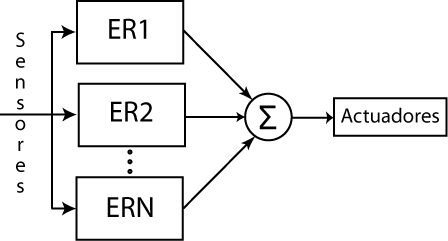
\includegraphics[width=0.5\textwidth]{images/img9.png}
	\label{figura9}
\end{figure}


\paragraph{}

Inteligencia espontánea: los robots hacen algo que no sabrán que estaban haciendo.
En un robot que tiene varios comportamientos coordinados por un agente, todos los comportamientos deben ofrecer una salida por ciclo de reloj, es decir, un comportamiento debe dar salida inmediata.

\begin{figure}[h!]
	\centering
	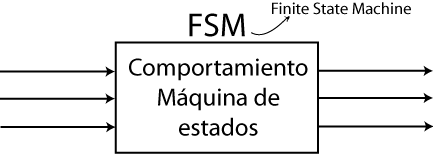
\includegraphics[width=0.5\textwidth]{images/img10.png}
	\label{figura10}
\end{figure}

\paragraph{}
Ronald Brooks propone

\begin{figure}[h!]
	\centering
	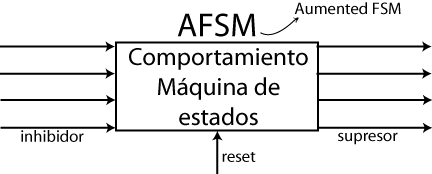
\includegraphics[width=0.5\textwidth]{images/img11.png}
	\label{figura11}
\end{figure}

\paragraph{}
Tenemos entonces:

\begin{figure}[h!]
	\centering
	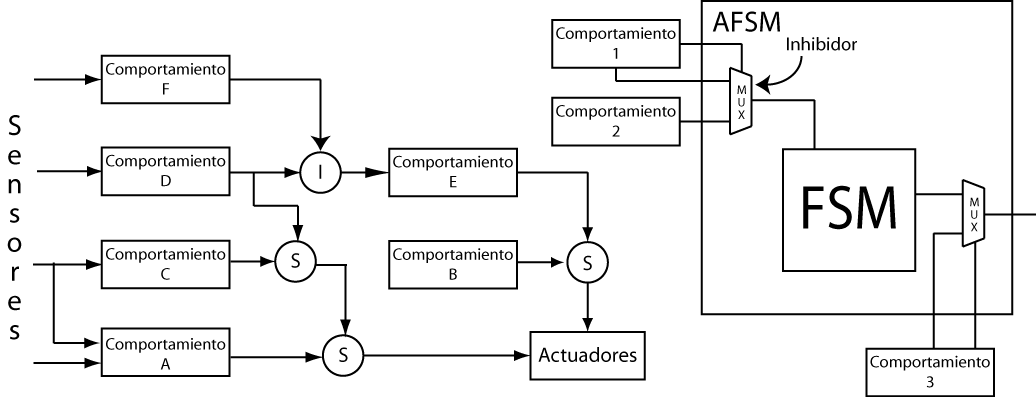
\includegraphics[width=1\textwidth]{images/img12.png}
	\label{figura12}
\end{figure}


\section{Campos Potenciales}

El destino se determina por un capo potencial de atracción y los obstáculos como campos potenciales de repulsión.

\begin{figure}[h!]
	\centering
	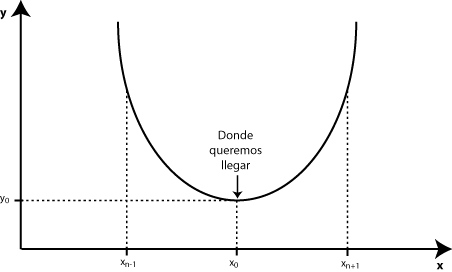
\includegraphics[width=0.5\textwidth]{images/img13.png}
	\label{figura13}
\end{figure}

% NOTA creo que aquí no es x - 1 sino n - 1

$$x_{n} = f(x_{n - 1}) = x_{x - 1} \, \delta \; \dfrac{dy}{dy}$$

Por ejemplo para una parábola \hspace{1cm} $y = y_{0} + (x - x_{0})^2$ 

$$\;\dfrac{dy}{dx} = 2(x - x_{0})$$ 
\hspace{2cm} \textit{si} $\delta = \dfrac{1}{2}$ $\Rightarrow$ $x_{n - 1} = -\dfrac{1}{2} (2(x_{n - 1} - x_{0})) = x_{0}$, \textit{llegamos en un paso}.

\paragraph{}
Esta técnica se conoce como: descendiendo por la pendiente más pronunciada o steppest descent.

\hspace{2cm}$\overline{q}_{n} = [x_n,y_n]$ \hspace{0.5cm} \textit{la posición del robot} \hspace{0.5cm}  $\overline{q}_{n} = \overline{q}_{n - 1} - \delta \overline{f} \left( \overline{q}_{n - 1} \right)$ \hfill \break
\hspace{1cm} \textit{donde} $\overline{f} \left( \overline{q}_{n - 1}\right)$ \textit{es un vector fuerzas unitario en la dirección del gradiente} $\overline{f}(\overline{q}) = \dfrac{\overline{F(\overline{q})}}{\left| \overline{F}(\overline{q})\right|}$ 
\hfill \break
\textit{donde} $\overline{F}(\overline{q}) = \nabla U(\overline{q}) = \left( \dfrac{\partial u}{\partial x} \,\hat{i} + \dfrac{\partial u}{\partial x}\, \hat{j} \right)$ 

El gradiente del campo potencial \hspace{1cm} \textit{donde}  $u(\overline{q}) = U_{\mbox{\textit{atracción}}}(\overline{q}) + U_{\mbox{\textit{repulsión}}}(\overline{q})$

Los campos potenciales atractivos y repulsivos y  $\overline{F}(\overline{q}) = \overline{F}_{atr}(\overline{q}) + \overline{F}_{rep}(\overline{q})$ las fuerzas de atracción y repulsión

\begin{figure}[h!]
	\centering
	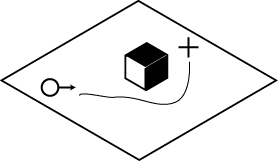
\includegraphics[width=0.5\textwidth]{images/img14.png}
	\label{figura14}
\end{figure}



\section{Campos Potenciales Atractivos}

\begin{center}


$\overline{q} = (x,y)$ \textit{Es la posición del robot}

$\overline{q}_{dest} $ \textit{Posición del punto al que queremos llegar}

$\overline{F}_{atr}(\overline{q}) = \epsilon_{1} (\overline{q} - \overline{q}_{dest})$ \textit{siempre que} $\left| \overline{q} - \overline{q}_{dest} \right| \leq d_{i}$ \textit{para} $\left| \overline{q} - \overline{q}_{dest} \right| > d_{i}$, $U_{atr}(\overline{q}) = \epsilon_{2} \left| \overline{q} - \overline{q}_{dest} \right|$ \textit{o bien,} 
\end{center}

$$U_{atr}(x,y) = \epsilon_{2} \left( (x - x_{0})^2 + (y - y_{0})^2 \right)^\frac{1}{2}$$
$$\dfrac{\partial U_{atr}(x,y)}{\partial x} = \dfrac{\epsilon_{2}2(x - x_{0})}{2\sqrt{(x - x_{d})^2 + (y - y_{d})^2}}$$
$$\dfrac{\partial U_{atr}(x,y)}{\partial y} = \dfrac{\epsilon_{2}(y - y_{0})}{\sqrt{(x - x_{d})^2 + (y - y_{d})^2}}$$
$$\Rightarrow \nabla U_{atr(x,y)} = \dfrac{\epsilon_{2}\left( (x - x_{0}) + (y - y_{d})\right) }{\sqrt{(x - x_{d})^2 + (y - y_{d})^2}} = \dfrac{\epsilon_{2}(\overline{q} - \overline{q}_d)}{\left| \overline{q} - \overline{q}_{d} \right|} = F_{atr}(\overline{q})$$


\section{Campos Potenciales Repulsivos}

\begin{figure}[h!]
	\centering
	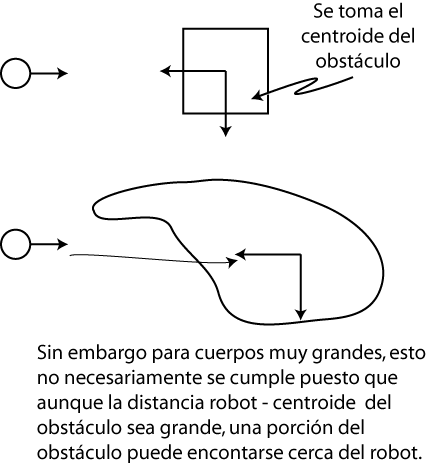
\includegraphics[width=0.7\textwidth]{images/img15.png}
	\label{figura15}
\end{figure}
\newpage

$$\left| \overline{q} - \overline{q}_{obs}\right| \leq d_{0}$$

$$U_{rep}(\overline{q}) = \dfrac{1}{2} \eta \left( \dfrac{1}{\left| \overline{q} - \overline{q}_{obs}\right|}  
- \dfrac{1}{d_{0}} \right)^2$$

$$U_{rep}(x,y) = \dfrac{1}{2} \eta \left( \dfrac{1}{\sqrt{(x - x_{obs})^2 + (y - y_{obs})^2}}  
- \dfrac{1}{d_{0}} \right)^2$$

$$\dfrac{\partial U_{rep}(x,y)}{\partial x} = \eta \left( \dfrac{1}{d_{0}}  
-  \dfrac{1}{\sqrt{(x - x_{obs})^2 + (y - y_{obs})^2}} \right)^2 \left( \dfrac{x - x_{obs}}{\left( (x - x_{obs})^2 + (y - y_{obs})^2 \right)^{\frac{3}{2}}} \right)$$

$$\dfrac{\partial U_{rep}(x,y)}{\partial y} = \eta \left( \dfrac{1}{d_{0}}  
-  \dfrac{1}{\sqrt{(x - x_{obs})^2 + (y - y_{obs})^2}} \right)^2 \left( \dfrac{y - y_{obs}}{\left( (x - x_{obs})^2 + (y - y_{obs})^2 \right)^{\frac{3}{2}}} \right)$$

$$\nabla U_{rep}(\overline{q}) = -\eta \left( \dfrac{1}{\left| \overline{q} - \overline{q}_{obs}\right|} - \dfrac{1}{d_{0}} \right)  \left( \dfrac{1}{\left| \overline{q} - \overline{q}_{obs}\right|^2}\right)  \left( \dfrac{\overline{q} - \overline{q}_{obs}}{\left| \overline{q} - \overline{q}_{obs}\right|}\right) = \overline{F}_{rep}(\overline{q})$$

\paragraph{}
Fuerza de repulsión del obstáculo $k$

\begin{center}
$\overline{F}_{rep}(\overline{q}) = 0$ \textit{ si } $\left| \overline{q} - \overline{q}_{obs}\right| > 0$
\end{center}

$$\overline{F}(\overline{q}) = \overline{F}_{atr}(\overline{q}) + \displaystyle \sum_{i = 1}^{n} \, \overline{F}_{rep}(\overline{q})$$

Luego

$$f(\overline{q}) = \dfrac{\overline{F}(\overline{q})}{\left|  \overline{F}(\overline{q}) \right| }$$


$$\overline{q}_{i + 1} = \overline{q}_{i} - \delta_{i} \overline{f}(q_{i})$$

Ejemplo:

\begin{figure}[h!]
	\centering
	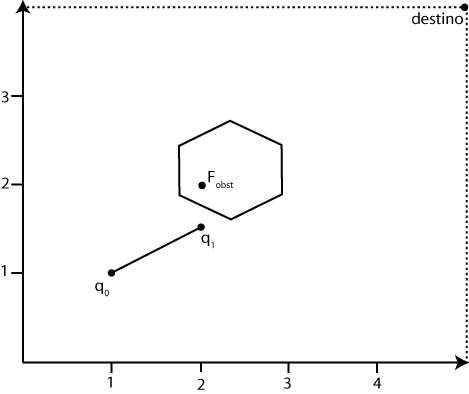
\includegraphics[width=0.7\textwidth]{images/img16.png}
	\label{figura16}
\end{figure}

$$\overline{q}_{0} = (1,1),\, \overline{q}_{obs} = (2,2),\, \overline{q}_{dest} = (5,4),\, d_{0} = 5,\, \epsilon_{1} = 5, \,\, \eta = 2,\, \delta_{0} = 1,\, \delta_{1} = 10$$

$$\overline{F}_{atr}(\overline{q}_{0}) = \overline{F}_{atr}(1,1) = \epsilon_{1}(\overline{q}_{0} - \overline{q}_{dest}) = 1((1,1) - (5,4)) = (-4,-3)$$

$$\overline{F}_{rep}(\overline{q}_{0}) = \left( -2\left( \dfrac{1}{\sqrt{2}} - \dfrac{1}{5} \right) \left( \dfrac{1}{2} \right)  \left( \dfrac{(-1,-1)}{\sqrt{2}} \right) \right) = (0\ldotp3585,0\ldotp3585)$$

$$\overline{F}(\overline{q}) = (-4,-3) + (0\ldotp3585,0\ldotp3585) = (-3\ldotp64,-2\ldotp64)$$

$$f(\overline{q}) = \dfrac{(-3\ldotp64,-2\ldotp64)}{|4\ldotp4985|} = (-0\ldotp8091,-0\ldotp5868)$$
$$ \Rightarrow q_{1} = q_{0} - \delta_{0}\,\overline{f}(\overline{q}_{0}) = (1,1) + (-0\ldotp8091,-0\ldotp5868)$$
$$\Rightarrow q_{1} = (1\ldotp8091,1\ldotp5868)$$

Encontrar los siguientes tres puntos de posicionamiento del robot. Obtenga $q_{2}$, $q_{3}$ y $q_{4}$.


\section{Campos Potenciales Usando Sensores de Proximidad}

%imagen

En el ángulo de determina hacia donde mira el robot respecto a su posición alfa es el ángulo del sensor respecto a la orientación del robot. 

D es la distancia reportada por el sensor al obstáculo. 

$$x_{obs} = d\cos (\theta + \alpha)$$
$$y_{obs} = d\sen (\theta + \alpha)$$
$$\overline{q} - \overline{q}_{obs} = (0,0) - (x_{obs}, y_{obs}) = (-x_{obs}, -y_{obs})$$

%imagen

Cuando se conoce la posición de los objetos se puede almacenar en una matriz el campo de repulsión. Esto requiere de un procesador más potente.

%imagen

Dados $(x_{i - 1}, y_{i - 1})$ para llegar al punto $(x_{i}, y_{i})$ se desea saber el ángulo que el robot debe girar para llegar a su destino, o bien el desplazamiento.

$$x_{i} = \overline{OA} = x_{i - 1} + r\cos (\theta_{i - 1} = \theta_{i})$$
$$y_{i} = \overline{AP} = y_{i - 1} + r\sen (\theta_{i - 1} = \theta_{i})$$
$$x_{i} = x_{i}^{\,\prime} \cos (\theta_{i - 1}) - y_{i}^{\,\prime} \sen (\theta_{i - 1}) + x_{i - 1}$$

$$y_{i} = x_{i}^{\,\prime} \sen (\theta_{i - 1}) - y_{i}^{\,\prime} \cos (\theta_{i - 1}) + y_{i - 1}$$

Esto para un sistema omnidireccional. En forma matricial:

$$
\begin{bmatrix}
x_{i} \\
y_{i} \\
\theta_{i}
\end{bmatrix} = \begin{bmatrix}
\cos (\theta_{i - 1}) & \sen (\theta_{i - 1}) & 0 \\
\sen (\theta_{i - 1}) & \cos (\theta_{i - 1}) & 0 \\
0                     &                0      & 1
\end{bmatrix} \begin{bmatrix}
x_{i}^{\,\prime} \\
y_{i}^{\,\prime} \\
\theta_{i}^{\,\prime}
\end{bmatrix} + \begin{bmatrix}
x_{i - 1} \\
y_{i - 1} \\
\theta_{i - 1}
\end{bmatrix}
$$

Despejando, robot omnidireccional

$$
\begin{bmatrix}
x_{i}^{\,\prime} \\
y_{i}^{\, \prime} \\
\theta_{i}^{\, \prime}
\end{bmatrix} = \begin{bmatrix}
\cos (\theta_{i - 1}) & \sen (\theta_{i - 1}) & 0 \\
- \sen (\theta_{i - 1}) & \cos (\theta_{i - 1}) & 0 \\
0                     &                0      & 1
\end{bmatrix} \begin{bmatrix}
x_{i} - x_{i - 1} \\
y_{i} - y_{i - 1}\\
\theta_{i} - \theta_{i - 1}
\end{bmatrix} 
$$

En el caso de un sistema robot no omnidireccional, las ecuaciones son las mismas, pero la matriz se despeja y queda como sigue:

$$
\begin{bmatrix}
x_{i}^{\,\prime} \\
y_{i}^{\, \prime} \\
\theta_{i}^{\, \prime}
\end{bmatrix} = \begin{bmatrix}
\cos (\theta_{i}) & \sen (\theta_{i}) & 0 \\
- \sen (\theta_{i}) & \cos (\theta_{i}) & 0 \\
0                     &                0      & 1
\end{bmatrix} \begin{bmatrix}
x_{i} - x_{i - 1} \\
y_{i} - y_{i - 1}\\
\theta_{i} - \theta_{i - 1}
\end{bmatrix} 
$$ 

Ejemplo:

%imagen

\textit{tiempo} $t = 1$

$$x_{0} = 0,\, y_{0}, \, \theta_{0} = 0$$
%NOTA> creo que aquí es y_{0} y no x_{1}
$$x_{1} = 1,\, y_{1} = 0, \, \theta_{1} = 0$$
$$\theta_{i} = \tan^{-1} \left( \dfrac{y_{i} - y_{i - 1}}{x_{i} - x_{i - 1}} \right) $$

Terminar ejercicio.

Caso 1. Robot no omnidireccional

$$x_{1}^{\, \prime} = 1 \cos (0) + 0 \sen (0) = 1$$
$$y_{1}^{\, \prime} = \sen (0) - \cos (0) = 0$$
$$\theta_{1}^{\, \prime} = 0$$
	
$$i = 2$$
$$x_{1} = 1, \, y_{1} = 0, \theta_{1} = 0$$
$$x_{2} = 1\ldotp 7075,\, y_{2} = 0\ldotp 7075, \, \theta_{2} = 45^\circ$$

$$x_{2}^{\, \prime} = 0\ldotp7075 \cos (45^\circ) + 0\ldotp7075 \sen (45^\circ) = 1$$
$$y_{2}^{\, \prime} = 0\ldotp7075 \sen (45^\circ) + 0\ldotp7075 \cos (45^\circ) = 0$$
$$\theta_{2}^{\, \prime} = 45^\circ$$

$$i = 3$$
$$x_{2} = 1\ldotp7075,\, y_{2} = 0\ldotp7075,\, \theta_{2} = 45^\circ$$
$$x_{3} = 2\ldotp7075,\, y_{3} = 0\ldotp7075,\, \theta_{3} = 0$$
$$x_{3}^{\,\prime} = 1 \cos (0) + 0\sen (0) = 1$$
$$y_{3}^{\,\prime} = - 1 \sen (0) + 0\cos (0) = 0$$
$$\theta_{3}^{\,\prime} = -45^\circ$$

Caso 2. Robot omnidireccional \\
\textit{tiempo} $i = 1$

$$x_{0} = 0,\, y_{0} = 0,\, \theta_{0} = 0$$
$$x_{1} = 1,\, y_{1} = 0,\, \theta_{1} = 0$$
$$x_{1}^{\,\prime} = 1 \cos (0) + 0\sen (0) = 1$$
$$y_{1}^{\,\prime} = - 1 \sen (0) - 0\cos (0) = 0$$
$$\theta_{1}^{\,\prime} = 0$$

$$i = 2$$
$$x_{1} = 1, \, y_{1} = 0, \theta_{1} = 0$$
$$x_{2} = 1\ldotp7075,\, y_{2} = 0\ldotp7075,\, \theta_{2} = 45^\circ$$
$$x_{2}^{\,\prime} = 0\ldotp7075 \cos (0) + 0\ldotp7075\sen (0) = 0\ldotp7075$$
$$y_{2}^{\,\prime} = - 0\ldotp7075 \sen (0) + 0\ldotp7075\cos (0) = 0\ldotp7075$$
$$\theta_{2}^{\,\prime} = -45^\circ$$

$$i = 3$$
$$x_{2} = 1\ldotp7075, \, y_{2} = 0\ldotp7075, \theta_{2} = 45^\circ$$
$$x_{3} = 2\ldotp7075,\, y_{3} = 0\ldotp7075,\, \theta_{3} = 0$$
$$x_{3}^{\,\prime} = 1 \cos (45^\circ) + 0\sen (45^\circ) = 0\ldotp7075$$
$$y_{3}^{\,\prime} = - 1 \sen (45^\circ) + 0 \cos (45^\circ) = -0\ldotp7075$$
$$\theta_{3}^{\,\prime} = -45^\circ$$



\section{Trayectorias}

$
\begin{array}{cc}
	\mbox{Posición inicial} & \mbox{Velocidades iniciales y finales} \\
	f(0) = 0                & f^{\,\prime}(0) = 0 \\
	f(t_{f}) = x_{i}^{\,\prime} & f^{\,\prime} (t_{f}) = 0 
\end{array}
$

Posición: $f(t) = a_{0} + a_{1}t + a_{2}t^{2} + a_{3}t^{3}$

Mínimo de orden tres para controlar la aceleración.

Velocidad: $f^{\,\prime} (t) = a_{1} + 2a_{2}t + 3a_{3}t^2$

Aceleración: $f^{\,\prime\prime} (t) = 2a_{2} + 6a_{3}t$

$$f(t) = a_{0} + a_{1}t + a_{2}t^{2} + a_{3}t^{3}$$
$$f^{\,\prime} (t) = a_{1} + 2a_{2}t + 3a_{3}t^2$$
$$f^{\,\prime\prime} (t) = 2a_{2} + 6a_{3}t$$

Condiciones lineales para encontrar las constantes:

$$f(0) = 0 = a_{0}$$
$$x_{i}^{\,\prime} = a_{0} + a_{1}t_{f}^{2} + a_{3}t_{f}^{3}$$
$$f^{\,\prime}(0) = a_{1}$$
$$f^{\,\prime}(t_{i}) = 0 = a_{1} + 2a_{2}t_{f} + 3a_{3}t_{f}^{2}$$

$$\Rightarrow a_{2} = \dfrac{3x_{i}}{t_{f}^{2}}$$
$$a_{3} = \dfrac{-2x_{i}}{t_{f}^{3}}$$
	
4 ecuaciones con 4 incógnitas

$$f(t) = a_{0} + a_{1}t + a_{2}t^{2} + a_{3}t^{3} = \dfrac{3x_{i}}{t_{f}^{2}}\,t^{2} - \dfrac{2x_{i}}{t_{f}^{3}}\,t^{3}$$
$$\dot{f}(t) = a_{1} + 2a_{2}t + 3a_{3}t^2 = \dfrac{6x_{i}}{t_{f}^2}\,t - \dfrac{6x_{i}}{t_{f}^3}\, t^2$$
$$\ddot{f} (t) = 2a_{2} + 6a_{3}t = \dfrac{6x_{i}}{t_{f}^2}\,t - \dfrac{12x_{i}}{t_{f}^3}\, t$$

Ejemplo:

$$t_{f} = 3 seg,\, x_{i} = 1$$
$$f(t) = \dfrac{1}{3}\,t^2 - \dfrac{2}{27}\,t^3$$
$$\dot{f}(t) = \dfrac{2}{3}\, t - \dfrac{6}{27}\,t^2$$
$$\ddot{f} = \dfrac{2}{3} - \dfrac{12}{27}\, t$$

%imagen

$$t_{f} = 1seg,\: x_{i}^{\,\prime} = 2,\: y_{i}^{\,\prime} = 5$$


\begin{table}[h!]
	\centering
	\begin{tabular}{c|c|c}
		$t$ & $x^{\,\prime} (t)$ & $y^{\,\prime}(t)$\\\hline
		0 & 0 & 0 \\
		$0\ldotp1$ & $0\ldotp056$ & $0\ldotp14$ \\
		$0\ldotp2$ & $0\ldotp208$ & $0\ldotp52$ \\
		$0\ldotp5$ & 1 & $2\ldotp5$ \\
		$0\ldotp8$ & $1\ldotp792$ & $4\ldotp48$ \\
		1 & 2 & 5
	\end{tabular}
		%\caption{}
\end{table}


$$\left. f(t) = \dfrac{3(2)}{1^2}\, t^2 - \dfrac{2(2)}{1^2}\, t^3\, \right|_{t = 0\ldotp1} = 0\ldotp056 \Leftarrow x$$
$$\left. f(t) = \dfrac{3(5)}{1^2}\, t^2 - \dfrac{2(5)}{1^2}\, t^3\, \right|_{t = 0\ldotp1} = 0\ldotp14 \Leftarrow y$$



\section{Repaso Transformada de Laplace}

$$L\left\lbrace f(t) \right\rbrace = \displaystyle \int_{0}^{\infty} f(t)\,e^{-st}\, dt = F(s)$$

$$\left. L\left\lbrace e^{-\alpha t} \right\rbrace = \displaystyle \int_{0}^{\infty} e^{-\alpha t}\,e^{-st}\, dt = \displaystyle \int_{0}^{\infty} e^{-(s + \alpha)t}\, dt = \dfrac{e^{(s + \alpha)}}{s + \alpha}\right|_{0}^{\infty} = \dfrac{1}{s + \alpha}$$

\textbf{Función escalón}

$$\left. L\left\lbrace u(t) \right\rbrace = \displaystyle \int_{0}^{\infty} e^{-st}\, dt = - \dfrac{e^{st}}{s} \right|_{0}^{\infty} = \dfrac{1}{s}$$

$$ L\left\lbrace \cos (\omega\, t) \right\rbrace = \dfrac{s}{s^2 + \omega^2}$$

$$ L\left\lbrace tu(t) \right\rbrace = L\left\lbrace u_{-1}(t) \right\rbrace = \dfrac{1}{s^2}$$

$$ L\left\lbrace \dfrac{df(t)}{dt} \right\rbrace = sF(s) - \dot{F}(t)$$

$$ L\left\lbrace \displaystyle \int_{0}^{\infty} f(t)\, dt \right\rbrace = \dfrac{1}{s} F(s)$$




\section{Transformada Inversa}

$$f(t) = L^{-1} \left\lbrace F(s) \right\rbrace = \displaystyle \int_{0}^{\infty} F(s)\, e^{st}\, ds$$

Sea la ecuación diferencial

$$\dfrac{d^n\, y(t)}{dt^{n}} + b_{n -1} \dfrac{d^{n - 1}\, y(t)}{dt^{n - 1}} + \ldots + b_{1} \dfrac{dy(t)}{dt} + b_{0}\,y(t)$$

$$= a_{m}\dfrac{d^m\, x(t)}{dt^{m}} + a_{m -1} \dfrac{d^{m - 1}\, x(t)}{dt^{m - 1}} + \ldots + a_{1} \dfrac{dx(t)}{dt} + a_{0}\,x(t)$$

Usando la transformada de \textit{Laplace} para resolver la ecuación diferencial 
(condiciones iniciales nulas).

%NOTA a esta ecuación creo que le falta b_n al inicio de la suma
$$s^{n}Y(s) + b_{n - 1}s^{n - 1}Y(s) + \ldots + b_{1}sY(s) + b_{0}Y(s) = $$
$$a_{m}s^{m}X(s) + a_{m - 1}s^{m - 1}X(s) + \ldots + a_{1}sX(s) + a_{0}X(s)$$

$$\Rightarrow (s^n + b_{n - 1} s^{n -1} + \ldots + b_{1}s + b_{0}) Y(s) = (a_{m}s^m + a_{m - 1}s^{m - 1} + \ldots + a_{1}s + a_{0})X(s)$$

$$\Rightarrow \dfrac{Y(s)}{X(s)} = \dfrac{a_{m}s^m + a_{m - 1}s^{m - 1} + \ldots + a_{1}s + a_{0}}{s^n + b_{n - 1} s^{n -1} + \ldots + b_{1}s + b_{0}}$$

Se resuelve por fracciones parciales

\section{Fracciones Parciales}

$$F(s) = \dfrac{P(s)}{Q(s)} = \dfrac{P(s)}{s(s - s_{1})(s - s_{2})\cdots (s - s_{n})}$$
$$= \dfrac{A_{_0}}{s} + \dfrac{A_{_1}}{s - s_{_1}} + \dfrac{A_{_2}}{s - s_{_2}} + \ldots 
+ \dfrac{A_{n}}{s - s_{n}}$$

$$\Rightarrow f(t) = A_{_0} + A_{_1}e^{s_{_1} t} + A_{_2}e^{s_{_2} t} + \ldots + A_{n}e^{s_{n} t}$$

$$(s - s_{k})F(s) = \dfrac{(s  s_{k})P(s)}{Q(s)}$$

$$= \dfrac{(s - s_{k})}{s}A_{_0} +\dfrac{(s - s_{k})}{s - s_{_1}}A_{_1} + \ldots + \dfrac{(s - S_{k})}{s - s_{k}}A_{k} + \ldots + 
			\dfrac{(s - s_{k})}{s - s_{n}}A_{n}$$

$$= \dfrac{(s - s_{k})}{s}A_{_0} +\dfrac{(s - s_{k})}{s - s_{_1}}A_{_1} + \ldots + A_{k} + \ldots + 
\dfrac{(s - s_{k})}{s - s_{n}}A_{n}$$

Si $s = s_{k}$

$$ A_{k} = \left[ (s - s_{k}) \dfrac{P(s)}{Q(S)} \right]_{s = s_{_k}} $$

\textbf{Ejemplo}

$$F(s) = \dfrac{s + 2}{s(s + 1)(s + 2)}$$

$$A_{_0} = \left[ \dfrac{s(s + 2)}{s(s + 1)(s + 3)} \right]_{s = 0} = \dfrac{2}{3} $$

$$A_{_1} = \left[ \dfrac{(s + 1)(s + 2)}{s(s + 1)(s + 3)} \right]_{s = -1} = - \dfrac{1}{2} $$

$$A_{_2} = \left[ \dfrac{(s + 3)(s + 2)}{s(s + 1)(s + 3)} \right]_{s = -3} = - \dfrac{1}{6} $$

$$F(s) = \dfrac{\frac{2}{3}}{s} - \dfrac{\frac{1}{2}}{s + 1} - \dfrac{\frac{1}{6}}{s + 3}$$

$$\Rightarrow f(t) = \dfrac{2}{3} - \dfrac{1}{3} e^{-t} - \dfrac{1}{6} e^{-3t}$$

%imagen




\section{Polos Rales Múltiples}

$$F(s) = \dfrac{P(s)}{(s - s_{_1})^2 (s - s_{_2})}$$

$$= \dfrac{A_{_{13}}}{(s - s_{_1})^3} + \dfrac{A_{_{12}}}{(s - s_{_1})^2} + \dfrac{A_{_{11}}}{s - s_{_1}} + \dfrac{A_{_2}}{s - s_{_2}}$$

Transformada inversa

$$f(t) = A_{_{13}} \dfrac{t^2}{2} e^{s_{_1} t} + A_{_{12}}\, t \, e^{s_{_1} t} + A_{_{11}}\,e^{s_{_1} t} + A_{_2}\, e^{s_{_2} t}$$

Ejemplo

$$F(s) = \dfrac{1}{(s + 2)^3 (s + 3)} = \dfrac{A_{_{13}}}{(s + 2)^3} + \dfrac{A_{_{12}}}{(s + 2)^2} + \dfrac{A_{_{11}}}{s + 2} + \dfrac{A_{_2}}{s + 3}$$

$$A_{_{13}} \left[ (s + 3)^3 F(S) \right]_{s = -2} = \left[ A_{_{13}} + A_{_{12}}(s + 2)^2 + \dfrac{A_{_2} (s + 2)^3}{s + 3} \right]_{s = -2}$$

Valuando con $A_{_{13}} = 1$

$$A_{_{12}} = \left[ (s + 2)^2 F(S) \right]_{s = -2} = \left[ \dfrac{A_{_{13}}}{s + 2} + A_{_{12}} + A_{_{11}}(s + 2) =\dfrac{A_{_2}(s + 2)^2}{s + 3} \right]_{s = -2}$$

Existe una indeterminación en el primer término. Sin embargo, se puede demostrar que

$$A_{_{12}} = \left[ \dfrac{d}{ds}\left( (s + 2)^3\, F(s) \right) \right]_{s = -2}  = \dfrac{d}{ds}\left( \dfrac{1}{s + 3} \right) $$

$$= \left. \dfrac{d}{ds} \left( A_{_{13}} + A_{_{12}}(s + 2) + A_{_{11}}(s + 2)^2 + \dfrac{A_{_{2}}(s + 2)^3 }{s + 3}\right)  \right|_{s = -2} $$

$$\Rightarrow \dfrac{d}{ds} \left( \dfrac{1}{s + 3} \right) = A_{_{12}}$$

$$\Rightarrow A_{_{12}} = \left. \dfrac{-1}{(s + 3)^2} \right]_{s = -2} = - 1$$

Luego, para $A_{_{11}}$

$$A_{_{11}} \dfrac{1}{2}\,\dfrac{d^2}{ds^2} \left[ (s + 2)^2\,F(s) \right]_{s = -2} = \left.  \dfrac{1}{2}\, \dfrac{2}{(s + 3)^3} \right|_{s = -2} = 1$$

$$\therefore\:\: A_{q}(r - k) = \left\lbrace \dfrac{1}{k!}\,\dfrac{d^k}{ds^k} \left[ (s - s_{q})^r \, \dfrac{P(s)}{Q(s)} \right] \right\rbrace_{s = s_{q}}$$

$$\Rightarrow F(s) = \dfrac{1}{(s + 2)^3} - \dfrac{1}{(s + 2)^2} + \dfrac{1}{s + 2} - \dfrac{1}{s + 3}$$

$$\therefore \:\: f(t) = \dfrac{1}{2}\, t^2 e^{-2t} - te^{-2t} + e^{-2t} - e^{-3t}$$


\section{Polos Complejos Conjugados}

$$F(s) = \dfrac{P(s)}{(s^2 + 2\zeta \omega_{n}s + \omega_{n}^2)(s - s_{_{3}})}$$

$$= \dfrac{A_{_{1}}}{s + \zeta \omega_{n} - j\omega_{n} \sqrt{1 - \zeta^2}} + \dfrac{A_{_{2}}}{s + \zeta \omega_{n} - j\omega_{n} \sqrt{1 - \zeta^2}} + \dfrac{A_{_{3}}}{s + s_{_3}}$$

Como $As^2 + Bs + C = s^2 + 2\zeta \omega_{n}s +\omega_{n}^{2}$, $\: s_{1,2} = \dfrac{- b \pm \sqrt{b^2 - 4ac}}{2a}.$

La transformada inversa de $F(s)$ es

$$f(t) = A_{_{1}} e^{- \left( \zeta \omega_{n} + j\omega_{n} \sqrt{1 - \zeta^2} \right)t } + A_{_2} e^{- \left( \zeta \omega_{n} - j\omega_{n} \sqrt{1 - \zeta^2} \right)t } + A_{_3} e^{s_{_3} t}$$

Eliminando los coeficientes complejos

$$f(t) = 2 |A_{_1}| e^{-\zeta \omega_{n}t} \sen \left( \omega_{n} \sqrt{1 - \zeta^2 t} + \phi \right) + A_{_3}e^{s_{_3}t}$$

$$\phi = \mbox{Ángulo de } A_{_1} + 90^\circ$$

$$A_{_1} = \left[ (s - s_1)F(s)\right]_{s = s_{_1}} = a_{_{1Re}} + a_{_{1Im}}$$

$$|A_{_1}| = \sqrt{a_{_{1Re}}^2 + a_{_{1Im}}^2}$$

$$deg(A_{_1}) = \tan^{-1} \left( \dfrac{a_{_{1Re}}}{a_{_{1Im}}} \right) $$

Ejemplo

$$F(s) = \dfrac{10}{(s^2 + 6s + 25)(s + 2)} = \dfrac{A_{_1}}{s + 3 - j4} + \dfrac{A_{_2}}{s + 3 + j4} + \dfrac{A_{_3}}{s + 2}$$

$$A_{_1} = \left[ (s + 3 - j4) F(s) \right]_{s = 3 + j4} = \left. \dfrac{10}{(s + 3 + j4)(s + 2)} \right|_{s = 3 + j4}$$

$$= \dfrac{10}{(j8)(-1 + j4)} = \dfrac{10}{-32 - j8}$$

Multiplicando por el conjugado

$$\dfrac{10(-32 + j8)}{(-32 - j8)(-32 + j8)} = \dfrac{-10}{8(17)}(4 - j)$$

$$|A_{_1}| = \dfrac{10}{8(17)} \sqrt{16 + 1} = 0\ldotp303$$

$$deg(A_{_1}) = 194^\circ \Rightarrow \phi = -104^\circ$$

$$A_{_3} = \left[ (s + 2)F(s) \right]_{s = -2} = 0\ldotp59$$

$$\Rightarrow f(t) = 0\ldotp6 e^{-3t} \sen (4t - 104^\circ) + 0\ldotp59 e^{-2t}$$

%imagen


\section{Motores de Corriente Directa}

%imagen

$$v(t) = Ri(t) + L \dfrac{di(t)}{dt} + \epsilon(t)$$

$$\epsilon(t) = \mbox{Voltaje de fuerza electromotriz } = k_{m}\omega(t)$$ 

Por \textit{Laplace}
$$V(s) = (R + Ls)I(s) + \epsilon(s)$$

Pero

$$\tau_{a}(s) = k_{m}I(s)$$

$$\tau_{l}(s) = Js\omega(s) + f\omega (s)$$

$$\tau_{l} \sqcup \mbox{ Torque de aplicación}$$
$$J \sqcap \mbox{ Momento de incercia}$$
$$f \sqsubset \mbox{ Coeficiente de fricción}$$

%imagen

$$\omega(s) = \dfrac{\tau_{a}}{Js + f}$$

$$\Rightarrow \omega(s) = \dfrac{k_{m}I(s)}{Js + f} = \dfrac{k_{m} \dfrac{V(s) - \epsilon (s)}{R + Ls}}{Js + f}$$

$$\omega(s) = \dfrac{k_{m} V(s) - k_{m}^{2}\omega(s)}{(Js + f)(R + Ls)}$$

$$\Rightarrow \omega(s) = \dfrac{k_{m}V(s)}{(Js + f)(R + Ls) + k_{m}^{2}}$$

$$\Rightarrow \dfrac{\omega(s)}{V(s)} = \dfrac{k_{m}}{(Js + f)(R + Ls) + k_{m}^{2}} = \dfrac{s\theta(s)}{V(s)}$$

$$\Rightarrow \dfrac{\theta(s)}{V(s)} = \dfrac{k_{m}}{s(k_{m}^{2} + (Js + f)(R + Ls))}$$

Se puede hacer la siguiente simplificación

$$\dfrac{\theta(s)}{V(s)} = \dfrac{k_{_{0}}}{s(s + \alpha)}$$

%imagen

$$F(V(t)) = \displaystyle \int_{0}^{t_{_{1}}}\, V_{p}\,e^{-st}\, dt = \left. - \dfrac{V_{p}\,e^{-st}}{s} \right|_{0}^{t_{_{1}}} = V_{p} \left( \dfrac{1 - e^{-st_{_{1}}}}{s} \right) $$

$$\theta(s) = V(s)H(s) = \left( \dfrac{k_{_{0}}}{s(s + \alpha)} \right) \left( \dfrac{V_{p}(1 - e^{-st_{_{1}}})}{s} \right)  $$

$$\theta(s) = \dfrac{k_{_{0}}V_{p}(1 - e^{-st_{1}})}{s^2(s + \alpha)}$$

Por fracciones parciales

$$\Rightarrow \dfrac{A_{_{12}}}{s^2} + \dfrac{A_{_{11}}}{s} + \dfrac{A_{_{2}}}{s + \alpha}$$

$$\theta(t) = A_{_{12}} te^{-t} + A_{11}e^{-t} + A_{_{2}}e^{-\alpha t}$$

Encontrar $A_{_{11}}$, $A_{_{12}}$ y $A_{_{2}}$

%imagen

Implementar $A_{_12}te^{-t} + A_{_{11}}e^{-t} + A_{_{2}}e^{-\alpha t}$ requiere de amplificadores operacionales y condensadores, en configuración integrador y/o derivador; luego entonces es cero y cinviene hacerlo digital.


\section{Transformada Z}

$$Z\left[ x[n] \right] = \displaystyle \sum_{n = -\infty}^{\infty}\, x[n]z^{-n} = X(z)$$

Representar $3\ldotp76$ a 8 bits, 4 enteros y 4 decimales

\begin{table}
	\begin{tabular}{ccccccccc}
		$2^3$ & $2^2$ & $2$ & $2^0$ & $\cdotp$ & $2^{-1}$ & $2^{-2}$ & $2^{-3}$ & $2^{-4}$    \\
		$0$ & $0$ & $1$ & $1$ & $\cdotp$ & $1$ & $1$ & $0$ & $0$
	\end{tabular}
\end{table}

$Z$ es un número complejo limitado a un número de convergencia.

$$\Rightarrow Z\left\lbrace x[n - 1] \right\rbrace = \displaystyle \sum_{-\infty}^{\infty}\, x[n - 1]z^{-n}$$

$$k = n - 1$$
$$n = -\infty \:\:\: k = -\infty$$
$$n = \infty \:\:\: k = \infty$$
$$n = k + 1$$

$$Z\left\lbrace x[n - 1] \right\rbrace = \displaystyle \sum_{- \infty}^{\infty} \, x[k]z^{-(k + 1)} = z^{-1} \displaystyle \sum_{-\infty}^{\infty} x[k]z^{-k} = z^{-1} X(z)$$

De manera similar

$$Z\left\lbrace x[n - 1] \right\rbrace = zX(z)$$


\section{Ecuación en Diferencias}

$$a_{n}y[n - N] + a_{n - 1}y[n - (N - 1)] + \ldots + a_{_0}y[n] = $$
$$b_{m}x[n - N] + b_{m - 1}x[n - (N - 1)] + \ldots + b_{_0}x[n]$$
 
Análogo a la ecuación

$$c_{n} \dfrac{d^{n} y(t)}{dt^{n}} + \ldots + c_{_0}y(t) = $$
$$d_{m} \dfrac{d^{m} x(t)}{dt^{m}} + \ldots + d_{_0}y(t)$$

%imagen

Se requiere una función que transforme de \textit{Laplace} a $Z$ ($s \rightarrow z$) conservando los polos estables.

Esta función es la función Bilineal,

$$s = \dfrac{2}{T} \left( \dfrac{z - 1}{z + 1} \right)$$

$$H(z) = \left. H(s) \right|_{s = \dfrac{2}{T} \left( \dfrac{z - 1}{z + 1} \right)}$$

$$\mbox{Si } H(s) = \dfrac{k_{_0}}{s(s + \alpha)}$$

$$\Rightarrow H(z) = \left. \dfrac{k_{_0}}{s(s + \alpha)} \right|_{s = \dfrac{2}{T} \left( \dfrac{z - 1}{z + 1} \right)}$$

$$H(z) = \dfrac{k_{_0}}{\left( \dfrac{2(z - 1)}{T(z + 1)} \right) \left( \dfrac{2(z - 1)}{T(z + 1)}  + \alpha \right)}$$

$$H(z) = \dfrac{k_{_0}}{\dfrac{4(z - 1)^{2}}{T^{2}(z + 1)^{2}} + \dfrac{2(z - 1)}{T(z + 1)} + \alpha}$$

$$= \dfrac{k_{_0}T^{2}(z^{2} + 2z + 1)}{z^{2}(2T\alpha + 4) - 8z + 4 -2T\alpha}$$

Multiplicando por $\dfrac{z^{-2}}{z^{-2}}$

$$= \dfrac{k_{_0}T^{2}(1 + 2z^{-1} + z^{-2})}{(2T\alpha + 4) - 8z^{-1} + (4 - 2T\alpha)z^{-2}} = \dfrac{\theta (z)}{V(z)}$$

$$V(z)\left[ k_{_0}T^{2}(1 + 2z^{-1} + z^{-2}) \right] = \theta(z) \left[ (2T\alpha + 4) - 8z^{-1} + (4 - 2T\alpha)z^{-2} \right]$$

$$Z^{-1} \left\lbrace  V(z) \right\rbrace = v(n)$$

Antitransformando

$$K_{_0}T^{2}v[n] + 2k_{_0}T^{2}v[n - 1] + k_{_0}T^{2}v[n -2] = \theta[n] (2T\alpha + 4) - 8\theta[n - 1] + (4 - 2T\alpha)\theta[n - 2]$$



\section{Repaso Matemática Discreta}


El impulso

%imagen

%imagen

$$x_{k} = \ldots + x_{_{-2}}\delta_{k + 2} + x_{_{-1}}\delta_{k + 1} + x_{_0} \delta_{k} + x_{_1}\delta_{k - 1} + x_{_2}\delta_{k - 2} \Rightarrow x_{k} = \sum_{i = -\infty}^{\infty}\, x_{i}\delta_{k - i}$$

$x_{k} \rightarrow $ Función.

$x_{i} \rightarrow $ Constante.

En el mundo continuo

%imagen

Pero en el discreto:

%imagen

Se espera que 

%imagen

En general una espuesta lineal

%imagen

Como 

$$T\left\lbrace \delta_{k - 1} \right\rbrace = h_{k}$$

%imagen

En el continuo:

$$a_{n}\dfrac{d^{n}y(t)}{dt^{n}} + a_{n - 1}\dfrac{d^{n - 1}y(t)}{dt^{n - 1}} + \ldots + a_{_0}y(t) = $$

$$b_{_0}x(t) + b_{_1}\dfrac{dx(t)}{dt} + \ldots + b_{m} \dfrac{d^{m}x(t)}{dt^{m}}$$

$$\Rightarrow Y(s)(a_{n}s^{n} + a_{n - 1}s^{n - 1} + \ldots + a_{_0}) = $$
$$X(s)(b_{_0} + b_{_1}s + \ldots + b_{m}s^{m})$$

$$\Rightarrow Y(s) = \dfrac{X(s)(b_{_0} + b_{_1}s + \ldots + b_{m}s^{m})}{a_{n}s^{n} + a_{n - 1}s^{n - 1} + \ldots + a_{_0}}$$

$$= \dfrac{A_{_0}}{s + s_{_0}} + \dfrac{A_{_1}}{s + s_{_1}} + \ldots + \dfrac{A_{n}}{s + s_{n}}$$

$y(t) = \ldots$

En el discreto:

$$x_{k} = 2^k U_{k}$$

\[
U_{k} = \left\{
\begin{array}{lcl}
1 & \mbox{	si } & k\geq 0 \\
  &              &         \\    
0 & \mbox{ si }  & k < 0
\end{array}
\right.
\]

$$x(z) = \sum_{k = -\infty}^{\infty}\, x_{k}z^{-k} = \sum_{k = 0}^{\infty}\, 2^{k}z^{-k} = \sum_{k = 0}^{\infty}\, (2^{-1}z)^{-k}$$

Multimplicando ambos lados por $(2^{-1}z)^{-1}$

$$(2^{-1}z)^{-1} X(z) = \sum_{k = 0}^{\infty}\, (2^{-1}z)^{-1}(2^{-1}z)^{-k} = \sum_{k = 0}^{\infty}\, (2^{-1}z)^{-(k + 1)}$$

si $i = k + 1\, \Rightarrow \, k = 0;\, i = 1,\, k = \infty;\, i = \infty.$ 

$$(2^{-1}z)^{-1} X(z) = \sum_{k = 1}^{\infty}\, (2^{-1}z)^{-i}$$

Como $i$ es variable muda, se puede

$$(2^{-1}z)^{-1} X(z) = \sum_{k = 1}^{\infty}\, (2^{-1}z)^{-k}$$

Restando a la ecuación original

$$X(z) - (2^{-1}z)^{-1}X(z) = \sum_{k = 0}^{\infty}\, (2^{-1}z)^{-k} - \sum_{k = 1}^{\infty}\, (2^{-1}z)^{-k}$$

$$X(z) - (2^{-1}z)^{-1}X(z)  =  1$$

Despejando

$$X(z) = \dfrac{1}{1 - 2z^{-1}} \leftrightarrow 2^{k}$$

Volviendo con el robot

$$\dfrac{\theta(s)}{V(s)} = \dfrac{k_{_0}}{s(s + \alpha)} = H(s)$$

$$s = \dfrac{2}{T}\left( \dfrac{z - 1}{z + 1} \right)$$ 

$$H(z) = \left. H(s)\right|_{s = \dfrac{2}{T}\left( \dfrac{z - 1}{z + 1} \right)}$$

$$\dfrac{\theta(s)}{V(z)} = \dfrac{k_{_0}T^{2}(1 + 2z^{-1} + z^{-2})}{(sT\alpha + 4) - 8z^{-1} + (4 - 2T\alpha)z^{-2}}$$
	
$$\theta(z)\left( (2T\alpha + 4) - 8z^{-1} + (4 - 2T\alpha)z^{-2} \right) = V(z)\left( k_{_0}T^{2}(1 + 2z^{-1} + z^{-2}) \right)$$	

Antitransformando

$$(2T\alpha + 4)\theta_{n} - 8\theta_{n - 1} + (4 - 2T\alpha)\theta_{n - 2} = k_{_0}T^{2}(V_{n} + 2V_{n - 1} + V_{n - 2})$$ 

Despejando $\theta_{n}$

$$\theta_{n} = \dfrac{k_{_0}T^{2}(V_{n} + V_{n - 1} + V_{n - 2}) + 8\theta_{n - 1} - \theta_{n - 2}(4 - sT\alpha)}{2T\alpha + 4}$$


\section{Movimiento en las llantas}

%imagen

$J_{w} = $ Momento de inercia de la llanta.

$\ddot{\theta}_{w} = $ Aceleración rotacional de la llanta.

$m_{w} = $ Masa de la llanta.

$F_{R} = $ Fuerza de fricción $= B_{w} \dot{\theta}_{w}$.

$B_{w} = $ Constante de fricción.

$R_{w} = $ Radio de la llanta.



\textbf{Torque de la llanta}:


$\tau_{w} = J_{w}\ddot{\theta}_{w} + B_{w}\dot{\theta}_{w}$

$\tau_{w} = F_{w}R_{w}$

$F_{w} = \dfrac{\tau_{w}}{R_{w}} = \dfrac{1}{R_{w}}\left( J_{w}\ddot{\theta}_{w} + B_{w}\dot{\theta}_{w} \right)$ 




\section{Movimiento Lineal de Robot}

$\ddot{x}_{R} = $ Aceleración lineal del robot.

$m_{R} = $ Masa del robot.

$F = m_{R}\ddot{x}_{R}$.

Se tiene dos llantas

$F = F_{wI} + F_{wD} = m_{R}\ddot{x}_{R} = m_{R}\dot{v}_{R}$

$\Rightarrow$

$\dfrac{1}{R_{wI}} \left( J_{wI}\ddot{\theta}_{wI} + B_{wI}\dot{\theta}_{wI}\right) + \dfrac{1}{R_{wD}} \left( J_{wD}\ddot{\theta}_{wD} + B_{wD}\dot{\theta}_{wD}\right)???????$

$\Rightarrow$


$$V_{R}(s) = \omega_{wI}(s)\left( \dfrac{J_{wI}s + b_{wI}}{m_{R}R_{wI}s} \right) + \omega_{wD}(s)\left( \dfrac{J_{wD}s + b_{wD}}{m_{R}R_{wD}s} \right)$$

$
V(s) = \begin{bmatrix}
\dfrac{J_{wI}s + b_{wI}}{m_{R}R_{wI}s} & \dfrac{J_{wD}s + b_{wD}}{m_{R}R_{wD}s}  
\end{bmatrix} \begin{bmatrix}
 \omega_{wI}(s) \\
 \omega_{wD}(s)  
\end{bmatrix}
$


\section{Movimiento Rotacional del Robot}

$J_{R} = $ Momento de inercia del robot.

$R_{R} = $ Radio del robot.

$\ddot{\theta}_{R} = $ Aceleración rotacional del robot.

$\tau_{R} = $ Torque del robot.

$B_{R} = $ Constante de fricción.

$\tau_{R} = J_{R}\ddot{\theta}_{R} + B_{R}\dot{\theta}_{R} = (F_{wI} - F_{wD}) R_{R} = \left( \dfrac{J_{R}\ddot{\theta}_{R} + B_{R}\dot{\theta}_{R}}{R_{wI}} \right) R_{R} - \left( \dfrac{J_{R}\ddot{\theta}_{R} + B_{R}\dot{\theta}_{R}}{R_{wD}} \right)R_{R}$

Transformando

$\tau_{R}(s) = \omega_{R}(s)(sJ_{R} + R_{R})$

$\omega_{R}(s) = \dfrac{\omega_{wI}(s)R_{R}}{R_{wI}} \left( \dfrac{J_{wI}s + \omega_{wI}}{J_{R}s + B_{R}} \right) - \dfrac{\omega_{wD}(s)R_{R}}{R_{wD}} \left( \dfrac{J_{wD}s + \omega_{wD}}{J_{R}s + B_{R}} \right)$

\[
\omega_{R}(s) = 
\begin{bmatrix}
\dfrac{R_{R}}{R_{wI}}  \left( \dfrac{J_{wI}s + \omega_{wI}}{J_{R}s + B_{R}} \right) \\
-\dfrac{R_{R}}{R_{wD}} \left( \dfrac{J_{wD}s + \omega_{wD}}{J_{R}s + B_{R}} \right) 
\end{bmatrix}^{T} \begin{bmatrix}
\omega_{wI}(s) \\
\omega_{wD}(s)
\end{bmatrix}
\]


\section{Movimiento del Robot}

Juntando el moviento lineal con el rotacional


\[
\begin{bmatrix}
V_{R}(s) \\
\omega_{R}(s)
\end{bmatrix} = \begin{bmatrix}
\dfrac{J_{wI}s + b_{wI}}{m_{R}R_{wI}s} & \dfrac{R_{R}}{R_{wI}} \left( \dfrac{J_{wI}s + \omega_{wI}}{J_{R}s + B_{R}} \right) \\
                                       &    \\
\dfrac{J_{wD}s + b_{wD}}{m_{R}R_{wD}s} & -\dfrac{R_{R}}{R_{wD}} \left( \dfrac{J_{wD}s + \omega_{wD}}{J_{R}s + B_{R}} \right)
\end{bmatrix}^{T} \begin{bmatrix}
\omega_{wI}(s) \\
\omega_{wD}(s)
\end{bmatrix}
\]

Por medio de la matriz inversa se despeja 
$
\begin{bmatrix}
\omega_{wI}(s) \\
\omega_{wD}(s)
\end{bmatrix}
$

\[
\begin{bmatrix}
\omega_{wI}(s) \\
\omega_{wD}(s)
\end{bmatrix} = A^{-1} \begin{bmatrix}
V_{R}(s) \\
\omega_{R}(s)
\end{bmatrix}
\]

El modelo de motor despreciando la fricción
%
%
%\section{Cinemática del Robot}
%
%
%\section{Control ON - Off}
%
%\section{Control Proporcional}
%
%
%\section{Control Integral Proporcional}
%
%\section{Control Derivativo Proporcional}

%-----------------------------------------------------------------------
% Cap�tulo 2
%-----------------------------------------------------------------------
%\chapter{Campos Potenciales}
\section{Campos Potenciales Atractivos}
\section{Campos Potenciales Repulsivos}
\section{Campos Potenciales Usando Sensores de Proximidad}
\subsection{Trayectorias}
\begin{definicion}

	Un \textit{árbol} es un conjunto parcialmente ordenado, $\left\langle T,\, \leq_{_T} \right\rangle$, tal que $\forall \, x\in T$, el conjunto $x_{\scriptscriptstyle <} = \left\lbrace y\in T \mid y <_{_T} x \right\rbrace$ es bien ordenado por $\leq_{_T}$. \\
	
	A los elementos de $T$ se les llaman nodos; y si $T$ tiene elemento mínimo, a este se le llama raíz del árbol.  
\end{definicion}

Dado un árbol $T$, para cada $x\in T$, $\, x_{\scriptscriptstyle <}$ es isomorfo a un único ordinal, $\textbf{\textit{alt}}(x)$, llamado la altura de $x$. El $\alpha$-ésimo nivel de $T$ es el conjunto: $\textit{\textbf{Niv}}_{\alpha}(T) = \left\lbrace x\in T \mid \textit{\textbf{alt}}(x) = \alpha \right\rbrace$, es decir, el conjunto de los elementos de $T$ que tienen altura $\alpha$.

\begin{definicion}
	Sea $T$ un \textit{árbol}. 
	\begin{itemize}
		\item[1.] Definimos la altura de $T$ como el mínimo ordinal $\alpha$ tal que $\textit{\textbf{Niv}}_{\alpha}(T) = \emptyset$. La altura de $T$ la denotamos por \textit{\textbf{alt}}($T$).
		
		\item[2.] Una rama en $T$ es una cadena maximal en $T$; y su longitud es su tipo de orden. Una rama de longitud igual a la altura del árbol es llamada rama cofinal.	
	\end{itemize}
\end{definicion}

\begin{definicion}
	Sea $T$ un \arbol. Un \textit{subárbol} de $T$ es un subconjunto $T'\subseteq T$ junto con el orden restringido a $T'$ tal que $\forall \, x\in T'\: \, \forall \, y\in T \left( y < x \ent y\in T'\right) $. 
\end{definicion} 


\begin{ejemplo}
	Si $\left\langle A, \leq \right\rangle \in BO$ entonces $A$ es un árbol. Note que \textit{\textbf{alt}}($A$) es el tipo de orden de $A$ y la única rama en $A$ es $A$ mismo, la cual es cofinal.  
\end{ejemplo} 

\begin{ejemplo}
	Sea $\lambda$ un ordinal y $A \neq \emptyset$. Definimos $A^{<\lambda} = \displaystyle \bigcup_{\alpha < \lambda} {^\alpha}A$. Así, $A^{<\lambda}$ es el conjunto de sucesiones transfinitas de elementos de $A$ de longitud menor que $\lambda$. Resulta que $\left\langle A^{<\lambda},\, \scriptstyle \subseteq \right\rangle$ es un \arbol. El caso $A = 2$, es conocido como el árbol binario completo de altura $\lambda$
\end{ejemplo}

\begin{teorema}[(\textit{\textbf{Lema de König}})][lemakonig]
	Si $T$ es un árbol tal que
	\begin{itemize}
		\item[1.] \textit{\textbf{alt}}($T$) = $\omega$ y
		\item[2.] $\forall \, \alpha, \, |\textit{\textbf{Niv}}_{\alpha}(T)| < \aleph_{\scriptscriptstyle 0}$,
	\end{itemize}
	entonces $T$ tiene una rama cofinal. 	
\end{teorema}

\textbf{Demostración:}\\

Como cada nivel en $T$ es finito y su altura es $\omega$, entonces $|T| = \aleph_{\scriptscriptstyle 0}$. Elegimos $x_{0} \in \textit{\textbf{Niv}}_{0}(T)$ tal que el conjunto $\{ \,y\in T\mid x_{0} \leq y \}$ es infinito; $x_{1} \in \textit{\textbf{Niv}}_{1}(T)$ de manera que $|\left\lbrace z\in T \mid x_{1} \leq z \right\rbrace | = \aleph_{\scriptscriptstyle 0}$. Este proceso lo podemos continuar ya que $T$ es infinito. Así, por recursión, tenemos el conjunto $\{x_{n} \mid n < \omega\}$ y cualquier cadena que extienda a esta es una rama cofinal. \\

\begin{definicion}
	Sea $\kappa$ un cardinal. Un $\kappa$-\textit{árbol} es un árbol de altura $\kappa$ cuyos niveles tienen cardinalidad menor que $\kappa$.
\end{definicion}

\begin{definicion}
	Un $\kappa$-\textit{árbol} de \textit{Aronszajn} es un $\kappa$-árbol que no tiene ramas cofinales. 
\end{definicion}

\begin{nota}
	Del lema de König tenemos que no hay $\aleph_{\scriptscriptstyle 0}$-árboles de Aronszajn. Sin embargo sí hay $\aleph_{\scriptscriptstyle 1}$-árboles de Aronszajn.
\end{nota} 

\begin{definicion}
	$\kappa$ tiene la propiedad arborescente si todo $\kappa$-árbol tiene una rama cofinal. 
\end{definicion} 

\begin{nota}
	De las definiciones se sigue que: $\kappa$ tiene la propiedad arborescente \sii no hay $\kappa$-árboles de Aronszajn.
\end{nota}

\begin{definicion}
	Sea $A$ un conjunto. Una partición de $A$ es una familia $\left\lbrace X_{i} \right\rbrace_{i\in I}$ de subconjuntos de $A$ tal que:
	\begin{itemize}
		\item[1.] $\forall \, i\in I:\, X_{i} \cap X_{j} = \emptyset$ si $i\neq j$.
		\item[2.] $A = \displaystyle \bigcup_{i\in I} X_{i}$.
	\end{itemize}
\end{definicion}

Note que dada una partición $\left\lbrace X_{i} \right\rbrace_{i\in I}$ de $A$ podemos asignarle la función $F: A \longrightarrow I$ dada por $F(a) = i$ \sii $a\in X_{i}$. Y si $F:A \longrightarrow I$ es una función podemos asignarle la partición $\left\lbrace F^{-1}(\left\lbrace i \right\rbrace ) \right\rbrace_{i\in I}$

\begin{definicion}
	Sean $A$ un conjunto y $n$ un cardinal. Definimos
	$$\left[ A\right]^{n} = \left\lbrace x\subseteq A \mid \left| x \right|  = n \right\rbrace $$
\end{definicion}

\begin{definicion}
	Sea $\mathscr{F} = \left\lbrace X_{i}\right\rbrace _{i\in I}$ una partición de $\left[ A\right]^{n}$. Un subcojunto $H \subseteq A$ es homogéneo para la partición $\mathscr{F}$ \sii existe $i\in I$ tal que $\left[  H \right]^{n} \subseteq X_{i}$; o bien \sii $\left|  F\left( \left[  H \right]^{n} \right)  \right| = 1$, donde $F$ es la función inducida por la partición.
\end{definicion}




------------begin----------




\begin{definicion}[(Compacidad débil)]
$\mathscr{L}_{\kappa \, \kappa}$ satisface compacidad débil si y solo si todo conjunto de enunciados $\Sigma \subseteq \mathscr{L}_{\kappa \, \kappa}$, $|\Sigma| = \kappa$, para el que todo subconjunto $\Gamma \subseteq \Sigma$, con $|\Gamma| < \kappa$, tiene modelo, entonces $\Sigma$ tiene modelo.  
\end{definicion}	 

\begin{definicion}
$\kappa$ es débilmente compacto si y solo si
\begin{itemize}
	\item[a)] $\kappa > \omega$,
	\item[b)] $\kappa$ es fuerte y
	\item[c)] $\mathscr{L}_{\kappa \, \kappa}$ satisface compacidad débil. 
\end{itemize}
\end{definicion}

\begin{teorema}
 Sea $\kappa > \omega$. Son equivalentes:
 \begin{itemize}
 	\item[1.] $\kappa$ es débilmente compacto.
 	\item[2.] $\mathscr{L}_{\kappa \, \omega}$ satisface compacidad débil. 
 	\item[3.] $\kappa \longrightarrow \displaystyle \left(\kappa\right)_{2}^{2}$.
 	\item[4.] $\kappa$ es inaccesible y satisface la propiedad arborescente.
 	\item[5.] No existen $\kappa$-árboles de Aronszajn.
 	\item[6.] $\kappa \longrightarrow \displaystyle \left(\kappa\right)_{m}^{n}, \, \forall m \in \omega \, \, \forall m < \kappa$.	
 \end{itemize}	
\end{teorema}

\begin{teorema}[(Silver)] 
	Si $\kappa$ es débilmente compacto, entonces $(\kappa \mbox{ es débilmente compacto})^L$.
\end{teorema}
%-----------------------------------------------------------------------
% Cap�tulo 3
%-----------------------------------------------------------------------
%\chapter{Capítulo3}





%-----------------------------------------------------------------------
% Cap�tulo 4
%-----------------------------------------------------------------------
%%-----------------------------------------------------------------------
% Capítulo 4
%-----------------------------------------------------------------------
\chapter{Capítulo 4}
%-----------------------------------------------------------------------
% Cap�tulo 5
%-----------------------------------------------------------------------
%\chapter{Capítulo 5}

%-----------------------------------------------------------------------
% Cap�tulo 6
%-----------------------------------------------------------------------
\chapter{Robots Móviles y Agentes Inteligentes}


\section{Introducción}

La palabra \textit{robot} tiene su origen en la obra \textit{Rossum's Universal Robots} del escritor checo $Karel \,\check{C}apeck$, publicada en 1921, y su significado es ``trabajo duro''. Existen varias definiciones de robot y en general varían dependiendo del campo de aplicación o del área de investigación. 

De acuerdo con la Real Academia Española, un robot es una máquina o ingenio electrónico programable capaz de manipular objetos y realizar operaciones antes reservadas sólo a las personas. Esta definición incluye conceptos como ``proglamable'' y ``manipulación de objetos'', sin embargo, no es la más adecuada para el tipo de robots que se desarrollarán en este curso. 

%\cite{Latombe1991MotionPlanning} define un robot como un dispositivo mecánico versátil equipado con sensores y actuadores bajo el control de un sistema de cómputo. Dado que el objetivo de este curso es brindar cierto nivel de autonomía a un robot móvil, la definición más adecuada es la de \cite{Arkin1998BehBasedRobo}, quien propone que un robot inteligente es una máquina capaz de extraer información de su ambiente y usar el conocimiento acerca de su mundo para moverse de manera segura y significativa, con un propósito específico. Esta última definición es la más adecuada para los propósitos de este curso. 

En las secciones subsecuentes se tocarán temas últiles para brindar autonomía a un robot móvil, pero, ¿qué es un robot autónomo?. De acuerdo con \cite{Latombe1991MotionPlanning}, un robot autónomo es aquel que sólo necesita descripciones de alto nivel para llevar a cabo una determinada tarea y que no requiere de intervención humana para tal fin, es decir, las descripciones de entrada deberán especificar más el qué que el cómo. En este curso se abordará sólo el tema de la navegación autónoma. 

\subsection{Primitivas de la robótica}
Las tareas que puede llevar a cabo un robot pueden clasificarse en tres grandes conjuntos conocidos como primitivas de la robótica: sensar, planear y actuar. 

\textbf{Sensar:} Se refiere a la extracción de información ya sea del ambiente externo o interno del robot. 

\textbf{Planear:} Es la generación de subtareas y toma de decisiones a partir de la información obtenida de los sensores y/o de alguna representación del conocimiento generada anteriormente. La planeación genera \textit{directivas}.

\textbf{Actuar:} Es la modificación del ambiente por alguno de los dispositivos del robot. Los comandos enviados a los \textit{actuadores} del robot se generan a partir de la información sensada o de las directivas generadas por la planeación. 

Como se verá más adelante, la forma en que se relacionan las diferentes primitivas define los diferentes \textit{paradigmas de la robótica}.

\subsection{Componentes básicos de un robot móvil}
Cada una de las primitivas tiene un correlato en hardware: sensores, microcomputadoras y actuadores. 

\textbf{Sensores:} Son los transductores utilizados para extraer información del ambiente. Se pueden clasificar en propioceptivos o exteroceptivos dependiendo de si extraen información del ambiente interno o externo del robot respectivamente. Los encoders para los motores o los medidores de nivel de bateria son ejemplos de sensores propioceptivos mientras que las cámaras y micrófonos son ejemplos de sensores exteroceptivos. 

Otra forma de clasificar los sensores es en activos y pasivos. Los primeros son aquellos que necesitan emitir energía para realizar el sensado, contrario a los segundos, que no requieren de dicha emisión. Ejemplos de sensores pasivos son las cámaras RGB, micrófonos o sensores de contacto. Una cámara infrarroja o un sensor láser son ejemplos de sensores activos. 

\textbf{Microcomputadoras:} En esta categoría entran los CPUs, GPUs, microprocesadores, microcontroladores, DSPs, etc. La elección de alguno de estos está en función del tipo de procesamiento que se desee realizar.

\textbf{Actuadores:} Son los dispositivos que sirven para realizar alguna modificación al ambiente. En el caso de los robots móviles autónomos, los más utilizados son los eléctricos. 

\subsection{Paradigmas de la robótica}
Los paradigmas de la robótica se definen en función de la forma en que se relacionan las primitivas y existen tres: el jerárquico o tradicional, el reactivo y el híbrido. 

\textbf{Jerárquico:} En este paradigma las tres primitivas se realizan en forma secuencial, como se muestra en la figura  \ref{fig:ParadigmHierarchical}. Tiene las siguientes características:
%\begin{figure}
%	\centering
%	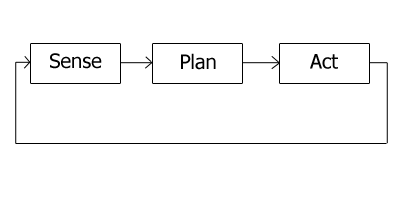
\includegraphics[width=0.5\textwidth]{Figures/Hierarchical.png}
%	\caption{Paradigma jerárquico o tradicional.}
%	\label{fig:ParadigmHierarchical}
%\end{figure}
\begin{itemize}
	\item Fuerte dependencia de una representación interna del ambiente. 
	\item El tiempo de respuesta es lento comparado con el paradigma reactivo. 
	\item El costo computacional es alto.
	\item Con este paradigma se pueden resolver tareas con algo nivel cognitivo.
	\item Dada la dependencia de una representación del ambiente, la capacidad de predicción es alta.
\end{itemize}

\textbf{Reactivo:} En este paradigma el sensado y la actuación se conectan directamente sin que haya de por medio una planeación, como se muestra en la figura \ref{fig:ParadigmReactive}. Sus características en general son contrarias a las del paradigma jerárquico:
%\begin{figure}
%	\centering
%	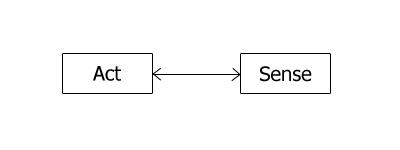
\includegraphics[width=0.5\textwidth]{Figures/Reactive.png}
%	\caption{Diagrama de bloques del paradigma reactivo. }
%	\label{fig:ParadigmReactive}
%\end{figure}
\begin{itemize}
	\item No requiere de una representación del ambiente.
	\item El tiempo de respuesta es rápido comparado con el paradigma jerárquico.
	\item Bajo costo computacional.
	\item En general no es posible resolver tareas que requieran de un alto nivel cognitivo.
	\item La capacidad de predicción es baja. 
\end{itemize}

\textbf{Híbrido:} Tiene como objetivo utilizar las ventajas de ambos paradigmas, es decir, emplear comportamientos reactivos para que el robot responda rápidamente ante cambios en el ambiente sin perder la alta capacidad cognitiva y de predicción que brinda el paradigma jerárquico. La figura \ref{fig:ParadigmHybrid} muestra la forma en que se relacionan las primitivas en este paradigma. 
%\begin{figure}
%	\centering
%	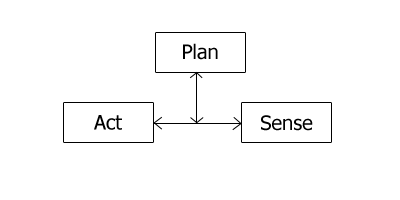
\includegraphics[width=0.5\textwidth]{Figures/Hybrid.png}
%	\caption{Diagrama de bloques del paradigma híbrido.}
%	\label{fig:ParadigmHybrid}
%\end{figure}


%%%%%
%%%%%EL PROBLEMA DE LA PLANEACIÓN DE MOVIMIENTOS
%%%%%
\section{El problema de la planeación de movimientos}
\subsection{Tareas en la planeación de movimientos}
\label{sec:Tasks}

El problema de la planeación de movimientos comprende cuatro tareas principalmente: navegación, cobertura, localización y mapeo. 
Para estas cuatro tareas es necesario tener una descripción o representación de los puntos en el espacio que ocupa el robot. A esta descripción se le llama \textit{configuración} y el \textit{espacio de configuraciones} es el conjunto de todas las configuraciones posibles que puede tener el robot.

La navegación es el problema de encontrar un movimiento libre de colisiones desde una configuración inicial a una final. La cobertura se refiere al problema de mover un sensor o una herramienta de modo que se asegure que se cubren todos los puntos de un espacio determinado. La localización consiste en determinar la configuración del robot dado un mapa y un conjunto de lecturas de los sensores. El mapeo consiste en la exploración y sensado de un ambiente desconocido de modo que se obtenga una representación de dicho ambiente que sea últil para alguna de las otras tareas. Al problema de la localización y mapeo simultáneos se le conoce como SLAM (por sus siglas en inglés). 

En este curso se abordarán únicamente las tareas de navegación y localización. 

\subsection{Características del robot}
Para poder construir un planeador de movimientos es necesario conocer primero las características del robot a utilizar. La primera de ellas es el número de \textit{grados de libertad} que se refiere al número de parámetros independientes que definen la configuración del robot. En el caso de un robot móvil que sólo se mueve en el plano se tienen tres grados de libertad: dos coordenadas de posición $(x,y)$ y una orientación $\theta$. Los espacios de configuración pueden describirse empleando variedades y los grados de libertad definen la \textit{forma} de dicha variedad.

Otra característica importante son las restricciones de movimiento. Si el robot se puede mover en cualquier dirección en el espacio de configuración (en ausencia de obstáculos) se habla de un robot omnidirecciones. Si existen restricciones de velocidad, como en el caso de un automóvil que sólo se puede desplazar en la dirección en la que apuntan las llantas delanteras, entonces se habla de un robot con restricciones \textit{no holonómicas}. Es importante aclarar que una restricción es no holonómica cuando sólo se puede representar en términos de velocidades pero no de posición, por ejemplo, un robot diferencial sólo se puede mover con una velocidad perpendicular al eje que une las llantas, sin embargo, con la planeación adecuada, es posible alcanzar cualquier configuración. El caso contrario es la restricción de movimiento al plano $XY$ que se puede expresar como $\dot{z}=0$ (en términos de la velocidad) o como $z=Cte$ (en términos de la posición).

Finalmente, es importante tomar en cuenta si el modelo del robot será dinámico o solamente cinemático. En el primer caso las señales de entrada pueden ser fuerzas o pares y en el segundo se asume que las velocidades se pueden manipular arbitrariamente y por lo tanto pueden considerarse como señales de entrada. 

\subsection{Características de los algoritmos}

Una vez que se ha definido la tarea a realizar y con base en las características del robot, puede elegirse un algoritmo para resolver determinado problema. Si lo que nos interesa es que el robot ejecute una terea en un tiempo mínimo, con el menor gasto de energía posible o recorriendo la distancia más corta, entonces se requiere de un algoritmo \textit{óptimo}. 

El \textit{costo computacional} de un algoritmo se refiere a la cantidad de recursos necesarios para resolverlo, es decir, cantidad de memoria y tiempo de ejecución. La complejidad se expresa como función de la cantidad de datos de entrada y se suele clasificar como exponencial, polinomial, logarítmica, factorial, etc, dependiendo de la función que pueda acotar ya sea el peor caso o un promedio de los distintos casos. Los datos de entrada pueden ser el número de grados de libertad o el número de estados en un planeador, por ejemplo. 

Otra característica importante de los algoritmos es su \textit{completitud} (se empleará esta palabra a falta de una mejor traducción del vocablo \textit{completeness} en inglés). Se dice que un algoritmo es completo si garantiza encontrar la solución al problema si es que ésta existe. Algunas veces, para disminuir la complejidad de un algoritmo se maneja una completitud para una resolución dada, es decir, el algoritmo garantiza encontrar una solución si se maneja un cierto nivel de discretización. Un ejemplo de esto se verá en la sección \ref{sec:AStar}, en el que una ruta se puede calcular sólo si el espacio navegable se discretiza. 

Una última característica que está más relacionada con la implementación del planeador que con los algoritmos en general, es aquella que se refiere al momento en que se realiza la planeación. Si el planeador construye un plan previo a la ejecución se dice que éste es \textit{fuera de línea}. Si el planeador actualiza el plan conforme lo ejecuta, entonces se dice que es \textit{en línea}.

%%%%%
%%%%% PLANEACIÓN DE RUTAS
%%%%%
\section{Planeación de rutas}
\label{sec:PathPlanning}
\subsection{Celdas de ocupación}

El primer paso para resolver la tarea de navegación es la planeación de una ruta con base en un mapa construido previamente. Como se mencionó en la sección \ref{sec:Tasks}, un mapa es una representación del ambiente que contiene información útil para tomar decisiones. En este curso se emplerán mapas basados en \textit{celdas de ocupación}. En esta representación, el espacio se discretiza con una resolución determinada y a cada celda se le asigna un número $p\in[0,1]$ que indica su nivel de ocupación. En un enfoque probabilístico este número se puede interpretar como la certeza que se tiene de que una celda esté ocupada. 
%\begin{figure}
%	\centering
%	\begin{subfigure}{0.4\textwidth}
%		\centering
%		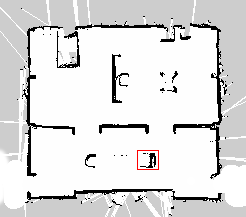
\includegraphics[width=0.8\textwidth]{Figures/OccupancyGrid.png}
%		\caption{A pesar de ser una discretización, con una buena resolución la representación puede ser bastante exacta. Este es un mapa obtenido con el Robot Justina.}
%	\end{subfigure}
%	\hspace{0.05\textwidth}
%	\begin{subfigure}{0.4\textwidth}
%		\centering
%		
\includegraphics[width=0.8\textwidth]{Figures/UniversumZoom.png}
%		\caption{Parte del mapa ampliada donde se aprecia la discretización: las partes blancas son celdas libres, las negras, ocupadas y las grises, aquellas sin información.}
%	\end{subfigure}
%	\caption{Ejemplos de celdas de ocupación.}
%	\label{fig:OccGrids}
%\end{figure}

\subsection{El algoritmo A*}
\label{sec:AStar}
Si se tiene un mapa del ambiente con celdas de ocupación, el problema de la planeación de rutas se puede resolver aplicando un algoritmo de búsqueda en grafos. En este caso cada celda representa un nodo en el grafo y se considera que está conectada únicamente con aquellas celdas vecinas que pertenezcan al espacio libre. Para determinar los nodos vecinos se puede utilizar conectividad cuatro u ocho.

A* es un algoritmo de búsqueda que explora la ruta con el menor costo esperado. Para un nodo $n$, el costo esperado $f(n)$ se calcula como 
\[f(n) = g(n) + h(n)\]
donde $g(n)$ es el costo de la ruta desde el nodo origen hasta el nodo $n$ y $h(n)$ es una heurística que determina \textit{un} costo que se esperaría tener desde el mismo nodo $n$ hasta el nodo objetivo. Este costo esperado de hecho subestima el valor real, es decir, se debe cumplir que $h(n) \leq g(n)\quad \forall\; n \in\; Grafo$. 

En la búsqueda por A* se manejan dos conjuntos principales: la \textit{lista abierta} y la \textit{lista cerrada}. La lista abierta contiene todos los nodos que han sido visitados pero no expandidos y la cerrada, aquellos que han sido visitados \textit{y} expandidos (también llamados nodos conocidos). El algoritmo \ref{alg:AStar} muestra los pasos en pseudocódigo para implementar A*. 
%%\begin{algorithm}
%	\DontPrintSemicolon
%	\KwData{Grafo (celdas de ocupación), nodo inicial, nodo meta}
%	\KwResult{Ruta óptima expresada como una secuencia de nodos}
%	Cerrado $\leftarrow \emptyset$\;
%	Abierto $\leftarrow$ \{nodo\_inicial\}\;
%	previo(nodo\_inicial) $\leftarrow \varnothing$\;
%	\While{ Abierto $\neq\emptyset$ }
%	{
%		nodo\_actual $\leftarrow$ nodo con el menor valor $f$ del conjunto $Abierto$\;
%		Abierto $\leftarrow$ Abierto - \{nodo\_actual\}\;
%		Cerrado $\leftarrow$ Cerrado $\cup$ \{nodo\_actual\}\;
%		\If{nodo\_actual es nodo\_meta}
%		{
%			Anunciar éxito y salir de este ciclo\;
%		}
%		\ForEach{nodo\_vecino de nodo\_actual}
%		{
%			\If{nodo\_vecino $\in$ Cerrado}{Continuar con el siguiente nodo\_vecino}
%			\eIf{nodo\_vecino $\in$ Abierto}
%			{
%				costo\_temporal $\leftarrow g(\textrm{nodo\_actual}) + d(\textrm{nodo\_actual, nodo\_vecino})$\;
%				\If{costo\_temporal $<$ g(nodo\_vecino)}
%				{
%					$g(\textrm{nodo\_vecino})\leftarrow$ costo\_temporal\;
%					$f(\textrm{nodo\_vecino})\leftarrow$ costo\_temporal + heurística(nodo\_vecino, nodo\_meta)\;
%					previo(nodo\_vecino) $\leftarrow$ nodo\_actual\;
%				}
%			}
%			{
%				$g(\textrm{nodo\_vecino})\leftarrow g(\textrm{nodo\_actual}) + d(\textrm{nodo\_actual, nodo\_vecino})$\;
%				$f(\textrm{nodo\_vecino})\leftarrow g\textrm{nodo\_vecino})$  + heurística(nodo\_vecino, nodo\_meta)\;
%				previo(nodo\_vecino) $\leftarrow$ nodo\_actual\;
%				Abierto $\leftarrow$ Abierto $\cup$ \{nodo\_vecino\}\; 
%			}
%		}
%	}
%	\eIf{nodo\_actual $\neq$ nodo\_meta}
%	{
%		Anunciar falla\;
%	}
%	{
%		RutaOptima $\leftarrow\emptyset$ \;
%		\While{nodo\_actual $\neq\varnothing$ }
%		{
%			\textit{//El nodo actual se inserta al principio de la ruta}\;
%			RutaÓptima $\leftarrow$ \{nodo\_actual\} $\cup$ RutaÓptima \;
%			nodo\_actual $\leftarrow$ previo(nodo\_actual)\;
%		}
%		Regresar RutaÓptima
%	}
%	\caption{Búsqueda con A*}
%	\label{alg:AStar}
%\end{algorithm}

\subsection{Suavizado por descenso del gradiente}

Dado que la ruta que arroja A* se calcula a partir de celdas de ocupación, las vueltas siempre serán ángulos rectos, en caso de que se haya utilizado conectividad cuatro, o bien vueltas a $45^o$, en caso de que se haya utilizado conectividad ocho. En cualquier caso, no es deseable tener ``esquinas'' en las rutas por varias razones: la primera de ellas es que la función de posición no es diferenciable en dichas esquinas y, además, este tipo de vueltas ocasionan cambios bruscos en las señales de control, lo que finalmente ocasiona daños a los actuadores del robot. Por otro lado, las restricciones de movimiento en algunos tipos de bases (como es el caso de los automóviles) pueden impedir ejecutar vueltas en ángulo recto.

Por lo anterior, es conveniente suavizar la ruta calculada por A* de modo que la nueva ruta sea lo suficientemente parecida a la original pero al mismo tiempo, lo suficientemente suave para evitar curvas muy pronunciadas. La figura \ref{fig:Smooth} muestra un ejemplo de suavizado con dos casos extremos: la ruta roja es una ruta igual a la original, la azul es una ruta sin vueltas pero que ha dejado de ser una ruta útil, y la verde, que es un \textit{promedio ponderado} de las dos anteriores. 

Para poder obtener una ruta como la verde de la figura \ref{fig:Smooth}, plantearemos una función de costo que tome en cuenta el parecido con la ruta original y el \textit{nivel de suavizado} que se desee. Estos dos criterios están en conflicto: entre más suavizado, menor será el parecido con la ruta original y viceversa, es decir, la función de costo será grande con mucho suavizado y también debe ser muy grande si la ruta es muy parecida a la orignal. La idea es que dicha función de costo tenga un mínimo en un punto intermedio de modo que este punto corresponda a una ruta como la verde de la figura \ref{fig:Smooth}. 

Las funciones cuadráticas son una buena opción como función de costo ya que tienen un mínimo global y además son diferenciables. Para el suavizado de la ruta se propone la función de costo
\begin{equation}
V = \frac{1}{2}\alpha\sum_{i=1}^{n}\left(p_i - q_i\right)^2 + \frac{1}{2}\beta\sum_{i=1}^{n-1}\left(p_i - p_{i+1}\right)^2
\label{eq:Cost}
\end{equation}
donde $Q = \{q_1\dots q_n\}$ son todos los puntos $q = [x\,y]$ que forman la ruta original calculada con A* y $P=\{p_1\dots p_n\}$ son los puntos de la ruta ya suavizada. La constante $\alpha \geq 0$ es un parámetro de diseño para indicar cuánto peso se le quiere dar al parecido de la ruta original con la suavizada y $\beta \geq 0$ indica el peso que se le da al suavizado en sí. Con $\alpha = 0$ se obtendría una línea recta, como la ruta azul de la figura \ref{fig:Smooth}, y con $\beta = 0$ se obtendría una ruta igual a la original.

%\begin{figure}
%	\centering
%	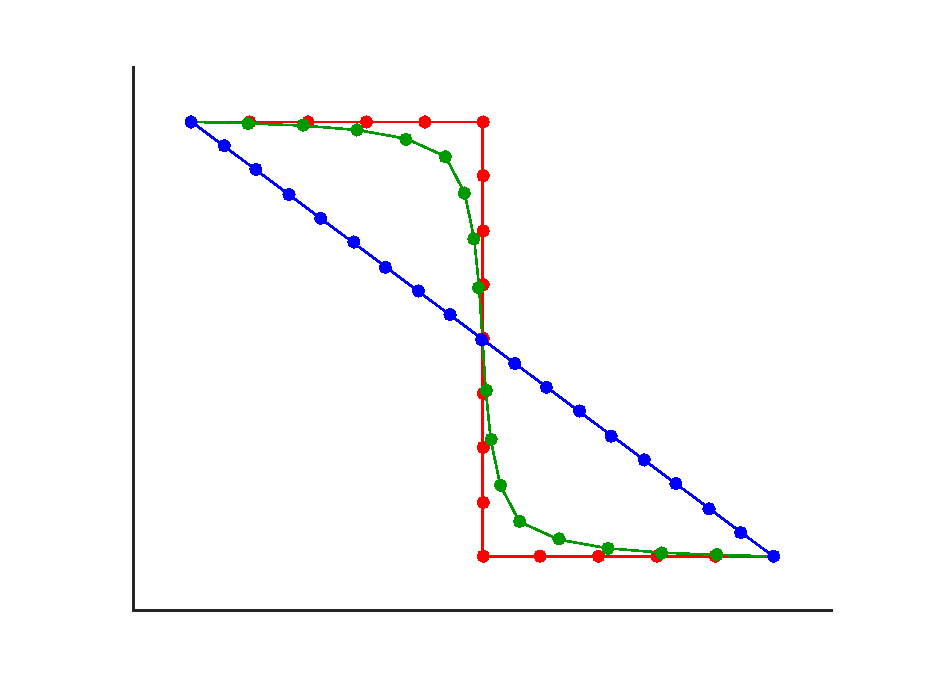
\includegraphics[width=0.5\textwidth]{Figures/Smooth.eps}
%	\caption{Ejemplos de suavizado}
%	\label{fig:Smooth}
%\end{figure}

La ruta suavizada se obtiene encontrando el argumento que minimiza la función \ref{eq:Cost}, sin embargo, dada la cantidad tan grande de variables, es difícil encontrarlo analíticamente. Una forma más sencilla es mediante el médoto del descenso del gradiente, que consiste en mover el argumento pequeñas cantidades proporcionales al gradiente de la función $V$ y en sentido contrario a éste. Dado que el cambio entre cada iteración es proporcional a $\nabla V$, se puede asumir que cuando el cambio en el argumento es menor que una tolerancia, entonces se ha alcanzado el mínimo. 

El algoritmo \ref{alg:Gradient} contiene los pasos en pseudocódigo para implementar descenso del gradiente. La constante $\delta > 0$ debe ser lo suficientemente pequeña para evitar inestabilidad en el algoritmo, sin embargo, se debe considerar que entre más pequeña sea ésta, mayor será el costo computacional. 

\begin{algorithm}
	\DontPrintSemicolon
	\KwData{Función $V$ cuyo mínimo se desea encontrar, condición inicial $p(0)$, tolerancia $tol$.}
	\KwResult{Argumento $p$ que minimiza $V$.}
	$i = 0$\;
	$p_i \leftarrow p(0)$\;
	\While{ $\Vert\nabla V(p_i)\Vert > tol$}
	{
		\BlankLine
		$p_{i+1} \leftarrow p_i - \delta\nabla V(p_i)$\;
		$i \leftarrow i+1$
		\BlankLine
	}
	Regresar $p_i$
	\caption{Descenso del gradiente.}
	\label{alg:Gradient}
\end{algorithm}

La ecuación \ref{eq:Cost} toma como argumentos las posiciones tanto de la ruta original como de la suavizada, sin embargo, dado que sólo varían los puntos de la nueva ruta, se puede considerar que el gradiente $\nabla V$ está dado por:
%\begin{equation}
%\underbrace{\left[\frac{}{}\alpha(p_1 - q_1)+\beta(p_1 - p_2)\right.}_{\ddfrac{\partial %V}{\partial p_1}}
%,\dots ,
%\underbrace{\frac{}{}\alpha(p_i - q_i) + \beta(2p_i - p_{i-1} - p_{i+1})}_{\ddfrac{\partial %V}{\partial p_i}}
%,\dots ,
%\underbrace{\left.\alpha(p_n-q_n)+\beta(p_n - p_{n-1})\frac{}{}\right]}_{\ddfrac{\partial %V}{\partial p_n}}
%\end{equation}
Nótese que se está derivando con respecto a $p$ (puntos de la ruta suavizada), no con respecto a $q$ (puntos de la ruta original). Recuerde que cada punto de la ruta tiene coordenadas $[x\,y]$, por lo que el descenso de gradiente se tiene que aplicar a ambas coordenadas. 

%%%%%
%%%%% MODELO CINEMÁTICO Y CONTROL DE POSICIÓN
%%%%%
\section{Modelo cinemático y control de posición}
\label{sec:Control}
En la sección \ref{sec:PathPlanning} se explicó el modo en que se puede calcular una ruta desde una configuración inicial hasta una final. El siguiente paso es hacer que el robot en efecto siga dicha ruta y para ello se empleará la teoría de control. 

\subsection{Modelo en variables de estado}
Para poder diseñar una ley control que haga que el robot siga la ruta deseada es necesario primero tener un modelo del robot. Para los fines de este curso, un modelo cinemático es suficiente. 

Considérese un robot diferencial como el de la figura \ref{fig:Coords} en el que la configuración está dada por tres valores $\left[x_r, y_r, \theta_r\right]$. Considerando sólo la parte cinemática y asumiendo que no existe deslizamiento en las llantas, el modelo del robot está dado por
\begin{eqnarray}                                                                                                                        
\dot{x_r} &=& \frac{v_l + v_r}{2}\cos\theta_r\label{eq:Kinematic1}\\                                                                        
\dot{y_r} &=& \frac{v_l + v_r}{2}\sin\theta_r\\                                                                                             
\dot{\theta_r} &=& \frac{v_r - v_l}{L}\label{eq:Kinematic3}                                                                               
\end{eqnarray}
donde $v_l$ y $v_r$ son las velocidades lineales de las llantas izquierda y derecha respectivamente, consideradas como señales de entrada, y $L$ es el diámetro del robot medido de eje a eje de las llantas. Se considera que el centro del robot está en el centro de dicho eje.

Nótese que no se está modelando la parte dinámica del robot, esto es, se considera que el estado del robot está dado por los mismos tres valores $\left[x_r, y_r, \theta_r\right]$ y que las velocidades de las llantas se pueden fijar de manera arbitraria. En realidad, esto no sucede así. La verdadera señal de control es el voltaje que se fija en las terminales de los motores, sin embargo, se puede considerar que las dinámicas tanto eléctrica como mecánica de dichos motores son lo suficientemente rápidas para suponer que un voltaje en el motor se reflejará \textit{rápidamente} en una velocidad angular.

%\begin{figure}
%	\centering
%	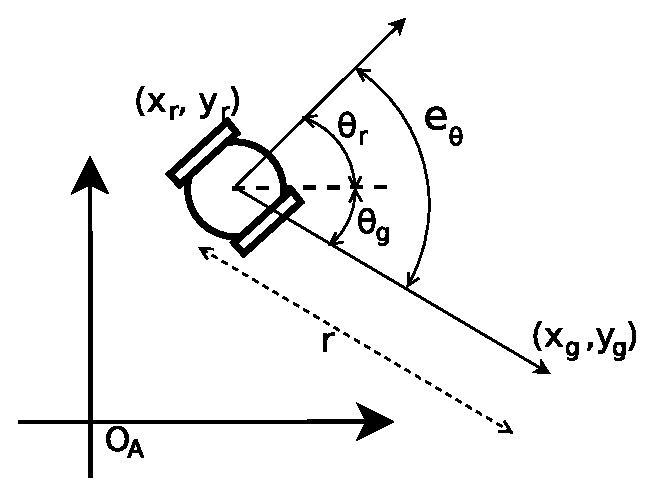
\includegraphics[width=0.5\textwidth]{Figures/GoalPose.eps}
%	\caption{Posición del robot y posición deseada.}
%	\label{fig:Coords}
%\end{figure}


\subsection{Estabilidad de sistemas no lineales}
Cuando se tiene un sistema lineal invariante con el tiempo de la forma
\begin{eqnarray}
\dot{x} &=& Ax + Bu\label{eq:SisLineal1}\\
z &=& Cx + Du\label{eq:SisLineal2}
\end{eqnarray}
es sencillo probar su estabilidad: basta con obtener los valores propios de la matriz $A$ y si todos tienen parte real estrictamente menor que cero, entonces se puede asegurar que el sistema (\ref{eq:SisLineal1})-(\ref{eq:SisLineal2}) es exponencialmente estable, o bien, se puede obtener la función de transferencia equivalente y verificar que todas las raíces del polinomio denominador tengan parte real estrictamente negativa.

Sin embargo, el sistema dado por las ecuaciones (\ref{eq:Kinematic1})-(\ref{eq:Kinematic3}) es no lineal y por lo tanto su estabilidad no se puede analizar con las herramientas descritas en el párrafo anterior. La estabilidad en el sentido de Lyapunov o estabilidad de puntos de equilibrio es una herramienta que nos permite analizar la estabilidad de sistemas no lineales. 

Considérese un sistema dinámico de la forma 
\begin{equation}
\dot{x} = f(x) \label{eq:GeneralSystem}
\end{equation}
donde $x\in R^n$ es el vector de estados. Se dice que $x_e$ es un punto de equilibrio del sistema (\ref{eq:GeneralSystem}) si se cumple que
\begin{equation}
\label{eq:Equilibrium}
x(0) = x_e \implies x(t) = x_e \qquad\forall t > 0
\end{equation}
es decir, si el sistema ``comienza'' en el punto $x_e$, entonces permanece en ese punto para todo tiempo finito.

La estabilidad en el sentido de Lyapunov se define para puntos de equilibrio y existen varios tipos. Para fines de este curso sólo se utilizará la estabilidad asintótica. Suponga que se tiene un sistema de la forma (\ref{eq:GeneralSystem}) con un punto de equilibrio $x_e = 0$. Se dice que $x_e$ es asintóticamente estable, es decir, las trayectorias del sistema convergen a él conforme el tiempo tiende a infinito, si existe una función $V:R^n \rightarrow R$ tal que 
\begin{equation}
V(0) = 0 \qquad\textrm{y}\qquad V(x) > 0 \quad\forall x\neq 0 \label{eq:Lyap1}
\end{equation}
\begin{equation}
\dot{V}(x) < 0 \label{eq:Lyap2}
\end{equation}
La ecuación (\ref{eq:Lyap1}) define a $V$ como una función positivia definida, es decir, como una función escalar de variable vectorial cuyo valor es cero sólo para el vector cero, y estrictamente mayor que cero para cualquier valor diferente de cero. Esta función puede considerarse como una representación de la energía del sistema, solo que expresada en un sistema de coordenadas diferentes a las usuales. 

La equación (\ref{eq:Lyap2}) representa la variación de energía del sistema conforme pasa el tiempo y, si ésta es siempre negativa, significa que la energía siempre disminuirá y en algún momento llegará a cero, es decir, el sistema dejárá de ``moverse''. Esta derivada se tiene que evaluar a lo largo de las trayectorias del sistema (\ref{eq:GeneralSystem}). 

Nótese que se está suponiendo que el sistema tiene un punto de equilibrio en cero, sin embargo, esto no provoca pérdida de generalidad dado que cualquier punto de equilibrio se puede trasladar a cero mediante una transformación de coordenadas. Por otro lado, en la ecuación (\ref{eq:GeneralSystem}) la dinámica sólo es función de los estados y no aparecen señales de entrada, sin embargo, si se diseña un control realimentado, las señales de entrada quedarán en términos de los estados y la dinámica en lazo cerrado podrá expresarse en la forma (\ref{eq:GeneralSystem}). 

Regresando a la aplicación del robot móvil, si se quiere que el robot alcance una posición deseada, las velocidades deben ser tales que el robot tenga un punto de equilibrio asintóticamente estable en dicha posición deseada. 

\subsection{Leyes de control}
La idea del control es diseñar las señales $v_l$ y $v_r$ de modo que se garantice que el robot llegue a la posición $\left(x_g, y_g\right)$ aun en presencia de incertidumbres (como las dinámicas no modeladas) y perturbaciones. Se proponen dos leyes de control para las cuales es necesario definir primero un par de variables.

Considérese el esquema de la figura \ref{fig:Coords}. El ángulo deseado $\theta_g$ corresponde al ángulo del vector de error de posición $\left[x_g - x_r, y_g - y_r\right]$, esto es
\[ \theta_g =  \left(y_g - y_r, x_g - x_r\right)\]
de donde se define el error de ángulo
\[e_{\theta} = \theta_g - \theta_r = \atantwo\left(y_g - y_r, x_g - x_r\right) - \theta_r\]
El error de distancia $r$ es simplemente la magnitud del vector de error de posición:
\[r= \left[\left(x_g - x_r\right) + \left(y_g - y_r\right)\right]^{1/2}\]
En la primera ley de control las velocidades se calculan tomando en cuenta tanto el error de posición como el de ángulo:
\begin{eqnarray}
v_{l} &=& -k_{\theta}e_{\theta} + k_d r e^{-\psi e_{\theta}^2}\label{eq:Control11}\\
v_{r} &=&  k_{\theta}e_{\theta} + k_d r e^{-\psi e_{\theta}^2}\label{eq:Control12}
\end{eqnarray}
Nótese que los primeros términos tienen igual magnitud pero signo opuesto, lo que provoca una velocidad angular que es proporcional al error de ángulo. Los segundos términos, al tener el mismo signo y misma magnitud, provocan una velocidad lineal que es proporcional al error de distancia, es decir, el robot se irá deteniendo conforme se acerque al punto meta. La exponencial sirve para hacer pequeña la velocidad lineal cuando el error de ángulo es grande, es decir, este término logra que el robot comience a avanzar hasta que esté apuntando en la dirección correcta.

En esta ley de control se tienen tres parámetros de diseño: $k_{\theta}>0$, $k_d>0$ y $\psi>0$. Las dos primeras determinan la rapidez con que el robot girará y avanzará hacia el punto meta. La tercera es muy importante. Un valor de $\psi$ muy grande hará que la velocidad lineal decrezca muy rápido cuando crece el error de ángulo, es decir, el robot comenzará a avanzar hasta que esté apuntando casi sin error hacia la meta. Por el contrario, una $\psi$ muy pequeña hará que el robot describa curvas muy grandes.  

La segunda ley de control sólo toma en cuenta el error de ángulo:
\begin{eqnarray} 
v_{l} &=& v_{max}e^{-\frac{e_{\theta}^{2}}{\alpha}} + 
\frac{D}{2}\omega_{max}\left(\frac{2}{1+e^{-\frac{e_{\theta}}{\beta}}}-1\right)\label{eq:Control21}\\
v_{r} &=& v_{max}e^{-\frac{e_{\theta}^{2}}{\alpha}} -
\frac{D}{2}\omega_{max}\left(\frac{2}{1+e^{-\frac{e_{\theta}}{\beta}}}-1\right)\label{eq:Control22}
\end{eqnarray}
En estas ecuaciones se tienen cuatro parámetros de diseño: $v_{max}$ y $\omega_{max}$ son las velocidades lineales y angulares máximas respectivamente que el robot alcanzará durante su movimiento. La constante $\alpha$ tiene una función parecida a la $\psi$ en las ecuaciones (\ref{eq:Control11})-(\ref{eq:Control12}), solo que en este caso, al estar dividiendo, una $alpha$ más pequeña provocará un descenso más pronunciado en la magnitud de la velocidad lineal. El valor de $\beta$ determina qué tanto decrece la velocidad angular conforme decrece el error de ángulo. 


%%%%%
%%%%% CAMPOS POTENCIALES ARTIFICIALES
%%%%%
\section{Campos potenciales artificiales}
En la sección \ref{sec:PathPlanning} se explicó cómo planear una ruta cuando se tiene una representación del ambiente y la seccion \ref{sec:Control} se dedicó al diseño de leyes de control que permitan seguir la ruta planeada. Sin embargo, ¿qué sucede cuando el robot tiene que evadir obstáculos que no están en el mapa y que no fueron contemplados en la planeación de la ruta? 

Un forma de evadir obstáculos es mediante campos potenciales artificiales. Una función potencial es una función real diferenciable $U: R^n \rightarrow R$ que puede verse como una función de energía y que, por lo tanto, su gradiente $\nabla U(q)$, donde $q$ es la posición del robot, representa fuerza. 

El gradiente de la función, dado por
\begin{equation}
\label{eq:PotentialGradient}
\nabla U(q) = \left[\frac{\partial U}{\partial q_1},\dots,\frac{\partial U}{\partial q_n}\right]
\end{equation}
es un vector que apunta en la dirección de máximo cambio de $U$. Si esta función potencial se diseña de modo que tenga un mínimo en la posición meta y máximos locales en la posición de cada obstáculo que se desee evadir, entonces se puede mover al robot mediante el algoritmo de descenso del gradiente y esto hará que el robot continúe moviéndose hasta encontrar un punto $q^*$ en el cual $\nabla U(q^*) = 0$. 

Los valores $q$ que satisfacen $\nabla U(q^*) = 0$ son llamados puntos críticos y pueden ser máximos locales, mínimos locales o puntos silla. Para determinar la naturaleza de un punto crítico, se puede utilizar la matriz Hessiana, dada por

\begin{equation}
\label{eq:Hessian}
H(q) = \left[
\begin{tabular}{ccc}
$\frac{\partial^2 U}{\partial q_1^2}$ &$ \dots$ &$ \frac{\partial^2 U}{\partial q_1 \partial q_n}$\\
$\vdots$ & $\ddots$ & $\vdots$ \\
$\frac{\partial^2 U}{\partial q_n\partial q_1}$ &$ \dots$ &$ \frac{\partial^2 U}{\partial q_n^2}$
\end{tabular}
\right]
\end{equation}

Si $H(q)$ evaluada en $q^*$ es no singular, significa que $q^*$ es un punto crítico aislado. Si $H(q^*)$ es positiva definida, entonces $q^*$ es un mínimo local, si es negativa definida, se trata de un máximo local, y en otro caso, $q^*$ es un punto silla. Si $H(q^*)$ es singular, entonces significa que $q^*$ no es un punto aislado, es decir, que la función potencial $U$ es ``plana'' en la región que contiene a $q^*$. 

En general, si el robot se mueve siempre en sentido contrario al gradiente, en algún momento llegará a un mínimo local. Puede suceder que la condición inicial del robot corresponda a un máximo local o a un punto silla, en cuyo caso el robot no se moverá, pues en estos puntos el gradiente es cero. Esta situación es muy improbable, además, cualquier perturbación hará que el robot ``se mueva'' de ese punto y entonces se dirigirá al mínimo local, es decir, los puntos silla y los máximos son puntos inestables. 

\subsection{Diseño mediante campos atractivos y repulsivos}
Como se expuso previamente, la función potencial $U(q)$ debe diseñarse de modo que sea diferenciable, que tenga un mínimo en el punto meta, máximos locales en cada obstáculo, y todos sus puntos críticos deben ser aislados. Una forma sencilla de logralo es diseñando por separado dos campos: uno atractivo y otro repulsivo. La idea es que el punto meta debe generar una ``fuerza atractiva'' mientras que cada obstáculo debe generar una ``fuerza repulsiva''. 

Algunas veces no es necesario diseñar primero el campo potencial y luego obtener su gradiente, sino que se puede diseñar directamente la fuerza correspondiente al gradiente. La fuerza atractiva se debe diseñar de modo que siempre se aleje del punto meta y las fuerzas repulsivas siempre deben tener una dirección que apunte hacia el obstáculo que se desea evadir, además, las fuerzas repulsivas deben crecer conforme la distancia a dicho obstáculo disminuye y ser muy pequeñas o cero, si el robot está lo suficientemente lejos. 

Es importante recordar que las fuerzas tanto atractiva como repulsiva corresponden al gradiente de la función potencial, es decir, representan la dirección de máximo cambio, sin embargo, lo que se desea es alcanzar un mínimo, por lo que al aplicar el algoritmo de descenso del gradiente, el robot se moverá en sentido contrario a estas fuerzas. 

En este curso, la fuerza atractiva que se utilizará está dada por
\begin{equation}
\label{eq:attractive}
F_a = \zeta \ddfrac{\left(q - q_g\right) }{\Vert q - q_g \Vert}\qquad \zeta > 0
\end{equation}
donde $q$ es la posición actual del robot y $q_g$ es la posición a donde se desea llegar. Esta fuerza tiene una magnitud $\zeta$ constante pero su dirección apunta siempre en sentido contrario al punto meta. 

La fuerza de repulsión está dada por:
\begin{equation}
\label{eq:repulsive}
F_r = \begin{cases}
\eta\left(\sqrt{\frac{1}{\Vert q_{oi} - q\Vert} - \frac{1}{d_0}}\right)\ddfrac{q_{oi} - q}{\Vert q_{oi} - q\Vert}
& \qquad\textrm{si}\quad \Vert q_{oi} - q\Vert < d_0\\
0 & \qquad\textrm{en otro caso}
\end{cases}
\end{equation}
donde $q_{oi}$ es la posición del objeto $i$ y $d_0$ es una distancia de influencia tal que, si el robot está a una distancia mayor que ésta del objeto $i$, entonces la fuerza de repulsión es cero. Nótese que la magnitud de esta fuerza se incrementa conforme el robot se acerca al objeto y la raiz cuadrada produce una transición suave cuando el robot pasa por $d_0$.

La fuerza resultante se calcula como 
\begin{equation}
\label{eq:resulting}
F = F_a + \frac{1}{n}\sum_{i=1}^n F_r
\end{equation}
es decir, la fuerza atractiva más el promedio de las fuerzas repulsivas producidas por cada obstáculo.

Una desventaja de generar campos potenciales mediante la suma de un campo atractivo más uno repulsivo es la posibilidad de tener mínimos locales. Esto se puede solucionar con la generación de funciones potenciales mediante otros métodos como el algoritmo de \textit{wavefront}. Este algoritmo no tiene el problema de los mínimos locales pero tienen la desventaja de necesitar de una discretización del espacio.

\subsection{Movimiento por descenso del gradiente}
Una vez diseñado el campo potencial y calculado el respectivo gradiente, sólo basta con mover al robot de acuerdo con el algoritmo \ref{alg:PotFields}. La constante $\alpha > 0$ debe ser lo suficientemente pequeña para evitar oscilaciones pero sin que ello conlleve un costo computacional muy alto. 

Aunque en el algoritmo se indica que el robot seguirá moviéndose mientras la magnitud del gradiente sea mayor que cero, en una implementación real se fija una tolerancia y cuando la magnitud es menor que ésta, se detiene al robot. 
\begin{algorithm}
	\DontPrintSemicolon
	\KwData{Posición inicial $q_s$, posición final $q_g$, posiciones $q_{oi}$ de los obstáculos}
	\KwResult{Secuencia de puntos $\{q_0,q_1, q_2, \dots\}$}
	$q_0 \leftarrow q_s$\;
	$i \leftarrow 0$\;
	\While{$\Vert\nabla U(q_i)\Vert > 0$}
	{
		$q_{i+1} \leftarrow q_i - \alpha\nabla U(q_i)$\;
		$i \leftarrow i + 1$
	}
	\caption{Descenso del gradiente para mover al robot a través de un campo potencial.}
	\label{alg:PotFields}
\end{algorithm}

Finalmente, para que el robot se mueva hacia cada punto $q_i$ generado por el descenso del gradiente, se pueden utilizar las leyes de control (\ref{eq:Control21})-(\ref{eq:Control22}).

%\section{Conceptos básicos de visión computacional}

%\subsection{Espacios de color}

%\subsection{Operadores morfológicos}

%\subsection{Extracción de planos a partir de nubes de puntos} 

\section{Localización}
El problema de la localización consiste en determinar la configuración del robot dadas las lecturas de los sensores y una representación del ambiente. La localización puede ser global o local. En este curos únicamente se cubrirán dos algoritmos para localizar al robot: el Filtro de Kalman Extendido y el método del histograma. 

\subsection{El Filtro de Kalman Extendido}
El Filtro de Kalman es un algoritmo que sirve para estimar un conjunto de variables a partir de un conjunto de mediciones que contienen ruido y de un modelo del sistema cuyos procesos también contienen ruido. Este filtro puede ser considerado como un filtro bayesiano, pues la estimación de las variables es en realidad la estimación de una distribución de probabilidad conjunta dada una distribución previa y un conjunto de mediciones. 

Desde el punto de vista de la teoría de control, el Filtro de Kalman es un observador en el que la ganancia se calcula con base en las propiedades estadísticas del ruido tanto en las mediciones como en el proceso. 

El Filtro de Kalman Extendido (EKF por sus siglas en inglés) es la versión del Filtro de Kalman para sistemas no lineales. En el EKF se hace una linealización alrededor de las estimaciones actuales y se aplican los mismos pasos que se usan en sistemas lineales. 

Para realizar la estimación de la posición del robot, primero se requiere una versión discreta del modelo cinemático. Discretizando el modelo (\ref{eq:Kinematic1})-(\ref{eq:Kinematic3}), y considerando que se tiene ruido de proceso, se tiene:
\begin{eqnarray}
x_{k+1} &=& x_k + \Delta t \frac{v_l + v_r}{2}\cos\theta_k + \nu_1\label{eq:Discrete1}\\
y_{k+1} &=& y_k + \Delta t \frac{v_l + v_r}{2}\sin\theta_k + \nu_2\\
\theta_{k+1} &=& \theta_k + \Delta t \frac{v_r - v_il}{L} + \nu_3\label{eq:Discrete3}
\end{eqnarray}
donde $\Delta t$ representa el periodo de muestreo y $\nu = \left[\nu_1\;\nu_2\;\nu_3\right]^T$ es ruido gaussiano sin correlación temporal, media cero y matriz de covarianza $Q$. 

La estimación de la posición del robot por filtro de Kalman consta de los siguientes pasos:

\textbf{Predicción:} Con base en el modelo cinemático y el modelo de observación, se predice el siguiente estado y la salida considerando que el ruido es cero tanto en el modelo de transición de estados como en el modelo de obsevación:
\begin{eqnarray*}
	\hat{X}(k+1|k) &=& \hat{F}(X(k|k), u(k))\\
	\hat{Z}(k+1|k) &=& \hat{X}(k+1|k)\\
	P(k+1|k) &=& J(k)P(k|k)J^T(k) + Q
\end{eqnarray*}
donde la matriz $P$ es la covarianza del error de estimación y $J$ es el Jacobiano de la función $F$ con respecto a $X$.

\textbf{Actualización:} Con base en el error de observación y la covarianza del error de estimación se calcula el estado siguiente estimado.
\begin{eqnarray*}
	S(k+1) &=& H(k+1)P(k|k+1)H^T(k+1) + R\\
	K(k+1) &=& P(k+1|k)H^T(k+1)S(k+1)^{-1}\\
	\hat{X}(k+1|k+1) &=& \hat{X}(k+1|k) + K(k+1)(Z(k+1) - \hat{Z}(k+1|k))\\
	P(k+1|k+1) &=& (I-P(k+1)H(k+1))P(k+1|k)
\end{eqnarray*}
donde $H$ es el Jacobiano del modelo de observación, que en este caso es la identidad dado que se considera que se mide el estado completo del robot. La matriz $K$ es conocida como ganancia de Kalman.


\subsection{Método del histograma}
La localización por el método de histograma permite estimar la posición del robot con base en observaciones del ambiente pero tomando en cuenta las probabilidades de error tanto en la observación como en el movimiento. Se asume que el robot sólo puede estar en configuraciones discretas bien definidas por lo que el método es factible sólo cuando se tienen pocos grados de libertad, como en el caso del robot diferencial que se mueve sólo en un plano. 

Considere la posición del robot como un variable aleatoria discreta $X$ que puede tomar los valores $x_i=\{x_1 \dots x_n\}$ y las observaciones que puede realizar el robot como otra variable aleatoria $O$ con posibles valores $o_i=\{o_1 \dots o_m\}$. Las observaciones del robot pueden ser cualquier tipo de \textit{marca} que se pueda extraer a partir de la información de los sensores. 

Se asume que la posición inicial se desconoce por completo, por lo que el primer paso es asignar a cada posición la misma probabilidad
\begin{equation}
P(x_i) = \ddfrac{1}{n}
\end{equation}
es decir, inicialmente se tiene una distribución uniforme que indica total incertidumbre sobre la posición actual del robot. El objetivo es construir una función de densidad de probabilidad que, conforme el robot se mueva y realice observaciones, tienda hacia una distribución unimodal cuyo máximo indique la posición actual del robot.

\textbf{Observación.} 

Para comenzar a estimar la posición del robot es necesario realizar observaciones el ambiente. Para ello, a cada nodo $v$ del grafo $G$ se le asigna una marca que ``debería'' ser observada si el robot se encontrara en ese nodo. 

Con cada observación se debe modificar la probabilidad de cada nodo, dado que se identificó determinada marca. Considérese la posición del robot como una variable aleatoria $V$ que puede tomar los valores $v_i =\left\{\textrm{entrada-izquierda, sala-frente,...}\right\}$ y sea $O = \{o_j\}$ la variable aleatoria que representa la marca observada.


Una vez hecha una observación, se desea actualizar la probabilidad de cada nodo $v_i$, dada la observación $o_j$, esto es
\begin{equation}
P(V = v_i| O = o_j)
\end{equation}
que de acuerdo con el teorema de Bayes se puede calcular como
\begin{equation}
P(v_i| o_j) = \frac{P\left(o_j|v_i\right)P\left(v_i\right)}{P\left(o_j\right)}
\end{equation}
En la ecuación anterior, el término $P\left(o_j|v_i\right)$ es la probabilidad  de que se  observe una determinada marca si se asume que el robot está en el nodo $v_i$, es decir, la probabilidad de $o_j$ en la hipótesis $v_i$. Esta probabilidad se calcula de forma estadística en la etapa de entrenamiento. Si se observa la marca $o_j$ existen dos posibles casos: que la marca corresponda al nodo en el que se asume el robot se encuentra o, que no corresponda. Llamaremos al primer caso un acierto verdadero (AV), y al segundo, un falso positivo (FP). En este trabajo se consideraron las probabilidades
\begin{eqnarray}
P(AV)&=&0.6\\
P(FP)&=&0.25
\end{eqnarray}
El término $P\left(v_i\right)$ denota la probabilidad a priori del nodo $v_i$ y el término $P\left(o_j\right)$ puede calcularse, de acuerdo con el teorema de la probabilidad total, como
\begin{equation}
P\left(o_j\right) = \sum_i^n P\left(o_j|v_i\right)P\left(v_i\right)
\end{equation}
donde $n$ es el número total de nodos del grafo $G$ que representa el ambiente. 

\textbf{Movimiento}
Como se explicó anteriormente, se asume que el robot puede ejecutar tres movimientos: frente, izquierda y derecha. Para modelar la incertidumbre en el movimiento, se asume que existen dos posibles casos: el robot alcanza el nodo deseado o, el robot se queda en el nodo en que ya estaba. Llamaremos al primer caso movimiento correcto (MC) y al segundo, movimiento con falla (MF). Al igual que en el modelo de observación, las probabilidades de ambos casos se calcularon mediante experimentos en la etapa de entrenamiento. Los valores usados fueron:
\begin{eqnarray}
P(MC) &=& 0.7\\
P(MF) &=& 0.3
\end{eqnarray}
Para calcular la probabilidad de cada nodo después de un movimiento, se usa nuevamente el teorema de la probabilidad total. La probabilidad a posteriori de un nodo $v_i$ es la probabilidad de que el robot haya llegado a ese nodo por un movimiento correcto o bien, por un movimiento con falla, es decir
\begin{equation}
P\left(v_i^t\right) = \sum_k P\left(v_i^t|v_k^{t-1}\right) P\left(v_k^{t-1}\right)
\end{equation}
donde los superíndices $t$ y $t-1$ indican el tiempo actual y el tiempo anterior, respectivamente. Si se considera que el robot solo puede llegar a un nodo por un movimiento correcto (viniendo desde otro nodo) o por uno con falla (el robot permanece en el mismo nodo), entonces la ecuación se puede escribir como
\begin{equation}
P\left(v_i^t\right) = P\left(v_i^t|v_k^{t-1}\right)P\left(v_k^{t-1}\right) + P\left(v_i^t|v_i^{t-1}\right)P\left(v_i^{t-1}\right)
\end{equation}
El término $P\left(v_i^t|v_k^{t-1}\right)$ indica la probabilidad de que el robot llegue al nodo $v_i$ desde el nodo $v_k$ (un movimiento correcto), es decir
\begin{equation}
P\left(v_i^t|v_k^{t-1}\right) = P(MC)
\end{equation}
y de modo similar
\begin{equation}
P\left(v_i^t|v_i^{t-1}\right) = P(MF)
\end{equation}


\section{La plataforma ROS}


%-----------------------------------------------------------------------
% Cap�tulo 7
%-----------------------------------------------------------------------
\chapter{Robots Móviles y Agentes Inteligentes}


\section{Máquina de Estado}

\begin{itemize}
	\item[\textbullet] Entradas
	\item[\textbullet] Máquinas
	\item[\textbullet] Salidas
\end{itemize}

\section{Máquina de Estado Aumentada}

Una entrada (o salida) de una máquina puede ser sustituida por la salida de otra máquina de estados. Esa bloquea la entrada (o salida) ordinaria y pone su salida.

\begin{figure}[h!]
	\centering
	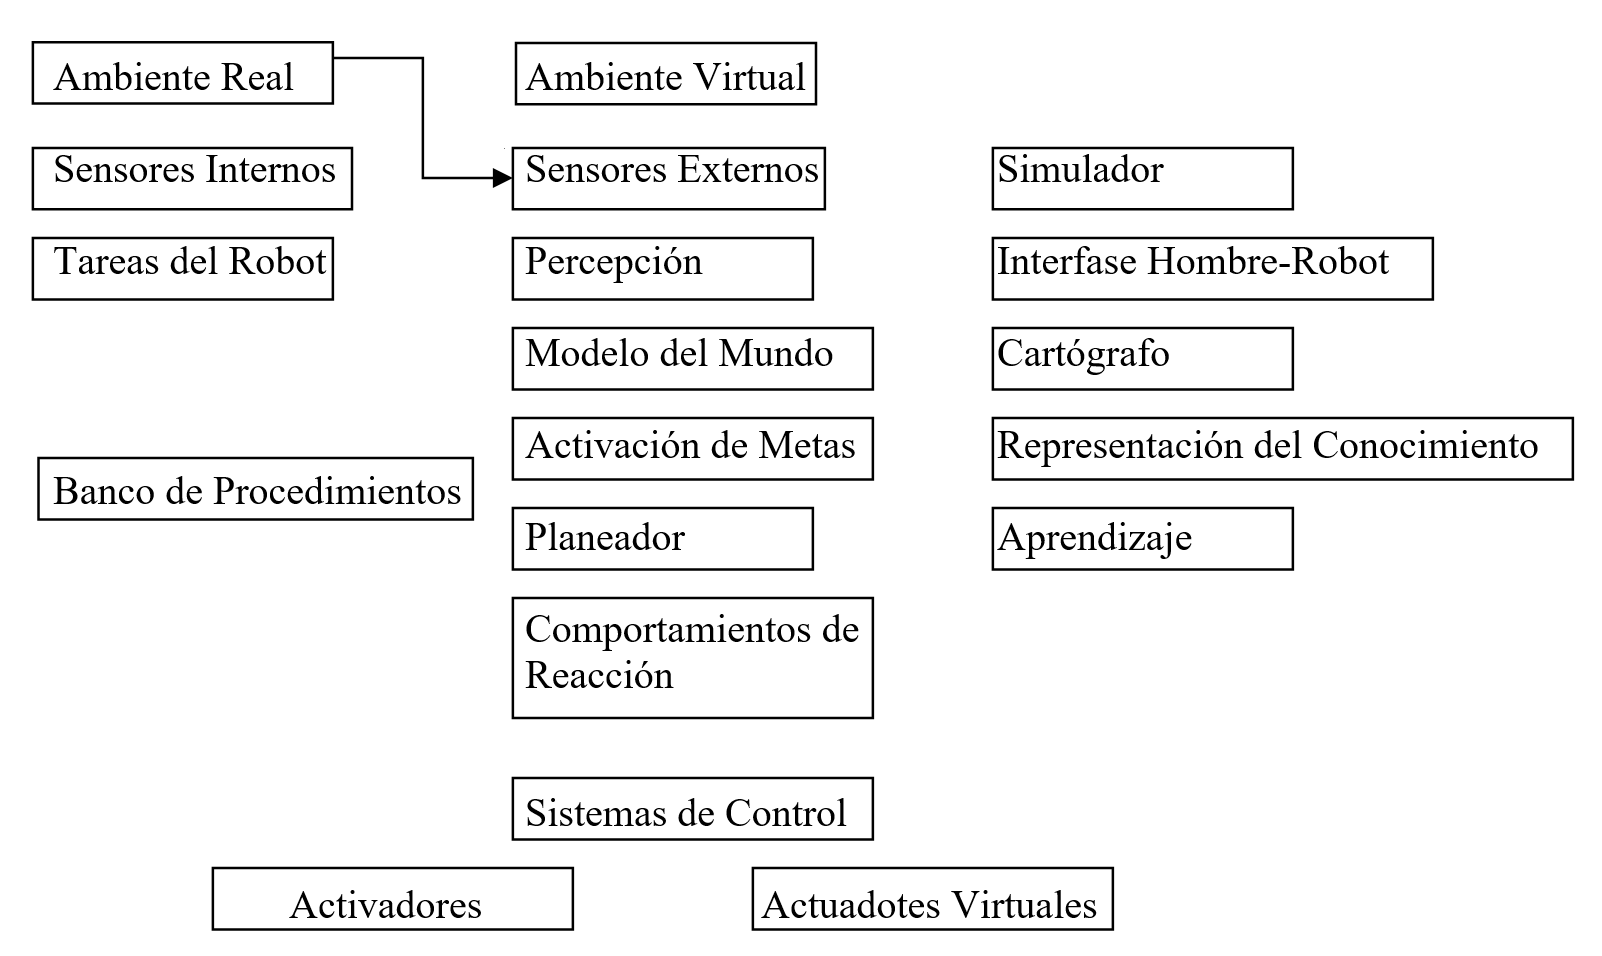
\includegraphics[width=0.5\textwidth]{images/img49.png}
	\label{figura49}
\end{figure}

\section{Arquitecturas Reactivas (o por Comportamientos)}

Diagramas de Stimulus Response (SR)

\begin{figure}[h!]
	\centering
	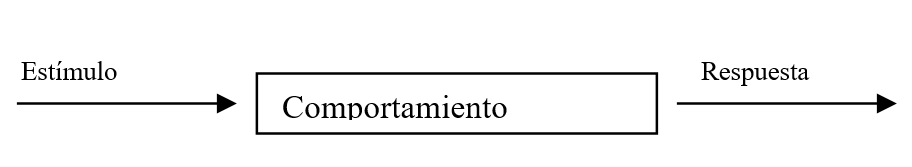
\includegraphics[width=0.5\textwidth]{images/img50.png}
	\label{figura50}
\end{figure}

La idea es que la respuesta sea instantánea.
En los comportamientos puros, la respuesta únicamente depende del estímulo.

\subsection{Organización de los comportamientos:} 

\textit{Esquema 1}

\begin{figure}[h!]
	\centering
	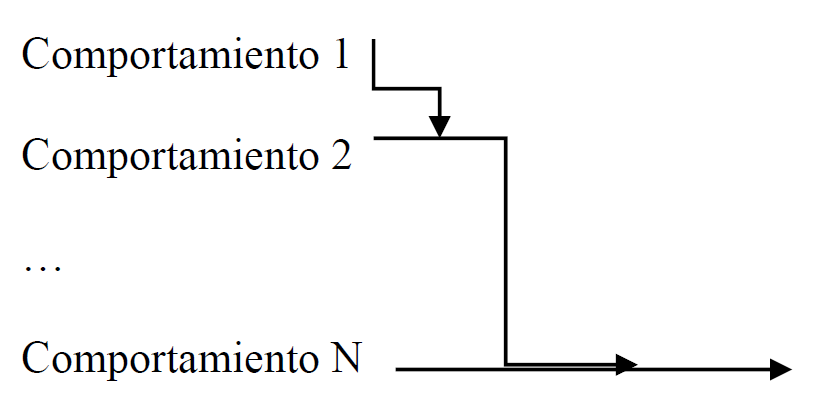
\includegraphics[width=0.5\textwidth]{images/img51.png}
	\label{figura51}
\end{figure}


Algunos comportamientos bloquean la salida de otros. Solamente la salida de uno es el que se usa, todos se activan. El diagrama anterior decide la prioridad.

La salida generalmente es un vector que, por ejemplo, indica la magnitud y dirección del movimiento del robot.

\textit{Esquema 2}

\begin{figure}[h!]
	\centering
	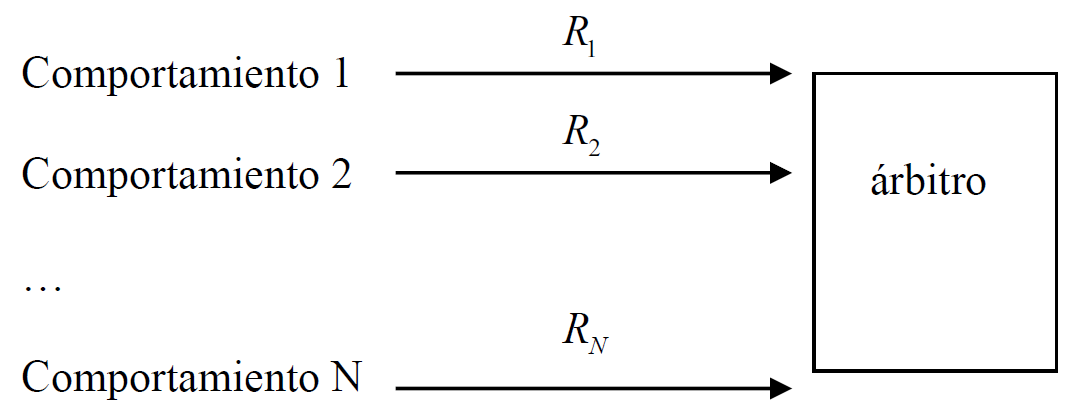
\includegraphics[width=0.5\textwidth]{images/img52.png}
	\label{figura52}
\end{figure}


El árbitro decide cuál es la respuesta.

\begin{figure}[h!]
	\centering
	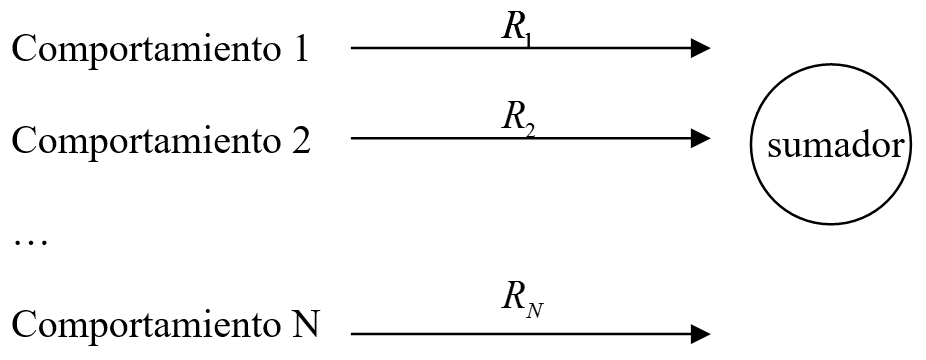
\includegraphics[width=0.5\textwidth]{images/img53.png}
	\label{figura53}
\end{figure}


El sumador hace un promedio ponderado por\textit{ganancias}.

$$
\sum_{i=1}^{N} \, g_i \, R_i
$$

La ganancia depende del diseñador y va a hacer que el robot se comporte de diferente forma (robot “audaz” contra robot “conservador”).

Un diagrama del espacio se puede hacer con campos vectoriales (diagramas de flechitas tipo sistemas dinámicos), por ejemplo uno que sea de las fuerzas de atracción y otro de repulsión y sumarlos.

Puedo tener una complejidad grande combinando comportamientos, pues pueden controlar diferentes cosas.


\section{Máquinas de Estado}
\subsection{Algoritmo para el Comportamiento de Evadir Obstáculos}

Un robot circula con:

\begin{itemize}
	\item[\textbullet] Dos motores, uno a cada lado.
	\item[\textbullet] Dos sensores adelante, para detectar obstáculos (por ejemplo, infrarrojos, ultrasonido, etc.)
\end{itemize}

\begin{figure}[h!]
	\centering
	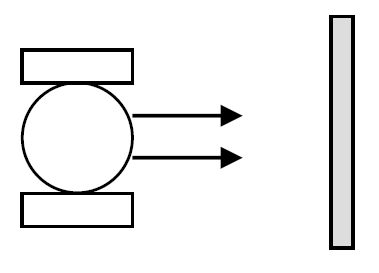
\includegraphics[width=0.5\textwidth]{images/img54.png}
	\label{figura54}
\end{figure}

Obviamente:
\begin{itemize}
	\item[\textbullet] Si los sensores no detectan el obstáculo, seguir 		avanzando.
	\item[\textbullet] Si el sensor derecho lo detecta y el otro no, hacerlo tantito para atrás y girar hacia la izquierda para seguir avanzando
	\item[\textbullet]Si el sensor izquierdo lo detecta y el otro no, hacerlo tantito para atrás y girar hacia la derecha para seguir avanzando
	\item[\textbullet]Si los dos detectan, hacerlo para atrás y giro 90°.
\end{itemize}

\begin{figure}[h!]
	\centering
	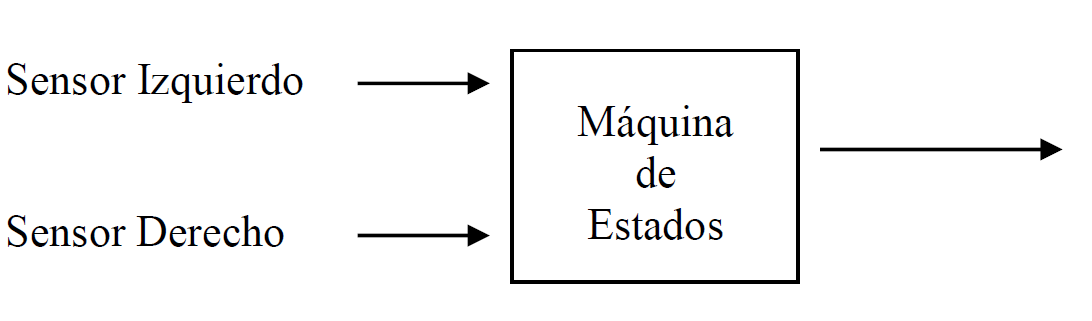
\includegraphics[width=0.5\textwidth]{images/img55.png}
	\label{figura55}
\end{figure}


\textit{Notación de diagrama de flujo}


\begin{figure}[h!]
	\centering
	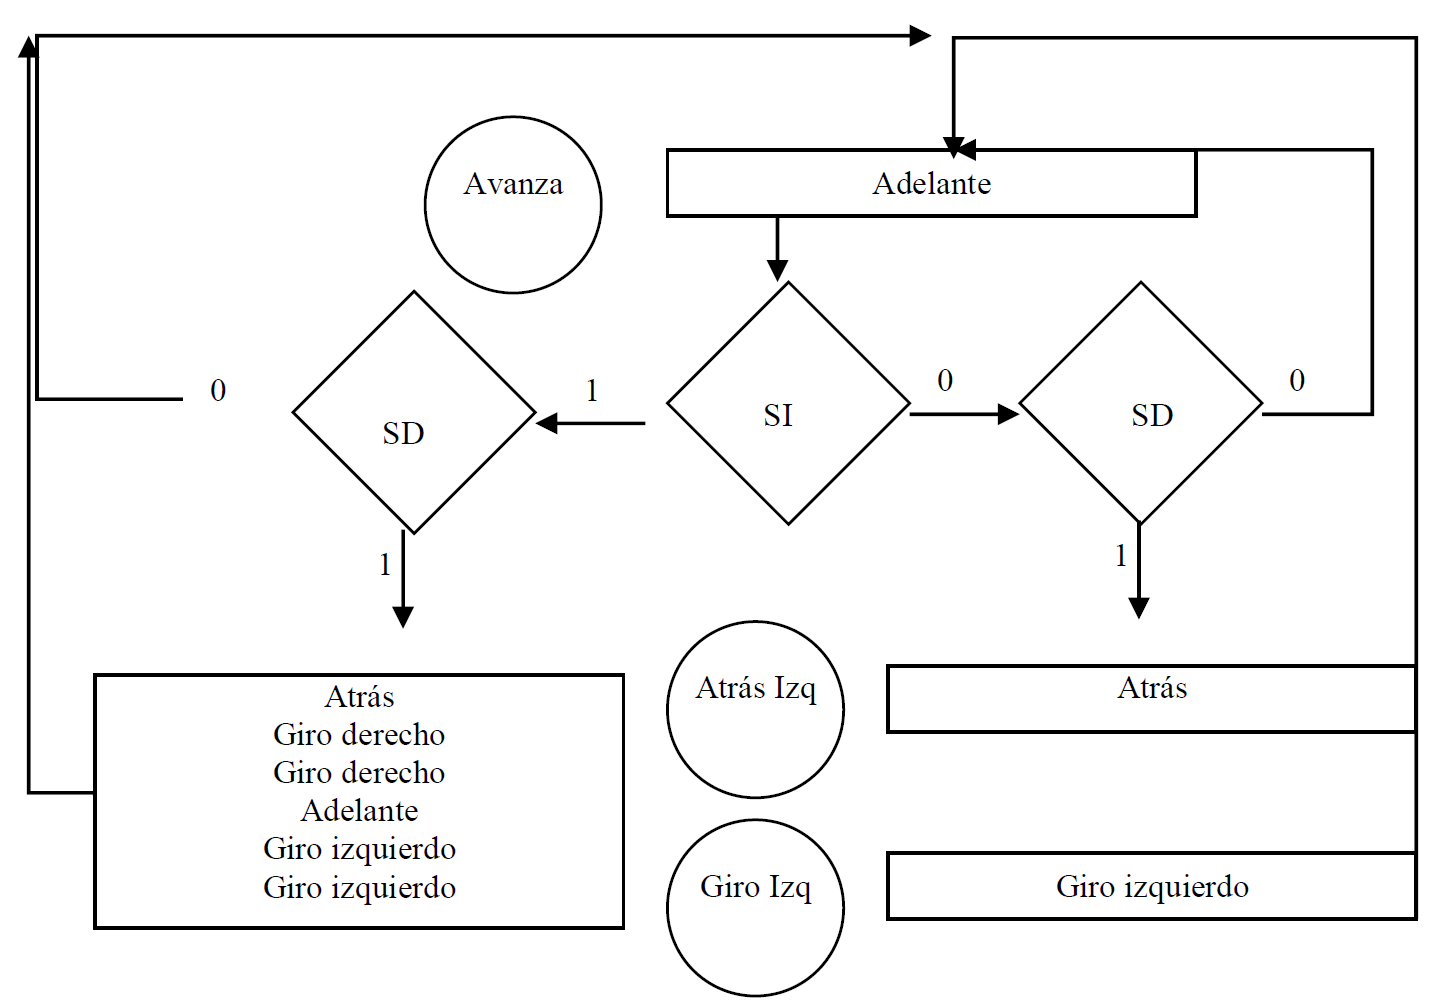
\includegraphics[width=0.5\textwidth]{images/img56.png}
	\label{figura56}
	
\end{figure}
\break

Si se quisiera programar esto con una subrutina, hace todo.  En la teoría de comportamientos necesito una respuesta inmediata y necesito que cuando vuelva a entrar se guarde el estado.

\section{AFSM (Augmented Finite State Machine)}

La máquina de estados aplicada a robots representa el comportamiento.
Una máquina tradicional de estados tiene entradas y salidas.
Rodney Brooks (MIT) inventó la máquina de estados finitos aumentada.

Básicamente el concepto es que alguna de las entradas es inhibida por otra máquina de estados (su salida se convierte la entrada) y en las salidas están los supresores, que bloquean la salida de la máquina y colocan un valor. Por último hay una entrada de “reset” que hace que se coloque en un estado en específico.

Con AFSM podemos tener diferentes capas y hacer una respuesta \textbf{jerárquica}.

\begin{figure}[h!]
	\centering
	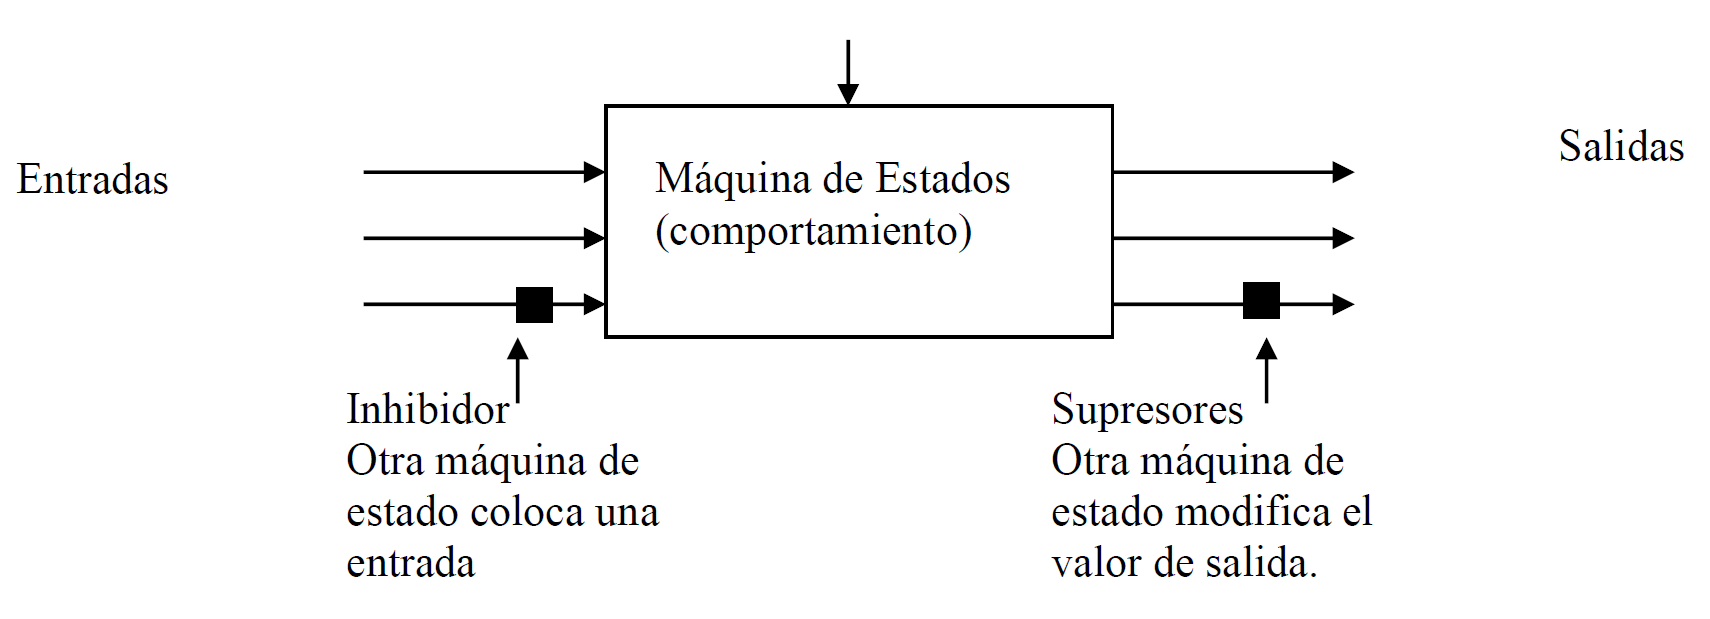
\includegraphics[width=0.5\textwidth]{images/img57.png}
	\label{figura57}
	
\end{figure}
\break

\section{Campos Potenciales}

Se modela el robot como una canica. Los obstáculos ahora son montañas que ejercen fuerzas de repulsión. El destino es un hoyo.
El robot se mueve a través de un campo potencial por la pendiente más pronunciada hasta que lo lleva al destino.

\begin{figure}[h!]
	\centering
	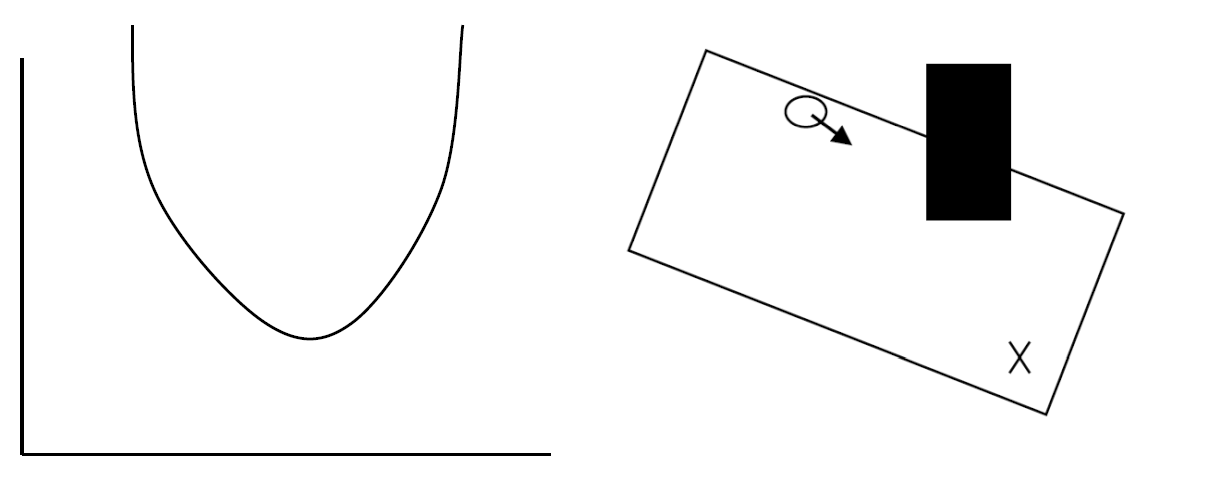
\includegraphics[width=0.5\textwidth]{images/img58.png}
	\label{figura58}
\end{figure}

$$
y=y_0 + (x-x_0)^2
$$


El mínimo se encuentra diferenciando.
$$
\dfrac{\partial y}{\partial x} = 2(x-x_0)
$$
$$
x^* = x_0
$$

Supongamos que no se conoce la ecuación; entonces se utiliza un método iterativo.
Empiezo con un punto $x_{n-1}$ cualquiera y dependiendo del valor de la pendiente me muevo hacia la izquierda o la derecha.

Es una relación de recurrencia:

\begin{center}
	$ x_n= \int(x_{n-1}) = x_{n-1} - \partial \dfrac{\partial y}{\partial x} $ \,  donde $\partial$ es una constante.	
\end{center}

\textbf{Por ejemplo:} \\
Si consideramos $\delta = \dfrac{1}{2}$ se tiene $x_n = x_{n-1} \, \dfrac{-1}{2}(2(x_{n_1}-x_0)) = x_0$.


Esto da pie a considerar la situación general.

\textbf {Se utiliza Steepest Descent.} 

\textit{Posición del robot en n:} $q_n = \left[x_n,y_n\right]^T$
$$
q_n=q_{n-1}-\delta f (q_{n-1}) $$

donde $f(z)= \dfrac{F(z)}{\|F(z)\|} = U(z)$ y $U(z)$  es el campo potencial del medio ambiente en donde navega el robot $U(z)= U_{atr}(z) + U_{rep}(z)$ (dos componentes, uno atractor y un repulsor).

Al final se tienen fuerzas de atracción más fuerzas de repulsión.

Se define:

$U_{atr} = \dfrac{1}{2} \, \varepsilon_1 \,  \|q-q_{dest}\|^2 $(campo de tipo parabólico) donde $q_{dest}$  es la posición del destino. 
Se ve claro que es parabólico:

$$
U_{atr}=\frac{1}{2} \, \varepsilon_1(x-x_{dest})^2 + (y-y_{dest})^2
$$
La fuerza de atracción en q es:

$$
\nabla U_{atr}= \varepsilon_1 \begin{bmatrix}(x-x_{dest}) \\ (y-y_{dest}) \end{bmatrix} = \varepsilon_1[q-q_{dest}] = F_{atr}(q)
$$



La fuerza de atracción se va a convertir en aceleración. Para fuerzas muy grandes se transforma en aceleraciones muy grandes. 
Esto no se quiere, por lo que se tiene un umbral. Esta fórmula solamente aplica para $\|q-q_{dest}\| < d_1$.

¿Qué pasa en $\|q-q_{dest}\|>d_1$?

$$
U_{atr}=E_2\|q-q_{dest}\|
$$

Esto es un campo cónico:

$$
U_{atr}=E_2\sqrt{(x-x_{dest})^2 + (y-y_{dest})^2)}
$$

$$
\nabla U_{atr} = E_2 \begin{bmatrix} \dfrac{(x-x_{dest})}{\sqrt{(x-x_{dest})^2+(y-y_{dest})^2}} \\ 
\dfrac{(y-y_{dest})}{\sqrt{(x-x_{dest})^2+(y-y_{dest})^2}}
\end{bmatrix} = \dfrac{E_2}{\rVert q-q_{dest}\lVert}
\begin{bmatrix}
x-x_{dest} \\
y-y_{dest}
\end{bmatrix} = E_2 \dfrac{q-q_{dest}}{\lVert q-q_{dest}\rVert}
$$

Campos Repulsivos

¿Cómo representar el obstáculo? Se podría considerar un solo vector en el centroide, una serie de puntos que ejercen repulsión, etc. Depende del diseñador.

$$U_{rep}(q)=\frac{1}{2}\eta \left( \dfrac{1}{\lVert q-q_{obs}\rVert} - \dfrac{1}{d_0} \right) ^2 $$

Esto aplica cuando $q-q_{obs}$. En caso contrario, se toma como 0. Esto es para que no lo tomes en cuenta si está demasiado lejos.

$$
\nabla U_{rep}(q)=-\dfrac{\eta}{\rVert q-q_{obs}\lVert ^2} \left( \dfrac{1}{\lVert q-q_{obs}\rVert} - \dfrac{1}{d_0} \right)
\left( \dfrac{q-q_{dest}}{\lVert q-q_{dest}\rVert}\right)
 =F_{rep}(q)
$$

En general,

$$
F(q)=F_{atr}(q)+\sum_{i=1}^{n}\, F_{rep}(q)
$$

$$
f(q)=\frac{F(q)}{\|F(q)\|}=\nabla U(q)
$$

$$
q_{i+1}=q_i - \delta_i f(q_i)
$$

\begin{figure}[h!]
	\centering
	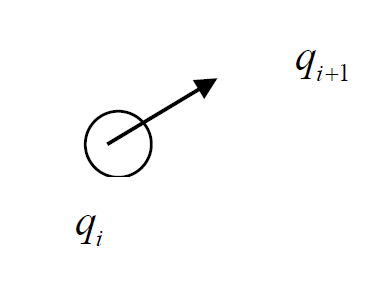
\includegraphics[width=0.3\textwidth]{images/img59.png}
	\label{figura59}
\end{figure}



\begin{ejemplo}
	Robot:(1,1) \\
	Obstáculo: hexágono centrado en (2,2) \\
	Objetivo:(5,4) \\
	$q_0=(1,1)$\\
	Se va a tomar $d_0=	5, \varepsilon_1=1, \eta=2,\delta_0=1$ y se va a utilizar la parabólica
\end{ejemplo}

Se tiene: 

%EJEMPLO
$$
\begin{array}{rcl}
F_{atr}(q_0) & = & \varepsilon_1 (q_0-q_{dest}) \\
             & = &  (-4,-3)
             
             
\end{array}
$$

$$
F(q_0) = - \dfrac{\eta}{\rVert q_0 - q_{obs} \lVert^2} \left(\dfrac{1}{\lVert q_0-q_{obs}\rVert} - \dfrac{1}{d_0} \right)
\left( \dfrac{q_0 - q_{obs}}{\lVert q_0 - q_{obs}\rVert}\right)
$$

$$
= \dfrac {-2}{\sqrt{2}} 
\left(\dfrac{1}{\sqrt{2}} - \dfrac{1}{5}\right) \left(\dfrac{1}{2\sqrt{2}} \right) (-1,-1)
$$


$$=-(0\ldotp3585,0\ldotp3585)$$

La fuerza total es: 



$$
F(q_0) =(-3\ldotp64,-2\ldotp64) \hspace{0.5cm} f(q_0)=(-0\ldotp8091,-0\ldotp 5868)
$$
Finalmente:

%\begin{eqnarray*}
%$$
%q_1 = q_0-\delta_0 (q_0) \\
% = (1,1)+(0\ldotp8091.0\ldotp5868) \\
% = (1\ldotp8091,1\ldotp5868) 
%$$
%\end{eqnarray*}

\begin{equation*}
\begin{aligned}
q_1 & = \,  q_0-\delta_0 (q_0) \\
 & = \, (1,1)+(0\ldotp8091.0\ldotp5868) \\
 & = \, (1\ldotp8091,1\ldotp5868) 
\end{aligned}
\end{equation*}

Obsérvese que no hemos considerado la \textbf{orientación inicial del robot}.



¿Cómo encontrar las constantes? Empíricamente

Nota: Si no conocemos obstáculos no podemos calcular las fuerzas de repulsión. En estos casos, se tiene que usar la información de los sensores para identificar al obstáculo y, con base en eso, calcular estas fuerzas.

\textbf{Cálculo de los vectores de repulsión usando la posición de los obstáculos fijos}

Los obstáculos conocidos se representarán por polígonos que tienen nodos ordenados en el sentido de las manecillas del reloj.

El espacio se divide en celdas y en cada celda se calcula la fuerza total de repulsión.

\begin{figure}[h!]
	\centering
	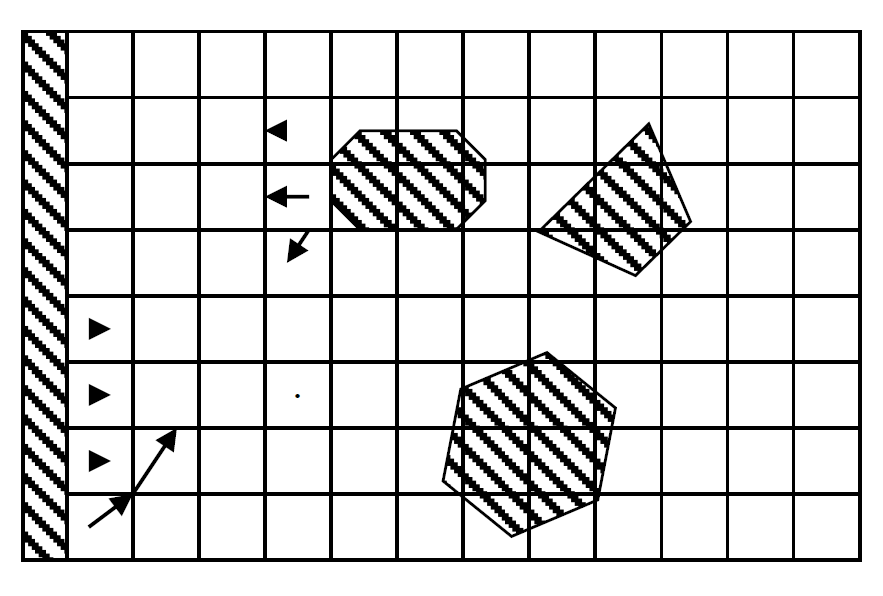
\includegraphics[width=0.5\textwidth]{images/img60.png}
	\label{figura60}
\end{figure}

Etc.

¿Cómo encontrar la fuerza de repulsión en cada celda?

\begin{figure}[h!]
	\centering
	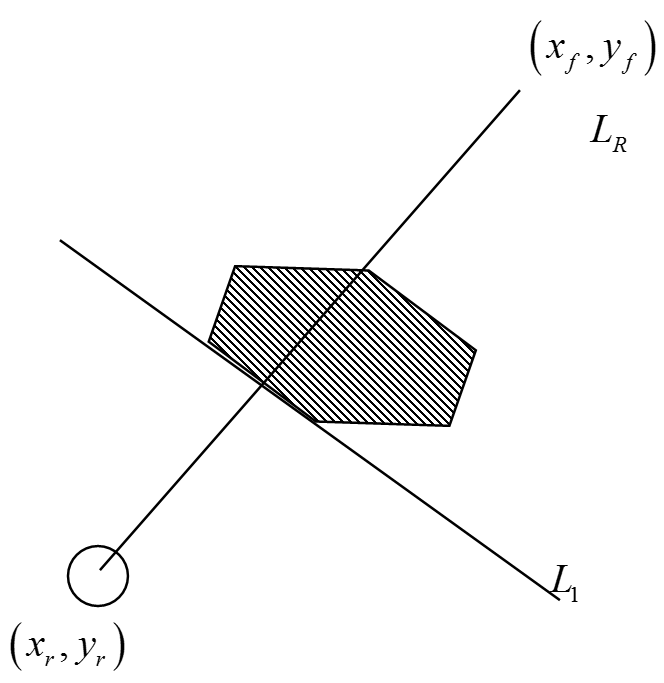
\includegraphics[width=0.5\textwidth]{images/img61.png}
	\label{figura61}
\end{figure}

El punto $x_r,y_r$ es el centro de la celda en donde se está (se asume que el robot está en el centro de la celda).

El punto $(x_f,y_f)$ es  un punto arbitrario (se quiere calcular para la mayor cantidad de direcciones posibles.
No es en línea sino que se hace offline).


\begin{flalign*}
\begin{aligned}
 L_1:\colon y=m_1x+b_1 \\
 L_R:y=m_Rx+b_R
\end{aligned}
\end{flalign*}


Nótese que 

\begin{flalign*}
\begin{aligned}
x_f=d\cos\phi+x_r \\
y_f=d\sin\phi+y_r
\end{aligned}
\end{flalign*}

Donde el ángulo es entre el eje x y la línea $L_R$.

Obs: se puede encontrar

$$
m=\dfrac{y_1-y_0}{x_1-x_0} \hspace{0.5cm} b=\frac{x_1y_0-y_1x_0}{x_1-x_0}
$$

Los puntos de intersección son

$$
x_{int}=\frac{b_r-b_1}{m_1-m_r} \hspace{0.5cm} y_{int}=m_r x_{int} + b_r
$$

Obsérvese que se tiene que cumplir que $x_{int} \in(x_0,x_1)$ y$y_{int} \in(y_0.y_1)$

\section{Cómo calcular el campo potencial para el caso de objetos desconocidos}

Lo anterior se hace offline y se alimenta al robot. Si hay objetos desconocidos:

\begin{figure}[h!]
	\centering
	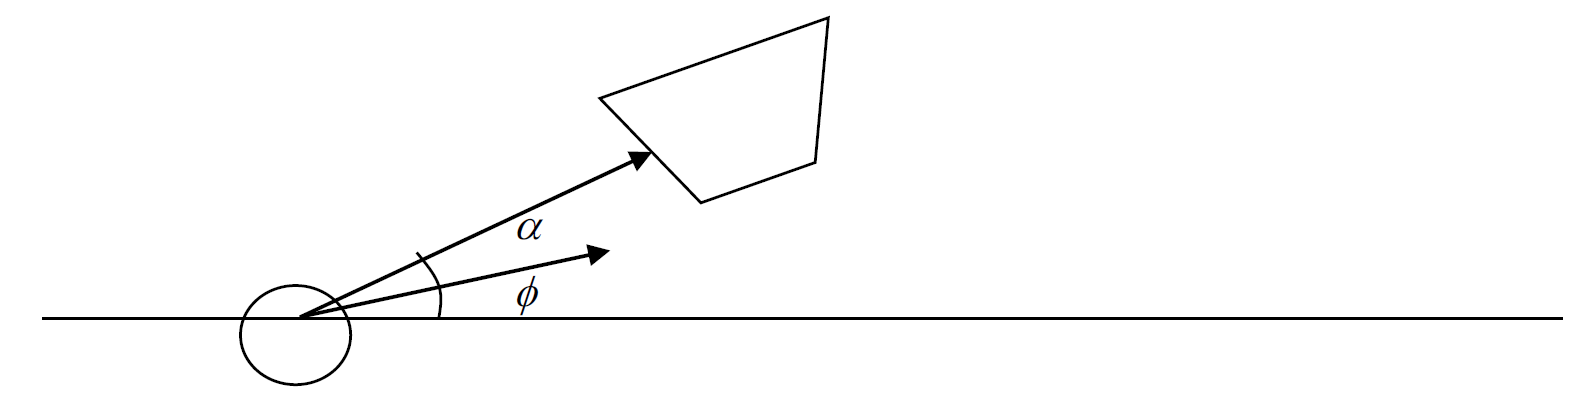
\includegraphics[width=0.5\textwidth]{images/img62.png}
	\label{figura62}
\end{figure}

\begin{scaja}
Tarea 1 \\
Usar Roc2. Poner obstáculos pickable en el medio. Programar un robot para encontrar esos obstáculos y que
los lleve a un lugar. Usar nada más la parte rectangular del mundo. El robot se mueve aleatoriamente. Tener
una pila que se vaya bajando.
\end{scaja}



¿Qué se quiere? \\
De $(x_{i-1},y_{i-1},\phi_{i-|})$ (donde está el robot) necesito llegar a $(x_i,y_i,\phi_i)$.

Obsérvese que: \\
 $x_i=x_{i-1}+x_i \cos(\phi_i)
 y_i=y_{i-1}+x_i \sin(\phi_i)
 $
 
donde:

$
\phi=\phi_{i-1}+\phi_i \\
\phi=\arctan\ (\frac{y_i -y_{i-1}}{x_i -x_{i-1}})
$


Esto se conoce como \textbf{computación directa}.

Otra opción es:

$
x'_i= \dfrac{(x_i - x_{i-1}) + (y_i - y_{i-1})}{\cos(\phi_i) + \sin(\phi_i)}
$

$
\phi_i = \phi_i - \phi_{i-1}
$
y obviamente también se tiene que $x_i = \sqrt{(x_i - x_{i-1})^2 + (y_i - y_{i-1})^2 }$



Esto se llama \textbf{computación inversa} y es la que nos interesa.



\textbf{Ejemplo}



\begin{figure}[h!]
	\centering
	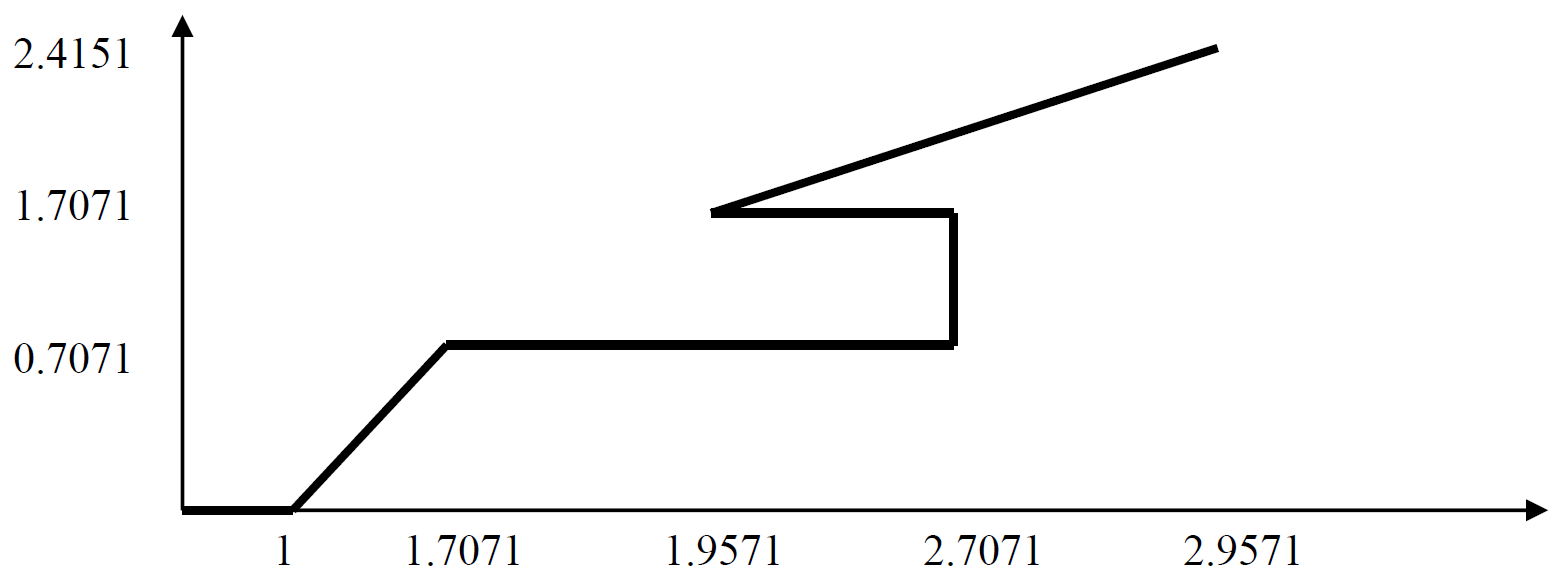
\includegraphics[width=0.5\textwidth]{images/img63.png}
	\label{figura63}
\end{figure}


\underline{Sup:} Los puntos los encontré con campos potenciales (recordar que el campo potencial da el vector de
movimiento:

$q_1=(x_i,y_i) = q_{i-1} - \delta f (q_{i-1})$
\\ \\
$ i=1 $ \\
$ x_0 = 0, \hspace{0.5cm} y_0=0, \hspace{0.5cm} \phi_0=0 $ \\
$x_i =1 \hspace{0.5cm} y_i=0 $

Por lo tanto: $\phi_1 =  arctan \, \left( \dfrac{y_1-y_0}{x_1-x_0} \right) = 0 \hspace{0.3cm} y \hspace{0.3cm} x_1 = \sqrt{(x_1-x_0)^2 + (y_1-y_0)^2} = 1.$ Y finalmente: \hspace{0.3cm} $\phi_i=\phi_i-\phi_{i-1} = 0$

Ad nauseam. \\
Los valores son:

\begin{figure}[h!]
	\centering
	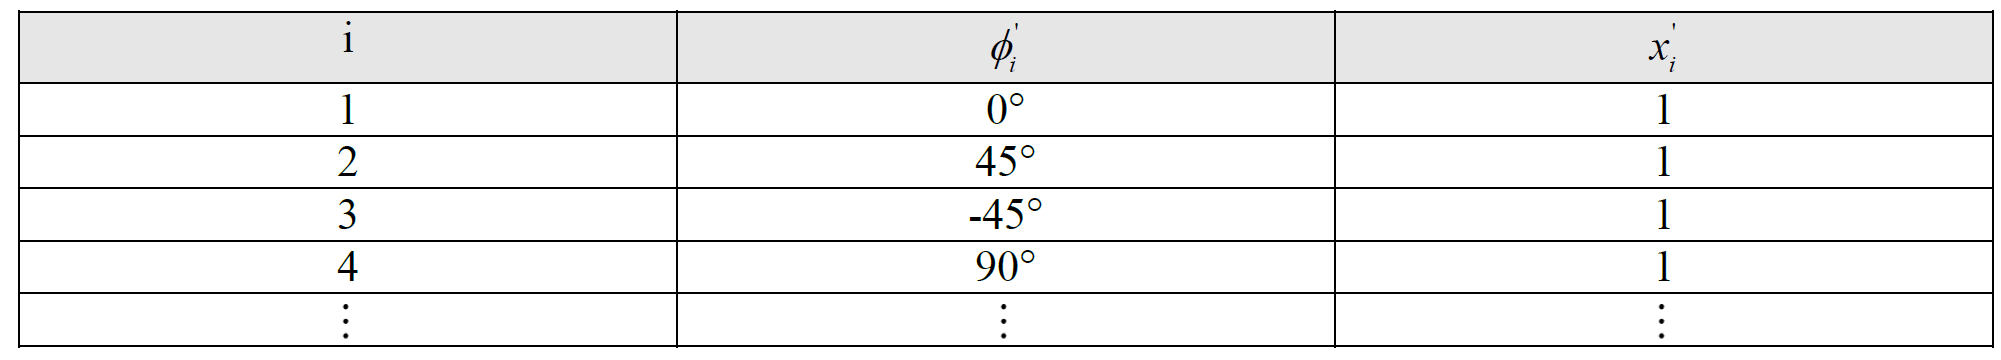
\includegraphics[width=0.5\textwidth]{images/img64.png}
	\label{figura64}
\end{figure}



\subsection{Trayectorias}

El robot casi siempre avanza en línea recta. \\
¿A qué velocidad debe ir el robot?

El robot está en $(x_{i-1},y_{i-1},\phi_{i-1}) $y quiero llegar a $(x_i,y_i)$ .¿Cómo voy a recorrer la distancia $x_i$?
Tengo $t_0$ y el tiempo $t_f$ (final).


\begin{figure}[h!]
	\centering
	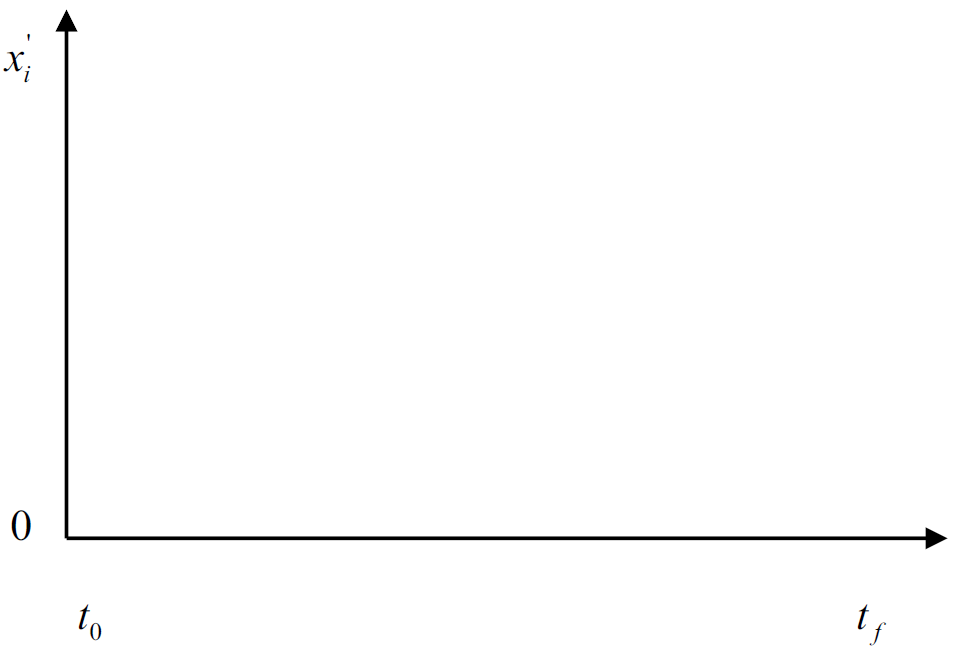
\includegraphics[width=0.5\textwidth]{images/img65.png}
	\label{figura65}
\end{figure}


Se quiere una función $f(t)$ que sea suave. Se asume que el robot está parado en ambos extremos.

$f(0)=0, \, f(t_f)= x_i' \hspace{0.3cm}$ [posiciones inicial y final]

$f'(0)=0, \, f'(t_f)= x_i $ \hspace{0.3cm}[velocidades inicial y final]


Asumiendo una relación cúbica:

$f(t)=a_0 +a_it + a_2 t^2 + a_3 t^3 \, f'(t_f)= x_i$

$f'(t)=a_1 + 2a_2t + 3a_3 t^2$

$f''(t)=2a_2 + 6a_3t$

Se encuentran:

$a_0, a_1=0, a_2=\dfrac{3x_i}{t_f^2},a_2=\dfrac{-2x_i}{t_f^3}$. La ecuación es entonces:
$$
f(t)=\dfrac{3x_i}{t_{f}^2}t^2 - \dfrac{2x'_{i}}{t_{f}^2} t^3
$$

$$
f'(t)=\dfrac{6x_i}{t_{f}^2}t -  \dfrac{6x'_{i}}{t_{f}^2} t^2
$$

$$
f''(t)=\dfrac{6x_i}{t_{f}^2}- \dfrac{12x'_{i}}{t_{f}^2} t
$$

\begin{ejemplo}
	
	
	Suponer $ t_f = 3 \,  x_1=1$ \\
	Entonces
	
	$$f(t)=\dfrac{1}{3}t^2 - \dfrac{2}{27}t^3
	$$
	
	$$f'(t)=\dfrac{2}{3}t - \dfrac{6}{27}t^2$$
	
	$$f''(t)=\dfrac{2}{3} - \dfrac{12}{27}t$$
	
\end{ejemplo}


\begin{figure}[h!]
	\centering
	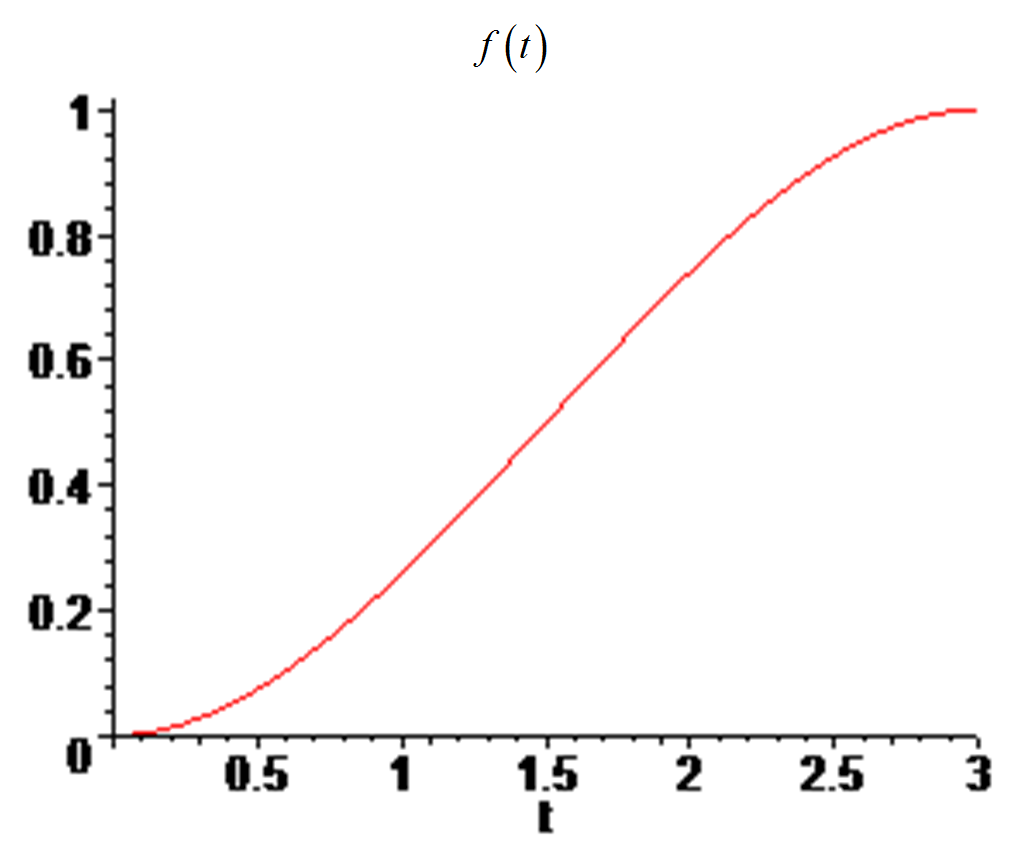
\includegraphics[width=0.5\textwidth]{images/img66.png}
	\label{figura66}
\end{figure}


$$
f'(t)$$
\begin{figure}[h!]
	\centering
	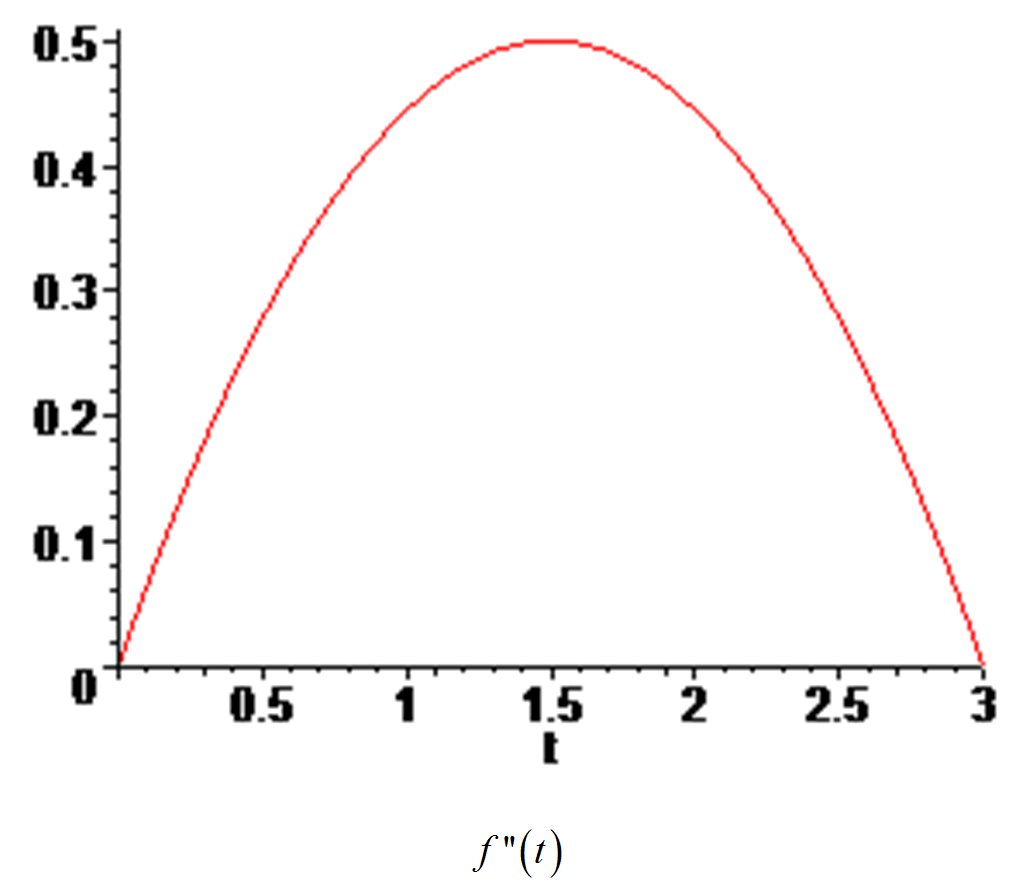
\includegraphics[width=0.5\textwidth]{images/img67.png}
	\label{figura67}
\end{figure}


\begin{figure}[h!]
	\centering
	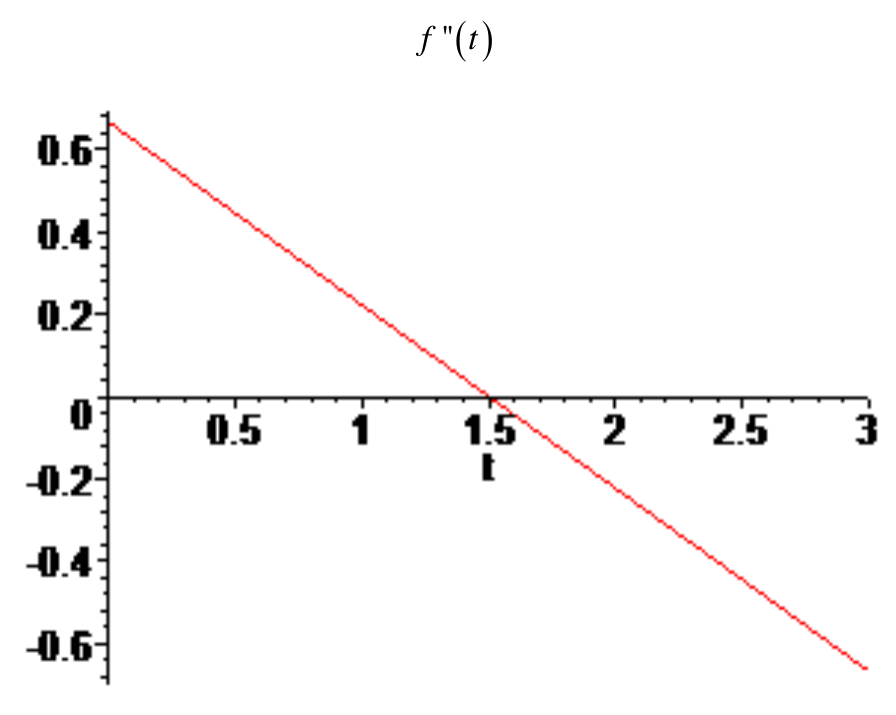
\includegraphics[width=0.5\textwidth]{images/img68.png}
	\label{figura68}
\end{figure}


En Roc2 para mover es:

mv $x'_i \hspace{0.3cm} \phi_i\hspace{0.3cm}t_f$

donde la primera está dada en decímetros y el ángulo en radianes y el tiempo en segundos.

En Roc2 las funciones cinemáticas se encuentran en el archivo Roc2UserMv.

\underline{\textit{Cómo relajar el supuesto de la velocidad final 0}}

Suavizar la trayectoria.

\begin{scaja} 
	
	Una forma: Le ajustas una parábola a la esquinita
	$y=y_0 + (x-x_0)^2$ con $x_b \leq x \leq x_f $ puntos pre-escogidos.
	
	\vspace{5mm}
	
	Otra forma: linearizar (segmentitos de recta).
	
\end{scaja}

\textbf{Rotar y trasladar}

polygon type-object $(x0,  y0, x1, \, y1, \, x2, \, y2, \, ... yn yn)$
position \textit{room} type-object name $xc yc theta ) \leftarrow$ esta función traslada a xc, yc y rota theta
Type-object define un objeto genérico, podemos definir varios objetos (de ese tipo).

\vspace{5mm}
Dados $(x_p,y_p)$


$ x= x_p \cos\alpha - y_p \sin\alpha +x_c $

$y = y_p \cos\alpha + x_p \sin\alpha +y_c$

Donde $x_c$, $y_c$ es el punto fijo sobre el que se está girando.

\begin{ejemplo}
	Polygon mesa $1 \, 0 \, 0\, 0\, 2\, 2\, 2\, 2\, 0$ \\	
	Position salon mesa1 mesa\_principal 44 $\frac{\pi}{4}$
\end{ejemplo}

Entonces:

\begin{figure}[h!]
	\centering
	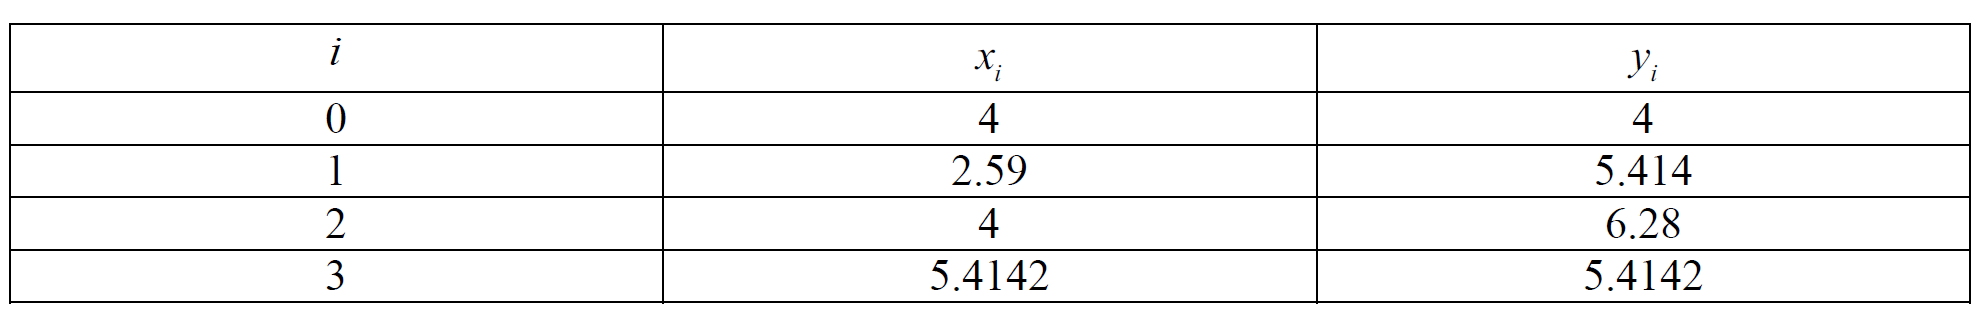
\includegraphics[width=0.5\textwidth]{images/img69.png}
	\label{figura69}
\end{figure}

\textbf{Ancho del robot}
Se necesita considerar el ancho del robot. Por lo menos, ensanchar los obstáculos conocidos en el radio del
robot.
¿Cómo hacer con los desconocidos? De la lectura del sonar, restarle el radio del robot.

\section{Escalamiento de polígonos}

Suponer (0, 2), (1,3), (2, 2), (1,1) un polígono.


\begin{enumerate}[1.]
	\item Encontrar el centroide
	\item Moverlo al origen
	\item Multiplicar
	\item Volverlo a mover al centroide.
\end{enumerate}


Con $\lambda =2$


$P_esc = \lambda (P - C) + C$

$P = \{(-1,2),(1,4),(3,2),(1,0)\}$

\begin{scaja}
	\textbf{Siguiente tarea}
	
	El mundo tiene mesas y otros dos objetos tipo, puestas y rotadas.
	
	Objetos fijos: sillones, mesas, cajas, etc. (al menos 3)
	\\
	
	Descomponer el mundo en celdas.
	\\
	
	Calcular los vectores de repulsión en cada celda.
	Si el centroide de la celda queda dentro del obstáculo, está ocupada
	Hacer una “estrella” hacia todas las direcciones y calcular si la intersección con algo es menor o igual a d0.
	\\
	La repulsión total es la suma.
	\\	
	
	Tres archivos: 1) objetos tipo 2) posiciones objetos réplica 3) archivo final .WRL con la descripción del
	mundo.
\end{scaja}

\textbf{Verificación de si un punto está dentro o fuera de un polígono}

\begin{figure}[h!]
	\centering
	\includegraphics[width=0.3\textwidth]{images/img70.png}
	\label{figura70}
\end{figure}
	%\break

Ecuación paramétrica de la recta
$
x = x_0 + (x_1 - x_0)t \\
y = y_0 + (y_1 - y_0)t \\
t \in (0,1)
$

Los puntos de la ecuación general

$
(y_0 - y_1)x + (x_1 - x_0)y + (x_oy_1 - x_1y_0) = 0
$

Puntos que cumplen esta ecuación, están en la línea.
\\ Puntos que evalúan >0, caen a la izquierda. \\ Puntos que evalúan <0, caen a la derecha.

\textbf{Problema de los campos potenciales}
\\ Por ejemplo un mínimo local


\begin{figure}[h!]
	\centering
	\includegraphics[width=0.3\textwidth]{images/img71.png}
	\label{figura71}
\end{figure}
%\break


El vector resultante es 0 y el robot se queda inmóvil o en un ciclo.

\section{Comportamientos con Redes Neuronales}

Redes neuronales: 1943 $\rightarrow$  McCullock


Una red neuronal es un modelo matemático de cómo funciona una neurona.

Una neurona está conectada a otras neuronas.

\begin{figure}[h!]
	\centering
	\includegraphics[width=0.5\textwidth]{images/img72.png}
	\label{figura72}
\end{figure}

La entrada a la red neuronal es una imagen (por ejemplo, la cámara del robot). Se puede entregar la
información en bruto o procesada.

Las conexiones se van uniendo por medio de aprendizaje.

Se entrena a la red para que siga los comportamientos, por ejemplo un coche autónomo. Para entrenarlo, se
puede poner a un conductor y hacer que la red aprenda los comportamientos de acuerdo a las imágenes.
La respuesta de la red es: para una cierta imagen, se giró a la izquierda violentamente; para otra imagen, se
giró ligeramente; etcétera.

También se puede hacer con información de sonares, etc.

Puedo hacer máquinas de estado con redes neuronales.

\begin{figure}[h!]
	\centering
	\includegraphics[width=0.5\textwidth]{images/img73.png}
	\label{figura73}
\end{figure}

\textbf{Modelo}

Por cada neurona se tiene

$u = \displaystyle \sum_{i=1}^{n} w_i\, y_i + \theta $

Entradas: $ y_j \rightarrow $  vienen de otras neuronas
Pesos: $w_j$
Umbral de activación: $ \theta $

La salida de la neurona es la \textit{función de activación}

$$
a=f(u)
$$

Generalmente $ f(u) = \dfrac{1}{1 + e^\frac{-u}{T}}$ (un sigmoide)

$T$ es una constante de temperatura. 


Resulta que f es la solución de la ecuación diferencial 

$$
\dfrac{dy}{du} = \dfrac{y(1-y)}{T}
$$


\section{Topología de Redes Neuronales}

¿Qué pasa con la topología de redes neuronales (muchas neuronas)?

\begin{figure}[h!]
	\centering
	\includegraphics[width=0.5\textwidth]{images/img74.png}
	\label{figura74}
\end{figure}
\break

Topología acíclica (no hay retroalimentación de la salida hacia otra interna) $\rightarrow$ el dígrafo es acíclico.

\begin{figure}[h!]
	\centering
	\includegraphics[width=0.5\textwidth]{images/img75.png}
	\label{figura75}
\end{figure}


Topología cíclica (con retroalimentación) $\rightarrow$ el dígrafo es cíclico
Estos fueron los primeros modelos de redes neuronales.

\section{Modelo del Perceptrón}

$
u(x) = \sum_{i=1}^{n} w_i x_i + w_0 
$
y

$
y(x) = \begin{cases}
1, \hspace{0.3cm} u(x) \geq 0    \\
0,\hspace{0.3cm}   u(x) < 0  
\end{cases}
$

Este modelo es utilizado para \textit{detección y clasificación}.

Si las características de la entrada $x$ es cercano a $w$ tal que su producto interno $x^Tw$ es mayor que un
umbral $-w_0$, entonces la salida es 1, indicando la detección de un objetivo.


\begin{ejemplo}
	Dos neuronas, una que representa una mesa y otra una silla.
	Las dos tienen las mismas entradas, que son características invariantes a distancia y orientación. La salida
	debe de ser 1 para la de la silla y 0 para la de la mesa.
\end{ejemplo}

\begin{nota} Entrenar a una red neuronal es encontrar los pesos. \end{nota}


Minsky y Shannon

Shannon propone la matemática booleana y notación binaria en las computadoras.
Wiener inventó el término \textit{cibernética} (el estudio de los sistemas – eléctricos, mecánicos, sociales, etc. – y su control).


LEER ASIMOV Y PHILIP DICK

\section{Perceptrón multicapas}

Capa de entradas
Capa intermedia
Capa de salida

\begin{figure}[h!]
	\centering
	\includegraphics[width=0.5\textwidth]{images/img76.png}
	\label{figura76}
\end{figure}

La capa de entrada tiene M neuronas.
La capa intermedia se conoce como \textit{capa oculta} y tiene H neuronas.
La capa de salida tiene N neuronas.

El objetivo es encontrar los pesos que minimicen el error cuadrático medio.


Cada salida de las neuronas de salidas es un objetivo de clasificación.

\begin{ejemplo}
	
¿Cómo encontrar los pesos?

Tres entradas, una neurona de entrada.

$u=Wx$ donde $x = [1 \hspace{0.3cm} x_1 \hspace{0.3cm}  x_2]^T \hspace{0.3cm} y \hspace{0.3cm} W= [W_0 \hspace{0.3cm} w_1 \hspace{0.3cm} W_2]$
\\

Encontrar unos pesos que dado un objetivo $d_k$ e vaya actualizando con la característica que $\varepsilon \rightarrow 0$. Se
tendrán K muestras de entrenamiento $(x_k,d_k)$; salidas $z_k$ y un error total $E= \sum_{i=1}^{K}  \varepsilon_k^2$, donde $\varepsilon= d_k - z_k$.
\\

$d_k \in (0.1)$ generalmente. 

\end{ejemplo}


\begin{figure}[h!]
	\centering
	\includegraphics[width=0.5\textwidth]{images/img77.png}
	\label{figura77}
\end{figure}

Obsérvese que $z_k = f(Wx_k)$.

El objetivo final es minimizar la función $E$ respecto a $W$. 

La solución es no lineal si f es una función sigmoide, por lo que generalmente se realiza la minimización con
iteraciones:

$ W_{t+1} = W_t + \Delta W_t
$

Por método de \textit{steepest descent:}
$\Delta W_t= -\eta \dfrac{dE}{dW}
$

Solución
\\

$$
\dfrac{dE}{dW_i} = -2  \sum_{k=1}^{K}
(d_k - z_k) (\dfrac{-dZ_k}{dw_i})
$$

Obsérvese que

$$\dfrac{-dz_k}{dw_i} = \dfrac{df(u)}{dW_i} = \dfrac{df(u)}{du} \dfrac{du}{dw_i} = f'(u) \dfrac{du}{dw_i} = f'(u) x_i
$$

Por lo que

$$
\dfrac{dE}{dW_i} = 2 \sum_{k=1}^{K} (d_k - z_k) f'(u) x_i
$$

Se denota $\delta_k = [d_k - x_k] f'(u_k)$ y entonces

\begin{scaja}
	$$ w_i(t + 1) = w_i(t) + \eta \sum_{i=1}^{K} \delta_k x_i (k) $$
\end{scaja}

En particular si $f(u)$ es el sigmoide, entonces

$\delta_k=[d_k - z_k] \, z_k \,  (1-z_k)\, \alpha := \dfrac{\partial E}{\partial u}
$

\begin{scaja}
	$$ \dfrac{\partial E}{\partial u} = -2 \sum_{i=1}^{K} [d_k - z_k] \dfrac{dZ_k}{du} $$ y ademas $$\dfrac{dz_k}{du}= \dfrac{f(u)[1 - f(u)]}{T}
	$$.   \\  Por lo tanto, 
	$$
	\dfrac{\partial E}{\partial u} = -2 \sum_{i=1}^{K} [d_k - z_k] f(u) [1 - f(u)] = \dfrac{-2}{T} -2 \sum_{i=1}^{K} [d_k - z_k] \, z_k \, [1-z_k]. 
	$$
\begin{center}
	QED
\end{center}	
\end{scaja}

El proceso se debe hacer hasta que $E\textless \epsilon$


\section{Cómo extender para un perceptrón multicapas}

Se tienen:

K muestras de entrenamiento
L capas

$W_{ij}^L$ es el peso de la neurona $i$ a la neurona $j$ en la capa L y en la iteración $t$.

\textit{Propagación de error:}

\begin{figure}[h!]
	\centering
	\includegraphics[width=0.5\textwidth]{images/img78.png}
	\label{figura78}
\end{figure}

El objetivo es (de nuevo) encontrar $w_ij$ de cada capa que minimicen el error cuadrático medio.

%$$ \dfrac{dE}{dw_ij^L} = -2 \sum_{i=1}^{K} \dfrac{dE}{du_i^L (k)} \dfrac{du_i^L(k)}{dw_ij^} = -2 \sum_{k=1}^{K} \delta_i^L (k) \dfrac{du_i^L(k)}{dw_ij^L}$$

Pero dado que

$
\dfrac{du_i^L (k)}{dw_{ij}^L} = \dfrac{d}{dw_{ij}^L}  \sum_{m=1}^{M} \hspace{0.2cm} w_{im}^L \hspace{0.2cm} z_{m}^{L-1} (k) 
$

%avances hasta hoy 17 

Se puede reescribir la parcial como:

$$\dfrac{dE}{dw_{ij}^L} = -2 \sum_{k=1}^{K}  \delta_{i}^L (k) z_{j}^{L-1}(k)$$
	
Se observa que el error $\delta_i^L$ en esta capa depende del error en la capa anterior, por lo que se necesita utilizar una derivación tipo Bellman para tener:

$$ \delta_{i}^L (k) = \dfrac{\partial E}{\partial u_{i}^L (k)} $$

\begin{figure}[h!]
	\centering
	\includegraphics[width=0.5\textwidth]{images/img79.png}
	\label{figura79}
\end{figure}

Obsérvese que tiene la siguiente recursión:


\begin{equation*}
	\begin{aligned}
		 \delta_i^L (k) & = \, \dfrac{\partial E}{\partial u_{i}^L }(k) = \sum_{m=1}^{M} \dfrac{dE}{du_m^{L+1}} \dfrac{du_m^{L+1} (k)}{\partial u_i^L (k)}  \\
		& = \,\sum_{m=1}^{M} \delta_m^{L+1} (k) \left[ \dfrac{d}{\partial u_i^L (k)} \dfrac{j=1}{J} w_{mj}^L f (u_j^L (k)) \right] \\
		& = \, f'(u_i^L(k)) \sum_{m=1}^{M} \delta_m^{L+1} (k) w_{mj}^L 
	\end{aligned}
\end{equation*}

Esto se conoce como \textit{backward propagation}.

La fórmula de actualización será entonces:
\begin{figure}[h!]
	\centering
	\includegraphics[width=0.9\textwidth]{images/img79_f.png}
	\label{figura79_f}
\end{figure}

La $\eta$ da la velocidad de convergencia. Sin embargo, si es muy grande, se puede dar la situación que se oscile
demasiadas veces antes de llegar al mínimo.
El error aleatorio se suma para encontrar el mínimo global.

\textbf{¿Cómo se usa esto para los robots?}

En Carnegie-Mellon University, se realizó un experimento en el cual un robot pudo manejar 90\% autónomamente en una autopista larga de Estados Unidos.

\begin{figure}[h!]
	\centering
	\includegraphics[width=0.9\textwidth]{images/img80.png}
	\label{figura80}
\end{figure}

El entrenamiento se haría primero manejando un humano y la red registrando qué se hizo y la foto
correspondiente.
Otra forma: máquina de estado con redes neuronales.

\textbf{Máquina de Estados con Redes Neuronales}

\begin{figure}[h!]
	\centering
	\includegraphics[width=0.9\textwidth]{images/img81.png}
	\label{figura81}
\end{figure}


\section{Aprendizaje}

El aprendizaje en un robot puede ser varias cosas:

1. Aprender “audacia”: esto depende de las constantes (afinación de constantes)
Para campos potenciales: $\mu, \delta, d_1, d_0, \eta $.

2. Aprender nuevos comportamientos

a) Crear nuevos algoritmos de máquinas de estado.

b) Modificación de las máquinas de estado \\

Hay dos cosas: una, lo que aprendemos, y otro, el conocimiento que se obtiene a través de la evolución. Por
ejemplo, un bebé sabe cómo evitar un obstáculo, no tiene que aprender. \\



\textbf{\textit{Adquisición de Comportamientos Básicos (evolución)}}

ALGORITMOS GENÉTICOS
Los algoritmos genéticos nos permitirán utilizar el concepto de evolución para:
- Afinación de constantes
- Generación de algoritmos de máquina de estado. \\


\textbf{\textit{Adquisición de Conocimiento Nuevo a partir de Comportamientos Básicos (heredados)}}

REDES NEURONALES
Aprendizaje por medio de ejemplos (tú le enseñas qué debe de hacer en determinadas circunstancias).


\textbf{¿Qué es un algoritmo genético?}

\begin{figure}[h!]
	\centering
	\includegraphics[width=0.9\textwidth]{images/img82.png}
	\label{figura82}
\end{figure}

Las operaciones básicas sirven para evaluar a los individuos, es decir se genera una medida para evaluar a
cada secuencia de bits.
%NOTA no se puede poner imagen :(
%\begin{ejemplo}
% 
%
%	\begin{figure}
% 
% 	\includegraphics[width=0.9\textwidth]{images/img86.png}
% 	\label{figura86}
% 	\end{figure}
% 		
%\end{ejemplo}

\begin{figure}[h!]
\centering
\includegraphics[width=0.9\textwidth]{images/img83.png}
\label{figura83}
\end{figure}
\break 


Ahora suponer que se cruza el individuo 1 con el 2 y tiene dos descendientes:

\begin{figure}[h!]
	\centering
	\includegraphics[width=0.9\textwidth]{images/img84.png}
	\label{figura84}
\end{figure}

Para hacerlo “realista” se tienen que tomar partecitas (bloques de bits) del mismo lugar (por ejemplo del
segundo bloque).

Mutación:

\begin{figure}[h!]
	\centering
	\includegraphics[width=0.9\textwidth]{images/img85.png}
	\label{figura85}
\end{figure}


\textbf{\underline{1. Afinación de Constantes en Campos Potenciales}}

Se tiene un \textbf{cromosoma} que codifica las constantes de un robot que navega usando campos potenciales.

\begin{figure}[h!]
	\centering
	\includegraphics[width=0.9\textwidth]{images/img86.png}
	\label{figura86}
\end{figure}

Por ejemplo si $\mu = 3.5$ y se quiere tener cuatro bits para la parte entera y cuatro para la decimal:

$0011 1000$
Pues es $(0)2^3 + (0)2^2 + (1)2^0 + (1)2^{-1}$

(verificar que esto es cierto)

Si se tienen n individuos y se evalúan en un medio ambiente, la función podría ser:

$$ f(ind_i) = \dfrac{k_1}{d(x_*,f_f)} + \dfrac{k_2}{pasos} + ... + k_n choques $$

\underline{En cada generación se cambia el origen y el destino.}

En la última generación ya se tienen las constantes adecuadas. \\


\textbf{\underline{2. Generación de algoritmos de máquinas de estado}}

Cromosoma que codifica la máquina de estados.

\begin{figure}[h!]
	\centering
	\includegraphics[width=0.9\textwidth]{images/img87.png}
	\label{figura87}
\end{figure}

Cada estado, a su vez, es un conjunto de variables de salida y decisiones (condicionales – “if”s) con las
variables de entradas.



Por ejemplo, el estado 1 se codificaría de la siguiente manera:

\begin{figure}[h!]
	\centering
	\includegraphics[width=0.9\textwidth]{images/img88.png}
	\label{figura88}
\end{figure}

...sigue...

\begin{figure}[h!]
	\centering
	\includegraphics[width=0.9\textwidth]{images/img89.png}
	\label{figura89}
\end{figure}

\begin{ejemplo}
Codificar el estado (1) en: \\
$(1) Var5 = 7 \rightarrow (2)$
\end{ejemplo}

La solución es el binario de:

\begin{figure}[h!]

	\includegraphics[width=0.3\textwidth]{images/img90.png}
	\label{figura90}
\end{figure}

Es decir: 

\begin{figure}[h!]
	
	\includegraphics[width=0.3\textwidth]{images/img91.png}
	\label{figura91}
\end{figure}

\textbf{Ojo}: necesito una máquina que realmente evalúe este cromosoma y lo ejecute como una máquina de estados.

\begin{ejemplo}
	Codificar la máquina: \\
	$ (1) var1 = 3, var4 = 8 \rightarrow 10 < S3 < 25 ? (2) | (18)$
\end{ejemplo}

Solución: el binario de:

\begin{figure}[h!]
	
	\includegraphics[width=0.9\textwidth]{images/img92.png}
	\label{figura92}
\end{figure}

\begin{ejemplo}
Codificar lo siguiente:
\end{ejemplo}


\begin{figure}[h!]
	
	\includegraphics[width=0.8\textwidth]{images/img93.png}
	\label{figura93}
\end{figure}

 



\begin{nota}
LO IMPORTANTE ES QUE EL CROMOSOMA SE PUEDA EJECUTAR. Por ejemplo, si hay
condicionales de ambos lados no se puede con esta estructura.
\end{nota}

\begin{nota}
	Al hacer mutaciones o cruzamientos, hay que tener cuidado. Por ejemplo si se cruzan dos individuos
	de dos estados, y me da uno de un estado, habría que cortar el hijo para que la información posterior nada
	más tenga un estado. Igual si cambia a tres, añadir un estado. O cruzar condicionalmente... por ejemplo si
	cruzo el número de estados, podría tener que cruzar también la información de los estados etcétera.
\end{nota}


\begin{ejemplo}
	Codificar 
	\begin{equation}
	\begin{aligned}
		(1) M1 & = 0\ldotp 5; M2 = 0\ldotp3 \rightarrow 1 \ldotp 0 < S3 < 1\ldotp3 ? \\
		& T: (2) M1 = 0\ldotp1, M2 = 0\ldotp4  3\ldotp1 < S2 < 4\ldotp1 \\
		&\hspace{0.5cm} T: (2) \\
		&\hspace{0.5cm} F: 2\ldotp3 < S5 < 4 ? \\
		&\hspace{1cm}T: (3) M1 = 0\ldotp7, M2 = 0\ldotp7 \rightarrow 6 < S2 < 7\ldotp0 ? \\
		& \hspace{1.5cm} T: (3) \\ 
		& \hspace{1.5cm}F: 2\ldotp1 < S3 < 4\ldotp0 ? \\ 
		& \hspace{2cm}T: (3) \\
		& \hspace{2cm}F: (1) \\
		& \hspace{1cm}F: (2) \\ 
		& F: 3\ldotp1 < S1 < 4\ldotp7 ? \\
		& \hspace{0.5cm} T: (3) \\ 
		& \hspace{0.5cm}F: 1\ldotp1 < S2 < 1\ldotp2 ? \\
		& \hspace{1cm}T: (2) \\
		& \hspace{1cm}F: (1) \\ 
	\end{aligned}
	\end{equation}
\end{ejemplo}


\section{\underline{Utilización de algoritmos genéticos para organizar los comportamientos (arbitraje)}}

%imagen 
\begin{figure}[h!]
	\centering
	\includegraphics[width=0.9\textwidth]{images/img94.png}
	\label{figura94}
\end{figure}

Recuérdese que

$$c_f = \sum_{i=1}^{N} g_i \textbf{b}_i
 $$

donde $g_i$ son las constantes de ganancia y $\textbf{b}_i$ son los vectores de movimiento por los diferentes
comportamientos.

Además se tiene una \underline{función de desempeño global} que indica si el robot cumplió el objetivo.

\begin{itemize}
	\item[\textbullet]Una forma es encontrar las constantes g i con algoritmos genéticos, basándose en la función de
	desempeño global.
	\item[\textbullet]Otra forma de organizar es poniendo prioridades.
\end{itemize}

\subsection{Método de Utilidad Múltiple (Utility Manifold)}
Se quiere que el árbitro decida cuál de los comportamientos se debe activar.
Todos los comportamientos dan salidas siempre.
Cada comportamiento dirá su aplicabilidad, dependiendo de:

\begin{itemize}
		\item[\textbullet]los sensores internos
		\item[\textbullet]los sensores externos
\end{itemize}

Esto es un valor en (0,1)

1. Función de activación del comportamiento

$f_{H_i} (S_I, S_E , V)$

donde 

$S_I$ son los sensores internos (batería, odómetro, etc.)
$S_E$ son los sensores externos (sonares, infrarrojo, etc.) 
$V$ son variables de estado $x_1 ,..., x_r$

Se modela:

$f_{B_i}(S_E, S_I, x) = a_{i0} + a_{i1} S_E + a_{i2} S_I + a_{i3} x_i +  a_{i4} S_E^2 + a_{i5} S_I^2 + a_{i6} x_i^2 + a_{i7} S_E S_I + a_{i8} S_I x_i + a_{i9} S_E x_i ,$ para $i=1,\ldotp \ldotp \ldotp, n$ los $n$ comportamientos

Se quiere obtener $a_{ij}$ con algoritmos genéticos. 

Se definen: 

$ x_i = \begin{cases} b_{i1} + b_{i2} \; e^{-|b_{i3}|t_i}, \hspace{0.3cm} B_i \;$ est\'a activo $ \\
0,\hspace{0.3cm}   e.o.c.  
\end{cases} $	


Para cada comportamiento se tiene una función de activación. Se tienen diferentes individuos y, dentro
del cromosoma, se tiene:



\begin{figure}[h!]
\centering
\includegraphics[width=0.6\textwidth]{images/img95.png}
\label{figura95}
\end{figure}
(en binario)

\begin{scaja}
	Resumen
	Los algoritmos genéticos se utilizan para introducir a los robots los comportamientos básicos. Esto NO corre
	en línea, es para “alambrar” los “instintos” al robot. 
\end{scaja}

\section{Planeación}

¿Cómo planear la ruta de un punto a otro? 

\begin{figure}[h!]
	\centering
	\includegraphics[width=0.6\textwidth]{images/img96.png}
	\label{figura96}
\end{figure}
(en binario)

Se quisiera encontrar camino más rápido.

Supóngase que se tiene un campo potencial y un obstáculo
¿Cómo se podría ajustar los campos potenciales?:

\begin{figure}[h!]
	\centering
	\includegraphics[width=0.6\textwidth]{images/img97.png}
	\label{figura97}
\end{figure}


Una idea podría ser tratar de encontrar \textit{varios} caminos por campos potenciales, dependiendo de un cierto
ángulo de desvío $\theta$.

Esto genera un árbol de opciones (caminos) que es muy costoso recorrer con \underline{fuerza bruta}. ¿Cómo recorremos
este árbol para que sea inteligente?

El objetivo es encontrar una mejor ruta para recorrerla. 

\subsection{Búsqueda de la mejor ruta}

El problema de búsqueda se puede formular como sigue:
 
\begin{scaja}
	Dado
	
	$x_0$ un punto inicial (o nodo)
	$x_f$ un punto objetivo (o nodo)
	un grafo con pesos (red topológica)
	
	se quiere encontrar una ruta óptima que llegue al punto objetivo desde el punto inicial y recorrerla.

\end{scaja} 

\begin{ejemplo}
	
Observe la siguiente imagen 

\end{ejemplo}

\begin{figure}[h!]
	\centering
	\includegraphics[width=0.6\textwidth]{images/img98.png}
	\label{figura98}
\end{figure}

\textbf{Depth-first}

Funciona para árboles

Es necesario convertir la red en árbol. Se ponen únicamente los caminos únicos (no recursivos).
Se ponen los pesos acumulados en cada nivel

Este approach se vuelve gigantesco, por lo que es necesario hacer un approach inteligente:

$\bullet$	Se va a realizar la búsqueda recorriendo el árbol por preorden hasta que sea nulo (en cuyo caso se
saca de la lista y se mete otro hijo del padre) o sea el objetivo.

S \\
A | S \\
B | A | S \\
C | B | A | S \\
E | B | A | S \\
D | E | B | A | S \\
F | E | B | A | S \\
G | F | E | B | A | S \\ 

Aquí ya se encontró el destino por lo que se encontró un camino de nodos. Ésta es la forma de encontrar un
camino.

La aplicación es:

\begin{enumerate}[1.]
	\item El planeador encuentra los nodos del grafo que hay que visitar	
	\item Cada uno se convierte en un punto de atracción sucesivo en el algoritmo de campos potenciales	
\end{enumerate}



\textbf{Hill Climbing}

Tiene una función heurística.
Generalmente la función del costo (o peso) al nodo más la distancia remanente al destino

$f(d(q_j, q_F), w_{ij})$

Es el costo de pasar de un nodo a otro más (por ejemplo) la distancia euclideana en R 3 del punto físico
asociado al nodo y el punto físico asociado al destino.

\textbf{Breadth-Search}

Se va guardando en una lista ligada
En cada iteración se van cargando los hijos de cada uno de los nodos de cada nivel.

\textbf{Planeación usando espacio-estado}

Reglas nombre {
	Precondiciones
	$\rightarrow$
	Operadores
	Lista de Borrado
	Lista Aditiva
}


\textit{Por ejemplo: Ponerse los zapatos:}


Regla Colocar$\_$Calcetin$\_$Derecho
Precondiciones

Colocar Zapato Derecho (comando) \\

Pie derecho está desnudo

Calcetín está disponible

$\rightarrow$

Operador

Poner$\_$Calcetin$\_$PieDerecho

Lista de Borrado

Calcetín está disponible

Pie derecho está desnudo


Regla Colocar$\_$Zapato$\_$Derecho \{
	Precondiciones
	
	No hay pie derecho desnudo
	
	Colocar Zapato Derecho (comando)
	
	Zapato derecho disponible
	
	$\rightarrow$
	
	Operador
	
	Poner zapato derecho
	
	Lista de borrado
	
	Zapato derecho disponible
	
	Colocar zapato derecho
\}



Se pueden organizar jerárquicamente:

Inicio

a) Colocar$\_$Calcetin$\_$derecho \\
a. Colocar$\_$zapato$\_$derecho \\
i. Colocar$\_$calcetin$\_$izquierdo \\
ii. Colocar$\_$zapato$\_$izquierdo \\

b. Colocar$\_$calcetin$\_$izquierdo \\
i. Colocar$\_$zapato$\_$izquierdo \\
1. Colocar$\_$zapato$\_$derecho \\
ii. Colocar zapato derecho \\
1. Colocar zapato$\_$izquierdo \\

b) Colocar$\_$Calcetin$\_$izquierdo\\
a. Colocar zapato izquierdo\\
i. Colocar calcetín derecho\\
ii. Colocar zapato derecho\\

b. Colocar calcetín derecho\\
i. Colocar zapato derecho\\
1. Colocar zapato izquierdo\\
ii. Colocar zapato izquierdo\\

1. Colocar zapato derecho\\


¿Por cuál camino irnos?
Debemos ponerle pesos y después trabajarlo con un algoritmo de búsqueda.


\begin{ejemplo}
	Bloques
	
	B	A	C	E	D
	Se quiere tener una representación espacio-estado con los operadores.
	
	B	D	C 	E	A
	
	
\end{ejemplo}

Operadores:


Goto(x,y,z) \hspace{0.5cm} Ir a (x,y,z) \\
Pickup(w) \hspace{0.5cm}Recoger w de la mesa \\
Putdown(w) \hspace{0.5cm}Soltar w en la mesa \\
Stack(u,v) \hspace{0.5cm}Poner el u encima del v \\
Unstack(u,v) \hspace{0.5cm} Quita el bloque u del v (y se lo queda en la mano)


La representación del estado del mundo:


Location(w,x,y,z) \hspace{0.5cm}  el bloque w está en las  coordenadas x,y,z \\
On(x,y) \hspace{0.5cm} el bloque x está encima de y \\
Clear(x) \hspace{0.5cm} no hay algo encima de x \\
Gripping(x) \hspace{0.5cm} el brazo del robot tiene el bloque x \\ (\textit{gripping(void)} es que no tiene algo) \\
OnTable(w) \hspace{0.5cm} el bloque w está en la mesa


A partir de esto se deduce que

$$\forall x (CLEAR(x)) \Rightarrow \neg \exists y (on(y,x)))$$
$$\forall x (GRIPPING (void) \Leftrightarrow \neg GRIPPING (x)$$
$$\forall y \forall x (ONTABLE (y) \Rightarrow \neg ON (y , x ))$$


Estado 1

	OnTable(A)\\
	OnTable(C)\\
	OnTable(D)\\
	On(B,A)\\
	On(E,D)\\
	Gripping(void) \\
	Clear(B) \\
	Clear(C) \\ 
	Clear(E)\\ 


Regla Pickup(x) \{
	Precondiciones \\
	Clear(x) \\
	OnTable(x) \\
	Gripping(void) \\
$\rightarrow$
	Lista de adición \\
	Gripping(x) \\ 
	Lista de borrado \\
	OnTable(x) \\
	Gripping(void) \\
\}


Observación: esto genera una \textit{notación de predicados}
 
$$ \forall x (PICKUP (x) \Rightarrow GRIPPING (x)) \leftarrow (GRIPPING (void) \textasciicircum CLEAR (x) \textasciicircum ONTABLE (x))
$$

Regla PutDown(x) \{ \\
	Precondiciones \\
	Gripping(x) \\
	$\rightarrow$
	Lista Adición \\
	Gripping(void) \\
	OnTable(x) \\
	Lista de Borrado \\
	Gripping(x) \\
\}

Regla Stack(x,y) \{ \\
	Precondiciones \\
	Gripping(x) \\
	Clear(y) \\
	$\rightarrow$ 
	Lista de adición \\
	Gripping(void) \\
	On(x,y) \\
	Lista de Borrado \\
	Gripping(x) \\
	Clear(y) \\
\}

Árbol de Estados

B A
C E
D


1) B
A E
C D

2)


A E
C D


Etcétera (todas las posibilidades)

\underline{Tercera evaluación}

Comportamiento de potenciales
Comportamiento de máquinas de estado
Árbitro


(con variables de aplicabilidad entre 0 y 1)



\textbf{Máquina de Inferencia}


Hechos + Reglas $\rightarrow$ Máquinas de Inferencia $\rightarrow$ Agenda
Los hechos activan reglas. Las reglas pueden generar otros hechos que, a su vez, pueden activar nuevas
reglas.

Por ejemplo esto puede evitar que en 100000 if’s anidados se tenga que ejecutar el último.
En lugar de que las reglas busquen los hechos que los activan, es al revés (puesto que los hechos
generalmente no cambian).


Las reglas producen hechos NUEVOS.

El sistema \textbf{CLIPS} es un lenguaje de programación orientado a plantillas que permite definir sistemas
expertos. Tiene una máquina de inferencia con encadenamiento hacia delante para eficiencia.
Permite definir hechos, reglas, etc.


\section{Lenguaje Natural}

La idea es hablarle a un robot en lenguaje cotidiano y que nos “entienda”. Entender es hacer un análisis
semántico para obtener un significado y transformarlo en una acci
ón.

Lo que yo le dije, que lo haga.

La definición operacional de \textbf{entender} es que el sistema realice las acciones que el usuario le pide.
Entender algo es transformar lo que se pide en una \textbf{representación}, la cual ha sido escogida para que
corresponda a un conjunto de acciones disponibles que pueden ser ejecutadas.


\begin{enumerate}[1.]
	\item Señal de entrada \\
	Puede ser voz, imagen o combinación de ambas (o cualquier otra forma de entrada, por teclado).
	Voz: por medio de un micrófono que transforma una señal acústica en una señal eléctrica.
	Es necesario aplicar técnicas de procesamiento digital de señales para obtener las características de
	esa señal acústica.
	Existen algoritmos (como el de cuantización vectorial y sus variantes) para procesar e identificar las
	palabras.
	
	\item Las palabras de entrada son revisadas para ver si ellas están agrupadas de acuerdo con reglas
	gramaticales, significando que ellas forman oraciones gramaticalmente correctas.
	
	\item El significado de cada palabra y de la oración es asignado.
	Este paso es el más difícil de los tres.
	
\end{enumerate}



\textit{Dependencia Conceptual}

\underline{Primitivas Conceptuales}

La representación de varias acciones es la misma.
Por ejemplo: “Juan dio el libro a Pedro”, “Juan prestó el libro a Pedro”, “Juan regaló el libro a Pedro”,
significan cosas diferentes, pero la acción de transferir el libro de una persona a otra es la misma.

Cada primitiva tiene:

\begin{enumerate}[a)]
	\item Un actor (realiza el acto)
	\item Un acto (realizado por el actor y hecho hacia un objeto)
	\item Un objeto (ente sobre el que es realizada la acción)
	\item Una dirección (en la cual el acto es realizado)
	\item Un estado (en el cual el objeto se encuentra)
\end{enumerate}

Las primitivas son:

\textbf{PTRANS} \hspace{0.5cm}
Es la transferencia física de un objeto. 

\hspace{2cm}
(PTRANS (Actor NIL) (Objeto NIL) (FROM NIL) (TO NIL) )

Por ejemplo

“Robot, lleva las flores al patio”
Se representaría como:

(PTRANS (Actor Robot) (Objeto flores) (From Posicion$\_$flores) (To Patio))
“Robot, ve a la cocina”
(PTRANS (Actor Robot) (Objeto Robot) (From Posicion$\_$robot) (To Cocina))

\textbf{Notar que el verbo indica qué primitiva utilizar}

MTRANS es la transferencia de información mental.
Roberto le dijo a Susana que era bonita
(MTRANS (ACTOR Roberto) (OBJETO “que Susana es bonita”) (FROM cerebro$\_$roberto) (TO
cerebro$\_$susana)
INGEST es la ingestión de un objeto por un animal, actor o ente
Juan toma leche
(INGEST (ACTOR Juan) (OBJECT Leche) (FROM NIL) (TO Boca$\_$Juan))
PROPEL es la aplicación de fuerza física a un objeto
María mató a una araña aventándole un zapato
(PROPEL (ACTOR María) (OBJECT Zapato) (FROM Brazo$\_$Maria) (TO Araña))
Observar: para matar a la araña con el PROPEL, primero tuvo que mover el brazo.
MOVE es el movimiento de una parte del cuerpo



Voz $\rightarrow$ Lenguaje natural de entrada y salida $\rightarrow$ PRIMITIVAS (Dependencia Conceptual) $\rightarrow$ Planeador de
acciones $\rightarrow$ Planeador de Rutas $\rightarrow$ Ambiente Virtual / Realidad

\begin{figure}[h!]
	\centering
	\includegraphics[width=0.6\textwidth]{images/img99.png}
	\label{figura99}
\end{figure}



\textbf{Proyecto Final}

1) \begin{enumerate}
	\item [1.] Red topológica con nodos
	\item [2.] Encontrar y ejecutar la mejor ruta
	\item [3.] 6 cubos en un array de 2x3
	
\end{enumerate}

2) Encontrar y ejecutar la mejor ruta
3) 6 cubos en un array de 2x3

A F | \\
B E | \\
C D | \\
Cuarto 1  cuarto 2 
\\

Poder ejecutar sentencias tipo “lleva A al cuarto 2”
(por ejemplo el A no se puede agarrar, hay que quitar C y B y ponerlos en otro lado)

Con CLIPS
Podemos poner nodos topológicos.


\section{Creación de Mapas}

La idea básica es crear un modelo del medio ambiente (una red topológica), basándose en la información en
los sensores.
Detectar con los sensores los puntos que delimitan el “espacio libre” (es decir, por donde puede navegar el
robot).

\subsection{Diagramas de Voronoi}

La idea es encontrar el diagrama de Voronoi de los puntos y entones el robot puede caminar sobre las líneas.

Considérese un punto $(x,y) \in C$ (el espacio libre). Los puntos bases de $(x,y)$ son los puntos $(x',y')$ más
cercanos en el espacio ocupado $\bar{C}$ . El diagrama de Voronoi es el conjunto de puntos en el espacio libre que
tiene cuando menos dos puntos bases diferentes a la misma distancia.


\textbf{Puntos Críticos}

Los puntos críticos $(x,y)$ son puntos en el diagrama de Voronoi tales que minimizan un margen local.
Existe $\varepsilon > 0$  tal que el margen de todos los puntos en la bola abierta de $(x,y)$ no es menor.


\textbf{Líneas críticas}

Son obtenidas conectando cada punto crítico con sus puntos base. Las líneas críticas particionan el espacio
libre en regiones disjuntas.

\subsection{Cuantización Vectorial}

Hacer clustering sobre el espacio libre.

\textbf{Clustering:}

Considérense $m$ vectores, $v_i = (x_i , y_i).$

\begin{enumerate}[1.]
	\item Encontrar un centroide $c_1 = \dfrac{1}{m} \sum_{j=1}^{m} v_j$
	
	\item Generar dos centroides nuevos a partir del centroide $C_i$ anterior
	$$c_{i+1} = c_i + \varepsilon_1$$
	$$C_{i+2} = C_i \varepsilon_2$$
	Donde $\varepsilon_k = 1 + \delta_k$, con $\delta_k$ pequeño en magnitud absoluta
	\item Agrupar los vectores en dos grupos de acuerdo al centroide más cercano.
	
	$$d_T = d(v_j , c_{i+r})    r=1,2$$
	
	\begin{center}
		Asignar a los grupos:
	\end{center}
	$$v_j \in G_{i+1}\Leftrightarrow d_1 < d_2$$
	$$v_j \in G_{i+2}\Leftrightarrow d_1 \leq d_2$$
	\begin{figure}[h!]
		\centering
		\includegraphics[width=0.4\textwidth]{images/img100.png}
		\label{figura100}
	\end{figure}

\end{enumerate}
	\break



\textbf{Localización del Robot}


Si el odómetro fuera perfecto, se puede saber siempre en dónde se encuentra el robot. Sin embargo, en la
realidad no son exactos y no se sabe.
Se puede utilizar la visión para localizar puntos de referencia predefinidos.
Para hacer esto, se necesita que el sistema de visión sea invariante al tamaño y a transformaciones
(rotaciones).
Ya sea con un sistema de visión o de localización, se puede hacer triangulación.
Si se tienen varias marcas, suponiendo que se pueden encontrar las distancias a las marcas, se puede trazar un
círculo de radio la distancia.
Se establece entonces:

$$(z-z_i)^2 + (z-z_i)^2 + (z-z_i)^2 =d_{i}^2 \hspace{0.5cm} ,   \forall_i$$

El sistema de ecuaciones me determina $(x , y , z)$, es decir, la posición del robot.

Esto podría funcionar pero los sensores tienen errores y por lo tanto nunca se intersecan los círculos.
Por lo tanto, la localización del robot es probabilística

4. Si $D_{g}^t - D_{g}^{t-r} > \epsilon $ entonces recalcular los centroides

$$c_{i+r} = \dfrac{1}{m_{{G}_{i+r}}} = \sum_{j=1}^{m_{{G}_{i+r}}} v_j, \;\;  r=1,2$$

donde $D_{g}^t = \displaystyle\sum_{j=1}^{t} min (d_1 (j),d_2 (j))$ y $t$ es la iteración

Si es mayor, ir al punto 3.
Si es menor:

Repetir 2 hasta que se tenga el número de centroides deseado.

\subsection{Cadenas de Markov y Modelos Ocultos de Cadenas de Markov}

Una cadena de Markov es como una máquina de estado en la que las transiciones son probabilísticas.

$$a_{ij} = P [pasar de i a j]$$

Los cambios de estado están indexados al tiempo y se denominan $q_t$.

Un proceso estocástico es un \textbf{proceso markoviano de primer orden} si la probabilidad de que la cadena de
Markov se encuentre en un determinado estado j es:

$$P[q_t = j \;| \; q_{t-1} = i_1, \; q_{t-2} = i_2,\ldots, q_0 = i_t] = P[q_t = j|q_{t-1} = i]$$

Se tiene:

$$a_{ij} \; > 0 \forall i, j$$
$$\sum_{j=1}^{N} a_{ij} = 1 \forall i$$

<falta una clase aquí>


\begin{caja}
\textbf{Problema 1}

\begin{math}
O=(O_1, O_2, \ldots , O_N)\\ 
\lambda = (A,B,\Pi) \\
P(O|\lambda)\\
\end{math}


Con lo visto anteriormente, son aproximadamente \((2T-1)N^T+N^T-1\) operaciones. Por ejemplo, con 5
estados y \(100\) observaciones, esto es aproximadamente \(10^{72}\) operaciones. Por tanto, necesitamos obtener
algún procedimiento más eficiente.

\end{caja}

\textbf{Procedimiento hacia delante}

$\alpha_t (i) = P(O_1, O_2, \ldots, \; O_t, q_t = i|\lambda) $

Es la probabilidad de observar la secuencia parcial $O_1, O_2, \ldots, O_t$ y el estado $i$ en el tiempo $t$.

Esta probabilidad se puede encontrar de manera inductiva:


\begin{enumerate}[1.]
	\item Inicialización
	
	$\alpha_1 (i) = \Pi_i b_i (O_1), 1\leq i \leq N$
	
	$O_i$ es la observación al tiempo $i$. 
	
	Por ejemplo, se puede tener: $O_1=v_4$ que es una mesa.
	Las probabilidades son fijas pero las observaciones están cambiando respecto al tiempo.
	
	\item Inducción
	
	$\alpha_{t+1} (j) = \left[ \displaystyle \sum_{i=1}^{N} \alpha_t (i) a_{ij}\right] b_j (O_{t+1}) \; 1 \leq t \leq T -1, \; 1\leq j \leq N $
	
	 La probabilidad depende de la probabilidad anterior, las probabilidades de transición y la probabilidad de
	 la observación en el estado $j$.
	
	
	\item Término
	
	$P(O| \lambda) = \displaystyle \sum_{i=1}^{N} \alpha_T (i) = \displaystyle \sum_{k=1}^{N} P(O_1, O_2, \ldots, \; O_t, q_t = i|\lambda)$
	
	Para calcular $\alpha_t (j) 1 \leq t \leq T, \; 1\leq j \leq N$ se requieren $N^2 T$ cálculos (en lugar de $2TN^T$)
	
	
\end{enumerate}


\begin{caja}
	\textbf{Problema 2}
	
	
	Encontrar la mejor secuencia de estados \( q = (q_1, q_2 , \ldots, q_T)\)dada la secuencia de observaciones \( O = (O_1, O_2, \ldots, O_T)\)
	En términos del robot: dado lo que vio, en dónde se estuvo moviendo.
	
\end{caja}

\textbf{Diagrama de Trellis}

Diagrama de Trellis

Dado una máquina de estados con transiciones:

\begin{figure}[h!]
	\centering
	\includegraphics[width=0.9\textwidth]{images/img101.png}
	\label{figura101}
\end{figure}

Para cada estado hay una serie de caminos, hay que encontrar el mejor camino. Sin embargo, para cada
tiempo, la búsqueda crece en forma exponencial (el número de caminos crece).

Hay que hacerlo con el \textbf{Algoritmo de Viterbi}, que va eliminando todos los caminos menos los más
probables.

\section{Algoritmo de Viterbi}


Sea $\delta_t (i)$la mejor ruta en el tiempo $t$ que toma en cuenta las primeras $t$ observaciones y termina en el estado
$i$.

$\delta_t (i) = \underset{q_1, \ldots, q_{t1}}{max} P[q_1 q_2 \ldots q_{t-1}, q_t = i, O_1 , O_2, \ldots, O_t | \lambda]$

\begin{enumerate}
	\item [1)] Inicialización
	
	$\delta_i (i) = \pi_i b_i (O_1)$ para  toda $i$
	
	\item[2)]Recursión
	
	$\delta_t (j) = \lgroup \underset{1\leq i\leq N}{max} \left [ \delta_{t-1} (i) a_{ij }\right] \rgroup b_j (O_t)$
	
	$ 2\leq t \leq N , 1 \leq j \leq N$
	
	$\Psi_t (j) = \underset{1\leq i\leq N}{arg max} \left [ \delta_{t-1 (i) a_{ij}}\right] $ (es decir, los nodos que conforman la ruta)
	
	\item[3)]Término
	
	$p^* = \underset{1\leq i\leq N}{max} \left[ \delta_T (i) \right]$
	
	$q_{{T}}^* = \underset{1\leq i\leq N}{arg max} \left[ \delta_T (i) \right]$
	
	
	\item[4)]Ruta
	
	
	La ruta se obtiene:
	
	$q_{t}^* = \Psi_{t+1} (q_{t+1}^*), \enspace t = T-1, \: T-2, \ldots, 1 
	$
	
\end{enumerate}

\begin{caja}
	\textbf{Problema 3}
	\\
	\textbf{Estimación de Parámetros} 
	\\
	
	
	Se quiere encontrar $\lambda = (A,B,\pi) $ que satisfaga un cierto criterio de optimalidad. \\
		
	Modelo inicial $\rightarrow$ (de datos de entrenamiento) Segmentación secuencia de estados $\rightarrow$  Reestimación del
	modelo $\rightarrow$ Convergencia del modelo? Si sí, regresar a segmentación, si no, dar parámetros del modelo. \\
	
	$b_j (k)$ es el número de observaciones con el símbolo $k$ en el estado $j$ dividido por el número de
	observaciones en el estado $j$. \\
	
	
	
	$a_{ij}$ es el número de transiciones del estado $i$ al estado $j$ dividido por el número de transiciones de $i$ a cualquier
	estado.
	$\pi_i$ es el número de veces que se empezó en el estado $i$ dividido entre el número de veces de entrenamientos.
\end{caja}





%-----------------------------------------------------------------------
% Cap�tulo 8
%-----------------------------------------------------------------------
%\input{Capitulo8}
%-----------------------------------------------------------------------
% Cap�tulo 9
%-----------------------------------------------------------------------
%\input{Capitulo9}
%-----------------------------------------------------------------------
% Cap�tulo 7
%-----------------------------------------------------------------------
%\chapter{Robots Móviles y Agentes Inteligentes}


\section{Introducción}

La palabra \textit{robot} tiene su origen en la obra \textit{Rossum's Universal Robots} del escritor checo $Karel \,\check{C}apeck$, publicada en 1921, y su significado es ``trabajo duro''. Existen varias definiciones de robot y en general varían dependiendo del campo de aplicación o del área de investigación. 

De acuerdo con la Real Academia Española, un robot es una máquina o ingenio electrónico programable capaz de manipular objetos y realizar operaciones antes reservadas sólo a las personas. Esta definición incluye conceptos como ``proglamable'' y ``manipulación de objetos'', sin embargo, no es la más adecuada para el tipo de robots que se desarrollarán en este curso. 

%\cite{Latombe1991MotionPlanning} define un robot como un dispositivo mecánico versátil equipado con sensores y actuadores bajo el control de un sistema de cómputo. Dado que el objetivo de este curso es brindar cierto nivel de autonomía a un robot móvil, la definición más adecuada es la de \cite{Arkin1998BehBasedRobo}, quien propone que un robot inteligente es una máquina capaz de extraer información de su ambiente y usar el conocimiento acerca de su mundo para moverse de manera segura y significativa, con un propósito específico. Esta última definición es la más adecuada para los propósitos de este curso. 

En las secciones subsecuentes se tocarán temas últiles para brindar autonomía a un robot móvil, pero, ¿qué es un robot autónomo?. De acuerdo con \cite{Latombe1991MotionPlanning}, un robot autónomo es aquel que sólo necesita descripciones de alto nivel para llevar a cabo una determinada tarea y que no requiere de intervención humana para tal fin, es decir, las descripciones de entrada deberán especificar más el qué que el cómo. En este curso se abordará sólo el tema de la navegación autónoma. 

\subsection{Primitivas de la robótica}
Las tareas que puede llevar a cabo un robot pueden clasificarse en tres grandes conjuntos conocidos como primitivas de la robótica: sensar, planear y actuar. 

\textbf{Sensar:} Se refiere a la extracción de información ya sea del ambiente externo o interno del robot. 

\textbf{Planear:} Es la generación de subtareas y toma de decisiones a partir de la información obtenida de los sensores y/o de alguna representación del conocimiento generada anteriormente. La planeación genera \textit{directivas}.

\textbf{Actuar:} Es la modificación del ambiente por alguno de los dispositivos del robot. Los comandos enviados a los \textit{actuadores} del robot se generan a partir de la información sensada o de las directivas generadas por la planeación. 

Como se verá más adelante, la forma en que se relacionan las diferentes primitivas define los diferentes \textit{paradigmas de la robótica}.

\subsection{Componentes básicos de un robot móvil}
Cada una de las primitivas tiene un correlato en hardware: sensores, microcomputadoras y actuadores. 

\textbf{Sensores:} Son los transductores utilizados para extraer información del ambiente. Se pueden clasificar en propioceptivos o exteroceptivos dependiendo de si extraen información del ambiente interno o externo del robot respectivamente. Los encoders para los motores o los medidores de nivel de bateria son ejemplos de sensores propioceptivos mientras que las cámaras y micrófonos son ejemplos de sensores exteroceptivos. 

Otra forma de clasificar los sensores es en activos y pasivos. Los primeros son aquellos que necesitan emitir energía para realizar el sensado, contrario a los segundos, que no requieren de dicha emisión. Ejemplos de sensores pasivos son las cámaras RGB, micrófonos o sensores de contacto. Una cámara infrarroja o un sensor láser son ejemplos de sensores activos. 

\textbf{Microcomputadoras:} En esta categoría entran los CPUs, GPUs, microprocesadores, microcontroladores, DSPs, etc. La elección de alguno de estos está en función del tipo de procesamiento que se desee realizar.

\textbf{Actuadores:} Son los dispositivos que sirven para realizar alguna modificación al ambiente. En el caso de los robots móviles autónomos, los más utilizados son los eléctricos. 

\subsection{Paradigmas de la robótica}
Los paradigmas de la robótica se definen en función de la forma en que se relacionan las primitivas y existen tres: el jerárquico o tradicional, el reactivo y el híbrido. 

\textbf{Jerárquico:} En este paradigma las tres primitivas se realizan en forma secuencial, como se muestra en la figura  \ref{fig:ParadigmHierarchical}. Tiene las siguientes características:
%\begin{figure}
%	\centering
%	\includegraphics[width=0.5\textwidth]{Figures/Hierarchical.png}
%	\caption{Paradigma jerárquico o tradicional.}
%	\label{fig:ParadigmHierarchical}
%\end{figure}
\begin{itemize}
	\item Fuerte dependencia de una representación interna del ambiente. 
	\item El tiempo de respuesta es lento comparado con el paradigma reactivo. 
	\item El costo computacional es alto.
	\item Con este paradigma se pueden resolver tareas con algo nivel cognitivo.
	\item Dada la dependencia de una representación del ambiente, la capacidad de predicción es alta.
\end{itemize}

\textbf{Reactivo:} En este paradigma el sensado y la actuación se conectan directamente sin que haya de por medio una planeación, como se muestra en la figura \ref{fig:ParadigmReactive}. Sus características en general son contrarias a las del paradigma jerárquico:
%\begin{figure}
%	\centering
%	\includegraphics[width=0.5\textwidth]{Figures/Reactive.png}
%	\caption{Diagrama de bloques del paradigma reactivo. }
%	\label{fig:ParadigmReactive}
%\end{figure}
\begin{itemize}
	\item No requiere de una representación del ambiente.
	\item El tiempo de respuesta es rápido comparado con el paradigma jerárquico.
	\item Bajo costo computacional.
	\item En general no es posible resolver tareas que requieran de un alto nivel cognitivo.
	\item La capacidad de predicción es baja. 
\end{itemize}

\textbf{Híbrido:} Tiene como objetivo utilizar las ventajas de ambos paradigmas, es decir, emplear comportamientos reactivos para que el robot responda rápidamente ante cambios en el ambiente sin perder la alta capacidad cognitiva y de predicción que brinda el paradigma jerárquico. La figura \ref{fig:ParadigmHybrid} muestra la forma en que se relacionan las primitivas en este paradigma. 
%\begin{figure}
%	\centering
%	\includegraphics[width=0.5\textwidth]{Figures/Hybrid.png}
%	\caption{Diagrama de bloques del paradigma híbrido.}
%	\label{fig:ParadigmHybrid}
%\end{figure}


%%%%%
%%%%%EL PROBLEMA DE LA PLANEACIÓN DE MOVIMIENTOS
%%%%%
\section{El problema de la planeación de movimientos}
\subsection{Tareas en la planeación de movimientos}
\label{sec:Tasks}

El problema de la planeación de movimientos comprende cuatro tareas principalmente: navegación, cobertura, localización y mapeo. 
Para estas cuatro tareas es necesario tener una descripción o representación de los puntos en el espacio que ocupa el robot. A esta descripción se le llama \textit{configuración} y el \textit{espacio de configuraciones} es el conjunto de todas las configuraciones posibles que puede tener el robot.

La navegación es el problema de encontrar un movimiento libre de colisiones desde una configuración inicial a una final. La cobertura se refiere al problema de mover un sensor o una herramienta de modo que se asegure que se cubren todos los puntos de un espacio determinado. La localización consiste en determinar la configuración del robot dado un mapa y un conjunto de lecturas de los sensores. El mapeo consiste en la exploración y sensado de un ambiente desconocido de modo que se obtenga una representación de dicho ambiente que sea últil para alguna de las otras tareas. Al problema de la localización y mapeo simultáneos se le conoce como SLAM (por sus siglas en inglés). 

En este curso se abordarán únicamente las tareas de navegación y localización. 

\subsection{Características del robot}
Para poder construir un planeador de movimientos es necesario conocer primero las características del robot a utilizar. La primera de ellas es el número de \textit{grados de libertad} que se refiere al número de parámetros independientes que definen la configuración del robot. En el caso de un robot móvil que sólo se mueve en el plano se tienen tres grados de libertad: dos coordenadas de posición $(x,y)$ y una orientación $\theta$. Los espacios de configuración pueden describirse empleando variedades y los grados de libertad definen la \textit{forma} de dicha variedad.

Otra característica importante son las restricciones de movimiento. Si el robot se puede mover en cualquier dirección en el espacio de configuración (en ausencia de obstáculos) se habla de un robot omnidirecciones. Si existen restricciones de velocidad, como en el caso de un automóvil que sólo se puede desplazar en la dirección en la que apuntan las llantas delanteras, entonces se habla de un robot con restricciones \textit{no holonómicas}. Es importante aclarar que una restricción es no holonómica cuando sólo se puede representar en términos de velocidades pero no de posición, por ejemplo, un robot diferencial sólo se puede mover con una velocidad perpendicular al eje que une las llantas, sin embargo, con la planeación adecuada, es posible alcanzar cualquier configuración. El caso contrario es la restricción de movimiento al plano $XY$ que se puede expresar como $\dot{z}=0$ (en términos de la velocidad) o como $z=Cte$ (en términos de la posición).

Finalmente, es importante tomar en cuenta si el modelo del robot será dinámico o solamente cinemático. En el primer caso las señales de entrada pueden ser fuerzas o pares y en el segundo se asume que las velocidades se pueden manipular arbitrariamente y por lo tanto pueden considerarse como señales de entrada. 

\subsection{Características de los algoritmos}

Una vez que se ha definido la tarea a realizar y con base en las características del robot, puede elegirse un algoritmo para resolver determinado problema. Si lo que nos interesa es que el robot ejecute una terea en un tiempo mínimo, con el menor gasto de energía posible o recorriendo la distancia más corta, entonces se requiere de un algoritmo \textit{óptimo}. 

El \textit{costo computacional} de un algoritmo se refiere a la cantidad de recursos necesarios para resolverlo, es decir, cantidad de memoria y tiempo de ejecución. La complejidad se expresa como función de la cantidad de datos de entrada y se suele clasificar como exponencial, polinomial, logarítmica, factorial, etc, dependiendo de la función que pueda acotar ya sea el peor caso o un promedio de los distintos casos. Los datos de entrada pueden ser el número de grados de libertad o el número de estados en un planeador, por ejemplo. 

Otra característica importante de los algoritmos es su \textit{completitud} (se empleará esta palabra a falta de una mejor traducción del vocablo \textit{completeness} en inglés). Se dice que un algoritmo es completo si garantiza encontrar la solución al problema si es que ésta existe. Algunas veces, para disminuir la complejidad de un algoritmo se maneja una completitud para una resolución dada, es decir, el algoritmo garantiza encontrar una solución si se maneja un cierto nivel de discretización. Un ejemplo de esto se verá en la sección \ref{sec:AStar}, en el que una ruta se puede calcular sólo si el espacio navegable se discretiza. 

Una última característica que está más relacionada con la implementación del planeador que con los algoritmos en general, es aquella que se refiere al momento en que se realiza la planeación. Si el planeador construye un plan previo a la ejecución se dice que éste es \textit{fuera de línea}. Si el planeador actualiza el plan conforme lo ejecuta, entonces se dice que es \textit{en línea}.

%%%%%
%%%%% PLANEACIÓN DE RUTAS
%%%%%
\section{Planeación de rutas}
\label{sec:PathPlanning}
\subsection{Celdas de ocupación}

El primer paso para resolver la tarea de navegación es la planeación de una ruta con base en un mapa construido previamente. Como se mencionó en la sección \ref{sec:Tasks}, un mapa es una representación del ambiente que contiene información útil para tomar decisiones. En este curso se emplerán mapas basados en \textit{celdas de ocupación}. En esta representación, el espacio se discretiza con una resolución determinada y a cada celda se le asigna un número $p\in[0,1]$ que indica su nivel de ocupación. En un enfoque probabilístico este número se puede interpretar como la certeza que se tiene de que una celda esté ocupada. 
%\begin{figure}
%	\centering
%	\begin{subfigure}{0.4\textwidth}
%		\centering
%		\includegraphics[width=0.8\textwidth]{Figures/OccupancyGrid.png}
%		\caption{A pesar de ser una discretización, con una buena resolución la representación puede ser bastante exacta. Este es un mapa obtenido con el Robot Justina.}
%	\end{subfigure}
%	\hspace{0.05\textwidth}
%	\begin{subfigure}{0.4\textwidth}
%		\centering
%		\includegraphics[width=0.8\textwidth]{Figures/UniversumZoom.png}
%		\caption{Parte del mapa ampliada donde se aprecia la discretización: las partes blancas son celdas libres, las negras, ocupadas y las grises, aquellas sin información.}
%	\end{subfigure}
%	\caption{Ejemplos de celdas de ocupación.}
%	\label{fig:OccGrids}
%\end{figure}

\subsection{El algoritmo A*}
\label{sec:AStar}
Si se tiene un mapa del ambiente con celdas de ocupación, el problema de la planeación de rutas se puede resolver aplicando un algoritmo de búsqueda en grafos. En este caso cada celda representa un nodo en el grafo y se considera que está conectada únicamente con aquellas celdas vecinas que pertenezcan al espacio libre. Para determinar los nodos vecinos se puede utilizar conectividad cuatro u ocho.

A* es un algoritmo de búsqueda que explora la ruta con el menor costo esperado. Para un nodo $n$, el costo esperado $f(n)$ se calcula como 
\[f(n) = g(n) + h(n)\]
donde $g(n)$ es el costo de la ruta desde el nodo origen hasta el nodo $n$ y $h(n)$ es una heurística que determina \textit{un} costo que se esperaría tener desde el mismo nodo $n$ hasta el nodo objetivo. Este costo esperado de hecho subestima el valor real, es decir, se debe cumplir que $h(n) \leq g(n)\quad \forall\; n \in\; Grafo$. 

En la búsqueda por A* se manejan dos conjuntos principales: la \textit{lista abierta} y la \textit{lista cerrada}. La lista abierta contiene todos los nodos que han sido visitados pero no expandidos y la cerrada, aquellos que han sido visitados \textit{y} expandidos (también llamados nodos conocidos). El algoritmo \ref{alg:AStar} muestra los pasos en pseudocódigo para implementar A*. 
%%\begin{algorithm}
%	\DontPrintSemicolon
%	\KwData{Grafo (celdas de ocupación), nodo inicial, nodo meta}
%	\KwResult{Ruta óptima expresada como una secuencia de nodos}
%	Cerrado $\leftarrow \emptyset$\;
%	Abierto $\leftarrow$ \{nodo\_inicial\}\;
%	previo(nodo\_inicial) $\leftarrow \varnothing$\;
%	\While{ Abierto $\neq\emptyset$ }
%	{
%		nodo\_actual $\leftarrow$ nodo con el menor valor $f$ del conjunto $Abierto$\;
%		Abierto $\leftarrow$ Abierto - \{nodo\_actual\}\;
%		Cerrado $\leftarrow$ Cerrado $\cup$ \{nodo\_actual\}\;
%		\If{nodo\_actual es nodo\_meta}
%		{
%			Anunciar éxito y salir de este ciclo\;
%		}
%		\ForEach{nodo\_vecino de nodo\_actual}
%		{
%			\If{nodo\_vecino $\in$ Cerrado}{Continuar con el siguiente nodo\_vecino}
%			\eIf{nodo\_vecino $\in$ Abierto}
%			{
%				costo\_temporal $\leftarrow g(\textrm{nodo\_actual}) + d(\textrm{nodo\_actual, nodo\_vecino})$\;
%				\If{costo\_temporal $<$ g(nodo\_vecino)}
%				{
%					$g(\textrm{nodo\_vecino})\leftarrow$ costo\_temporal\;
%					$f(\textrm{nodo\_vecino})\leftarrow$ costo\_temporal + heurística(nodo\_vecino, nodo\_meta)\;
%					previo(nodo\_vecino) $\leftarrow$ nodo\_actual\;
%				}
%			}
%			{
%				$g(\textrm{nodo\_vecino})\leftarrow g(\textrm{nodo\_actual}) + d(\textrm{nodo\_actual, nodo\_vecino})$\;
%				$f(\textrm{nodo\_vecino})\leftarrow g\textrm{nodo\_vecino})$  + heurística(nodo\_vecino, nodo\_meta)\;
%				previo(nodo\_vecino) $\leftarrow$ nodo\_actual\;
%				Abierto $\leftarrow$ Abierto $\cup$ \{nodo\_vecino\}\; 
%			}
%		}
%	}
%	\eIf{nodo\_actual $\neq$ nodo\_meta}
%	{
%		Anunciar falla\;
%	}
%	{
%		RutaOptima $\leftarrow\emptyset$ \;
%		\While{nodo\_actual $\neq\varnothing$ }
%		{
%			\textit{//El nodo actual se inserta al principio de la ruta}\;
%			RutaÓptima $\leftarrow$ \{nodo\_actual\} $\cup$ RutaÓptima \;
%			nodo\_actual $\leftarrow$ previo(nodo\_actual)\;
%		}
%		Regresar RutaÓptima
%	}
%	\caption{Búsqueda con A*}
%	\label{alg:AStar}
%\end{algorithm}

\subsection{Suavizado por descenso del gradiente}

Dado que la ruta que arroja A* se calcula a partir de celdas de ocupación, las vueltas siempre serán ángulos rectos, en caso de que se haya utilizado conectividad cuatro, o bien vueltas a $45^o$, en caso de que se haya utilizado conectividad ocho. En cualquier caso, no es deseable tener ``esquinas'' en las rutas por varias razones: la primera de ellas es que la función de posición no es diferenciable en dichas esquinas y, además, este tipo de vueltas ocasionan cambios bruscos en las señales de control, lo que finalmente ocasiona daños a los actuadores del robot. Por otro lado, las restricciones de movimiento en algunos tipos de bases (como es el caso de los automóviles) pueden impedir ejecutar vueltas en ángulo recto.

Por lo anterior, es conveniente suavizar la ruta calculada por A* de modo que la nueva ruta sea lo suficientemente parecida a la original pero al mismo tiempo, lo suficientemente suave para evitar curvas muy pronunciadas. La figura \ref{fig:Smooth} muestra un ejemplo de suavizado con dos casos extremos: la ruta roja es una ruta igual a la original, la azul es una ruta sin vueltas pero que ha dejado de ser una ruta útil, y la verde, que es un \textit{promedio ponderado} de las dos anteriores. 

Para poder obtener una ruta como la verde de la figura \ref{fig:Smooth}, plantearemos una función de costo que tome en cuenta el parecido con la ruta original y el \textit{nivel de suavizado} que se desee. Estos dos criterios están en conflicto: entre más suavizado, menor será el parecido con la ruta original y viceversa, es decir, la función de costo será grande con mucho suavizado y también debe ser muy grande si la ruta es muy parecida a la orignal. La idea es que dicha función de costo tenga un mínimo en un punto intermedio de modo que este punto corresponda a una ruta como la verde de la figura \ref{fig:Smooth}. 

Las funciones cuadráticas son una buena opción como función de costo ya que tienen un mínimo global y además son diferenciables. Para el suavizado de la ruta se propone la función de costo
\begin{equation}
V = \frac{1}{2}\alpha\sum_{i=1}^{n}\left(p_i - q_i\right)^2 + \frac{1}{2}\beta\sum_{i=1}^{n-1}\left(p_i - p_{i+1}\right)^2
\label{eq:Cost}
\end{equation}
donde $Q = \{q_1\dots q_n\}$ son todos los puntos $q = [x\,y]$ que forman la ruta original calculada con A* y $P=\{p_1\dots p_n\}$ son los puntos de la ruta ya suavizada. La constante $\alpha \geq 0$ es un parámetro de diseño para indicar cuánto peso se le quiere dar al parecido de la ruta original con la suavizada y $\beta \geq 0$ indica el peso que se le da al suavizado en sí. Con $\alpha = 0$ se obtendría una línea recta, como la ruta azul de la figura \ref{fig:Smooth}, y con $\beta = 0$ se obtendría una ruta igual a la original.

%\begin{figure}
%	\centering
%	\includegraphics[width=0.5\textwidth]{Figures/Smooth.eps}
%	\caption{Ejemplos de suavizado}
%	\label{fig:Smooth}
%\end{figure}

La ruta suavizada se obtiene encontrando el argumento que minimiza la función \ref{eq:Cost}, sin embargo, dada la cantidad tan grande de variables, es difícil encontrarlo analíticamente. Una forma más sencilla es mediante el médoto del descenso del gradiente, que consiste en mover el argumento pequeñas cantidades proporcionales al gradiente de la función $V$ y en sentido contrario a éste. Dado que el cambio entre cada iteración es proporcional a $\nabla V$, se puede asumir que cuando el cambio en el argumento es menor que una tolerancia, entonces se ha alcanzado el mínimo. 

El algoritmo \ref{alg:Gradient} contiene los pasos en pseudocódigo para implementar descenso del gradiente. La constante $\delta > 0$ debe ser lo suficientemente pequeña para evitar inestabilidad en el algoritmo, sin embargo, se debe considerar que entre más pequeña sea ésta, mayor será el costo computacional. 

\begin{algorithm}
	\DontPrintSemicolon
	\KwData{Función $V$ cuyo mínimo se desea encontrar, condición inicial $p(0)$, tolerancia $tol$.}
	\KwResult{Argumento $p$ que minimiza $V$.}
	$i = 0$\;
	$p_i \leftarrow p(0)$\;
	\While{ $\Vert\nabla V(p_i)\Vert > tol$}
	{
		\BlankLine
		$p_{i+1} \leftarrow p_i - \delta\nabla V(p_i)$\;
		$i \leftarrow i+1$
		\BlankLine
	}
	Regresar $p_i$
	\caption{Descenso del gradiente.}
	\label{alg:Gradient}
\end{algorithm}

La ecuación \ref{eq:Cost} toma como argumentos las posiciones tanto de la ruta original como de la suavizada, sin embargo, dado que sólo varían los puntos de la nueva ruta, se puede considerar que el gradiente $\nabla V$ está dado por:
%\begin{equation}
%\underbrace{\left[\frac{}{}\alpha(p_1 - q_1)+\beta(p_1 - p_2)\right.}_{\ddfrac{\partial %V}{\partial p_1}}
%,\dots ,
%\underbrace{\frac{}{}\alpha(p_i - q_i) + \beta(2p_i - p_{i-1} - p_{i+1})}_{\ddfrac{\partial %V}{\partial p_i}}
%,\dots ,
%\underbrace{\left.\alpha(p_n-q_n)+\beta(p_n - p_{n-1})\frac{}{}\right]}_{\ddfrac{\partial %V}{\partial p_n}}
%\end{equation}
Nótese que se está derivando con respecto a $p$ (puntos de la ruta suavizada), no con respecto a $q$ (puntos de la ruta original). Recuerde que cada punto de la ruta tiene coordenadas $[x\,y]$, por lo que el descenso de gradiente se tiene que aplicar a ambas coordenadas. 

%%%%%
%%%%% MODELO CINEMÁTICO Y CONTROL DE POSICIÓN
%%%%%
\section{Modelo cinemático y control de posición}
\label{sec:Control}
En la sección \ref{sec:PathPlanning} se explicó el modo en que se puede calcular una ruta desde una configuración inicial hasta una final. El siguiente paso es hacer que el robot en efecto siga dicha ruta y para ello se empleará la teoría de control. 

\subsection{Modelo en variables de estado}
Para poder diseñar una ley control que haga que el robot siga la ruta deseada es necesario primero tener un modelo del robot. Para los fines de este curso, un modelo cinemático es suficiente. 

Considérese un robot diferencial como el de la figura \ref{fig:Coords} en el que la configuración está dada por tres valores $\left[x_r, y_r, \theta_r\right]$. Considerando sólo la parte cinemática y asumiendo que no existe deslizamiento en las llantas, el modelo del robot está dado por
\begin{eqnarray}                                                                                                                        
\dot{x_r} &=& \frac{v_l + v_r}{2}\cos\theta_r\label{eq:Kinematic1}\\                                                                        
\dot{y_r} &=& \frac{v_l + v_r}{2}\sin\theta_r\\                                                                                             
\dot{\theta_r} &=& \frac{v_r - v_l}{L}\label{eq:Kinematic3}                                                                               
\end{eqnarray}
donde $v_l$ y $v_r$ son las velocidades lineales de las llantas izquierda y derecha respectivamente, consideradas como señales de entrada, y $L$ es el diámetro del robot medido de eje a eje de las llantas. Se considera que el centro del robot está en el centro de dicho eje.

Nótese que no se está modelando la parte dinámica del robot, esto es, se considera que el estado del robot está dado por los mismos tres valores $\left[x_r, y_r, \theta_r\right]$ y que las velocidades de las llantas se pueden fijar de manera arbitraria. En realidad, esto no sucede así. La verdadera señal de control es el voltaje que se fija en las terminales de los motores, sin embargo, se puede considerar que las dinámicas tanto eléctrica como mecánica de dichos motores son lo suficientemente rápidas para suponer que un voltaje en el motor se reflejará \textit{rápidamente} en una velocidad angular.

%\begin{figure}
%	\centering
%	\includegraphics[width=0.5\textwidth]{Figures/GoalPose.eps}
%	\caption{Posición del robot y posición deseada.}
%	\label{fig:Coords}
%\end{figure}


\subsection{Estabilidad de sistemas no lineales}
Cuando se tiene un sistema lineal invariante con el tiempo de la forma
\begin{eqnarray}
\dot{x} &=& Ax + Bu\label{eq:SisLineal1}\\
z &=& Cx + Du\label{eq:SisLineal2}
\end{eqnarray}
es sencillo probar su estabilidad: basta con obtener los valores propios de la matriz $A$ y si todos tienen parte real estrictamente menor que cero, entonces se puede asegurar que el sistema (\ref{eq:SisLineal1})-(\ref{eq:SisLineal2}) es exponencialmente estable, o bien, se puede obtener la función de transferencia equivalente y verificar que todas las raíces del polinomio denominador tengan parte real estrictamente negativa.

Sin embargo, el sistema dado por las ecuaciones (\ref{eq:Kinematic1})-(\ref{eq:Kinematic3}) es no lineal y por lo tanto su estabilidad no se puede analizar con las herramientas descritas en el párrafo anterior. La estabilidad en el sentido de Lyapunov o estabilidad de puntos de equilibrio es una herramienta que nos permite analizar la estabilidad de sistemas no lineales. 

Considérese un sistema dinámico de la forma 
\begin{equation}
\dot{x} = f(x) \label{eq:GeneralSystem}
\end{equation}
donde $x\in R^n$ es el vector de estados. Se dice que $x_e$ es un punto de equilibrio del sistema (\ref{eq:GeneralSystem}) si se cumple que
\begin{equation}
\label{eq:Equilibrium}
x(0) = x_e \implies x(t) = x_e \qquad\forall t > 0
\end{equation}
es decir, si el sistema ``comienza'' en el punto $x_e$, entonces permanece en ese punto para todo tiempo finito.

La estabilidad en el sentido de Lyapunov se define para puntos de equilibrio y existen varios tipos. Para fines de este curso sólo se utilizará la estabilidad asintótica. Suponga que se tiene un sistema de la forma (\ref{eq:GeneralSystem}) con un punto de equilibrio $x_e = 0$. Se dice que $x_e$ es asintóticamente estable, es decir, las trayectorias del sistema convergen a él conforme el tiempo tiende a infinito, si existe una función $V:R^n \rightarrow R$ tal que 
\begin{equation}
V(0) = 0 \qquad\textrm{y}\qquad V(x) > 0 \quad\forall x\neq 0 \label{eq:Lyap1}
\end{equation}
\begin{equation}
\dot{V}(x) < 0 \label{eq:Lyap2}
\end{equation}
La ecuación (\ref{eq:Lyap1}) define a $V$ como una función positivia definida, es decir, como una función escalar de variable vectorial cuyo valor es cero sólo para el vector cero, y estrictamente mayor que cero para cualquier valor diferente de cero. Esta función puede considerarse como una representación de la energía del sistema, solo que expresada en un sistema de coordenadas diferentes a las usuales. 

La equación (\ref{eq:Lyap2}) representa la variación de energía del sistema conforme pasa el tiempo y, si ésta es siempre negativa, significa que la energía siempre disminuirá y en algún momento llegará a cero, es decir, el sistema dejárá de ``moverse''. Esta derivada se tiene que evaluar a lo largo de las trayectorias del sistema (\ref{eq:GeneralSystem}). 

Nótese que se está suponiendo que el sistema tiene un punto de equilibrio en cero, sin embargo, esto no provoca pérdida de generalidad dado que cualquier punto de equilibrio se puede trasladar a cero mediante una transformación de coordenadas. Por otro lado, en la ecuación (\ref{eq:GeneralSystem}) la dinámica sólo es función de los estados y no aparecen señales de entrada, sin embargo, si se diseña un control realimentado, las señales de entrada quedarán en términos de los estados y la dinámica en lazo cerrado podrá expresarse en la forma (\ref{eq:GeneralSystem}). 

Regresando a la aplicación del robot móvil, si se quiere que el robot alcance una posición deseada, las velocidades deben ser tales que el robot tenga un punto de equilibrio asintóticamente estable en dicha posición deseada. 

\subsection{Leyes de control}
La idea del control es diseñar las señales $v_l$ y $v_r$ de modo que se garantice que el robot llegue a la posición $\left(x_g, y_g\right)$ aun en presencia de incertidumbres (como las dinámicas no modeladas) y perturbaciones. Se proponen dos leyes de control para las cuales es necesario definir primero un par de variables.

Considérese el esquema de la figura \ref{fig:Coords}. El ángulo deseado $\theta_g$ corresponde al ángulo del vector de error de posición $\left[x_g - x_r, y_g - y_r\right]$, esto es
\[ \theta_g =  \left(y_g - y_r, x_g - x_r\right)\]
de donde se define el error de ángulo
\[e_{\theta} = \theta_g - \theta_r = \atantwo\left(y_g - y_r, x_g - x_r\right) - \theta_r\]
El error de distancia $r$ es simplemente la magnitud del vector de error de posición:
\[r= \left[\left(x_g - x_r\right) + \left(y_g - y_r\right)\right]^{1/2}\]
En la primera ley de control las velocidades se calculan tomando en cuenta tanto el error de posición como el de ángulo:
\begin{eqnarray}
v_{l} &=& -k_{\theta}e_{\theta} + k_d r e^{-\psi e_{\theta}^2}\label{eq:Control11}\\
v_{r} &=&  k_{\theta}e_{\theta} + k_d r e^{-\psi e_{\theta}^2}\label{eq:Control12}
\end{eqnarray}
Nótese que los primeros términos tienen igual magnitud pero signo opuesto, lo que provoca una velocidad angular que es proporcional al error de ángulo. Los segundos términos, al tener el mismo signo y misma magnitud, provocan una velocidad lineal que es proporcional al error de distancia, es decir, el robot se irá deteniendo conforme se acerque al punto meta. La exponencial sirve para hacer pequeña la velocidad lineal cuando el error de ángulo es grande, es decir, este término logra que el robot comience a avanzar hasta que esté apuntando en la dirección correcta.

En esta ley de control se tienen tres parámetros de diseño: $k_{\theta}>0$, $k_d>0$ y $\psi>0$. Las dos primeras determinan la rapidez con que el robot girará y avanzará hacia el punto meta. La tercera es muy importante. Un valor de $\psi$ muy grande hará que la velocidad lineal decrezca muy rápido cuando crece el error de ángulo, es decir, el robot comenzará a avanzar hasta que esté apuntando casi sin error hacia la meta. Por el contrario, una $\psi$ muy pequeña hará que el robot describa curvas muy grandes.  

La segunda ley de control sólo toma en cuenta el error de ángulo:
\begin{eqnarray} 
v_{l} &=& v_{max}e^{-\frac{e_{\theta}^{2}}{\alpha}} + 
\frac{D}{2}\omega_{max}\left(\frac{2}{1+e^{-\frac{e_{\theta}}{\beta}}}-1\right)\label{eq:Control21}\\
v_{r} &=& v_{max}e^{-\frac{e_{\theta}^{2}}{\alpha}} -
\frac{D}{2}\omega_{max}\left(\frac{2}{1+e^{-\frac{e_{\theta}}{\beta}}}-1\right)\label{eq:Control22}
\end{eqnarray}
En estas ecuaciones se tienen cuatro parámetros de diseño: $v_{max}$ y $\omega_{max}$ son las velocidades lineales y angulares máximas respectivamente que el robot alcanzará durante su movimiento. La constante $\alpha$ tiene una función parecida a la $\psi$ en las ecuaciones (\ref{eq:Control11})-(\ref{eq:Control12}), solo que en este caso, al estar dividiendo, una $alpha$ más pequeña provocará un descenso más pronunciado en la magnitud de la velocidad lineal. El valor de $\beta$ determina qué tanto decrece la velocidad angular conforme decrece el error de ángulo. 


%%%%%
%%%%% CAMPOS POTENCIALES ARTIFICIALES
%%%%%
\section{Campos potenciales artificiales}
En la sección \ref{sec:PathPlanning} se explicó cómo planear una ruta cuando se tiene una representación del ambiente y la seccion \ref{sec:Control} se dedicó al diseño de leyes de control que permitan seguir la ruta planeada. Sin embargo, ¿qué sucede cuando el robot tiene que evadir obstáculos que no están en el mapa y que no fueron contemplados en la planeación de la ruta? 

Un forma de evadir obstáculos es mediante campos potenciales artificiales. Una función potencial es una función real diferenciable $U: R^n \rightarrow R$ que puede verse como una función de energía y que, por lo tanto, su gradiente $\nabla U(q)$, donde $q$ es la posición del robot, representa fuerza. 

El gradiente de la función, dado por
\begin{equation}
\label{eq:PotentialGradient}
\nabla U(q) = \left[\frac{\partial U}{\partial q_1},\dots,\frac{\partial U}{\partial q_n}\right]
\end{equation}
es un vector que apunta en la dirección de máximo cambio de $U$. Si esta función potencial se diseña de modo que tenga un mínimo en la posición meta y máximos locales en la posición de cada obstáculo que se desee evadir, entonces se puede mover al robot mediante el algoritmo de descenso del gradiente y esto hará que el robot continúe moviéndose hasta encontrar un punto $q^*$ en el cual $\nabla U(q^*) = 0$. 

Los valores $q$ que satisfacen $\nabla U(q^*) = 0$ son llamados puntos críticos y pueden ser máximos locales, mínimos locales o puntos silla. Para determinar la naturaleza de un punto crítico, se puede utilizar la matriz Hessiana, dada por

\begin{equation}
\label{eq:Hessian}
H(q) = \left[
\begin{tabular}{ccc}
$\frac{\partial^2 U}{\partial q_1^2}$ &$ \dots$ &$ \frac{\partial^2 U}{\partial q_1 \partial q_n}$\\
$\vdots$ & $\ddots$ & $\vdots$ \\
$\frac{\partial^2 U}{\partial q_n\partial q_1}$ &$ \dots$ &$ \frac{\partial^2 U}{\partial q_n^2}$
\end{tabular}
\right]
\end{equation}

Si $H(q)$ evaluada en $q^*$ es no singular, significa que $q^*$ es un punto crítico aislado. Si $H(q^*)$ es positiva definida, entonces $q^*$ es un mínimo local, si es negativa definida, se trata de un máximo local, y en otro caso, $q^*$ es un punto silla. Si $H(q^*)$ es singular, entonces significa que $q^*$ no es un punto aislado, es decir, que la función potencial $U$ es ``plana'' en la región que contiene a $q^*$. 

En general, si el robot se mueve siempre en sentido contrario al gradiente, en algún momento llegará a un mínimo local. Puede suceder que la condición inicial del robot corresponda a un máximo local o a un punto silla, en cuyo caso el robot no se moverá, pues en estos puntos el gradiente es cero. Esta situación es muy improbable, además, cualquier perturbación hará que el robot ``se mueva'' de ese punto y entonces se dirigirá al mínimo local, es decir, los puntos silla y los máximos son puntos inestables. 

\subsection{Diseño mediante campos atractivos y repulsivos}
Como se expuso previamente, la función potencial $U(q)$ debe diseñarse de modo que sea diferenciable, que tenga un mínimo en el punto meta, máximos locales en cada obstáculo, y todos sus puntos críticos deben ser aislados. Una forma sencilla de logralo es diseñando por separado dos campos: uno atractivo y otro repulsivo. La idea es que el punto meta debe generar una ``fuerza atractiva'' mientras que cada obstáculo debe generar una ``fuerza repulsiva''. 

Algunas veces no es necesario diseñar primero el campo potencial y luego obtener su gradiente, sino que se puede diseñar directamente la fuerza correspondiente al gradiente. La fuerza atractiva se debe diseñar de modo que siempre se aleje del punto meta y las fuerzas repulsivas siempre deben tener una dirección que apunte hacia el obstáculo que se desea evadir, además, las fuerzas repulsivas deben crecer conforme la distancia a dicho obstáculo disminuye y ser muy pequeñas o cero, si el robot está lo suficientemente lejos. 

Es importante recordar que las fuerzas tanto atractiva como repulsiva corresponden al gradiente de la función potencial, es decir, representan la dirección de máximo cambio, sin embargo, lo que se desea es alcanzar un mínimo, por lo que al aplicar el algoritmo de descenso del gradiente, el robot se moverá en sentido contrario a estas fuerzas. 

En este curso, la fuerza atractiva que se utilizará está dada por
\begin{equation}
\label{eq:attractive}
F_a = \zeta \ddfrac{\left(q - q_g\right) }{\Vert q - q_g \Vert}\qquad \zeta > 0
\end{equation}
donde $q$ es la posición actual del robot y $q_g$ es la posición a donde se desea llegar. Esta fuerza tiene una magnitud $\zeta$ constante pero su dirección apunta siempre en sentido contrario al punto meta. 

La fuerza de repulsión está dada por:
\begin{equation}
\label{eq:repulsive}
F_r = \begin{cases}
\eta\left(\sqrt{\frac{1}{\Vert q_{oi} - q\Vert} - \frac{1}{d_0}}\right)\ddfrac{q_{oi} - q}{\Vert q_{oi} - q\Vert}
& \qquad\textrm{si}\quad \Vert q_{oi} - q\Vert < d_0\\
0 & \qquad\textrm{en otro caso}
\end{cases}
\end{equation}
donde $q_{oi}$ es la posición del objeto $i$ y $d_0$ es una distancia de influencia tal que, si el robot está a una distancia mayor que ésta del objeto $i$, entonces la fuerza de repulsión es cero. Nótese que la magnitud de esta fuerza se incrementa conforme el robot se acerca al objeto y la raiz cuadrada produce una transición suave cuando el robot pasa por $d_0$.

La fuerza resultante se calcula como 
\begin{equation}
\label{eq:resulting}
F = F_a + \frac{1}{n}\sum_{i=1}^n F_r
\end{equation}
es decir, la fuerza atractiva más el promedio de las fuerzas repulsivas producidas por cada obstáculo.

Una desventaja de generar campos potenciales mediante la suma de un campo atractivo más uno repulsivo es la posibilidad de tener mínimos locales. Esto se puede solucionar con la generación de funciones potenciales mediante otros métodos como el algoritmo de \textit{wavefront}. Este algoritmo no tiene el problema de los mínimos locales pero tienen la desventaja de necesitar de una discretización del espacio.

\subsection{Movimiento por descenso del gradiente}
Una vez diseñado el campo potencial y calculado el respectivo gradiente, sólo basta con mover al robot de acuerdo con el algoritmo \ref{alg:PotFields}. La constante $\alpha > 0$ debe ser lo suficientemente pequeña para evitar oscilaciones pero sin que ello conlleve un costo computacional muy alto. 

Aunque en el algoritmo se indica que el robot seguirá moviéndose mientras la magnitud del gradiente sea mayor que cero, en una implementación real se fija una tolerancia y cuando la magnitud es menor que ésta, se detiene al robot. 
\begin{algorithm}
	\DontPrintSemicolon
	\KwData{Posición inicial $q_s$, posición final $q_g$, posiciones $q_{oi}$ de los obstáculos}
	\KwResult{Secuencia de puntos $\{q_0,q_1, q_2, \dots\}$}
	$q_0 \leftarrow q_s$\;
	$i \leftarrow 0$\;
	\While{$\Vert\nabla U(q_i)\Vert > 0$}
	{
		$q_{i+1} \leftarrow q_i - \alpha\nabla U(q_i)$\;
		$i \leftarrow i + 1$
	}
	\caption{Descenso del gradiente para mover al robot a través de un campo potencial.}
	\label{alg:PotFields}
\end{algorithm}

Finalmente, para que el robot se mueva hacia cada punto $q_i$ generado por el descenso del gradiente, se pueden utilizar las leyes de control (\ref{eq:Control21})-(\ref{eq:Control22}).

%\section{Conceptos básicos de visión computacional}

%\subsection{Espacios de color}

%\subsection{Operadores morfológicos}

%\subsection{Extracción de planos a partir de nubes de puntos} 

\section{Localización}
El problema de la localización consiste en determinar la configuración del robot dadas las lecturas de los sensores y una representación del ambiente. La localización puede ser global o local. En este curos únicamente se cubrirán dos algoritmos para localizar al robot: el Filtro de Kalman Extendido y el método del histograma. 

\subsection{El Filtro de Kalman Extendido}
El Filtro de Kalman es un algoritmo que sirve para estimar un conjunto de variables a partir de un conjunto de mediciones que contienen ruido y de un modelo del sistema cuyos procesos también contienen ruido. Este filtro puede ser considerado como un filtro bayesiano, pues la estimación de las variables es en realidad la estimación de una distribución de probabilidad conjunta dada una distribución previa y un conjunto de mediciones. 

Desde el punto de vista de la teoría de control, el Filtro de Kalman es un observador en el que la ganancia se calcula con base en las propiedades estadísticas del ruido tanto en las mediciones como en el proceso. 

El Filtro de Kalman Extendido (EKF por sus siglas en inglés) es la versión del Filtro de Kalman para sistemas no lineales. En el EKF se hace una linealización alrededor de las estimaciones actuales y se aplican los mismos pasos que se usan en sistemas lineales. 

Para realizar la estimación de la posición del robot, primero se requiere una versión discreta del modelo cinemático. Discretizando el modelo (\ref{eq:Kinematic1})-(\ref{eq:Kinematic3}), y considerando que se tiene ruido de proceso, se tiene:
\begin{eqnarray}
x_{k+1} &=& x_k + \Delta t \frac{v_l + v_r}{2}\cos\theta_k + \nu_1\label{eq:Discrete1}\\
y_{k+1} &=& y_k + \Delta t \frac{v_l + v_r}{2}\sin\theta_k + \nu_2\\
\theta_{k+1} &=& \theta_k + \Delta t \frac{v_r - v_il}{L} + \nu_3\label{eq:Discrete3}
\end{eqnarray}
donde $\Delta t$ representa el periodo de muestreo y $\nu = \left[\nu_1\;\nu_2\;\nu_3\right]^T$ es ruido gaussiano sin correlación temporal, media cero y matriz de covarianza $Q$. 

La estimación de la posición del robot por filtro de Kalman consta de los siguientes pasos:

\textbf{Predicción:} Con base en el modelo cinemático y el modelo de observación, se predice el siguiente estado y la salida considerando que el ruido es cero tanto en el modelo de transición de estados como en el modelo de obsevación:
\begin{eqnarray*}
	\hat{X}(k+1|k) &=& \hat{F}(X(k|k), u(k))\\
	\hat{Z}(k+1|k) &=& \hat{X}(k+1|k)\\
	P(k+1|k) &=& J(k)P(k|k)J^T(k) + Q
\end{eqnarray*}
donde la matriz $P$ es la covarianza del error de estimación y $J$ es el Jacobiano de la función $F$ con respecto a $X$.

\textbf{Actualización:} Con base en el error de observación y la covarianza del error de estimación se calcula el estado siguiente estimado.
\begin{eqnarray*}
	S(k+1) &=& H(k+1)P(k|k+1)H^T(k+1) + R\\
	K(k+1) &=& P(k+1|k)H^T(k+1)S(k+1)^{-1}\\
	\hat{X}(k+1|k+1) &=& \hat{X}(k+1|k) + K(k+1)(Z(k+1) - \hat{Z}(k+1|k))\\
	P(k+1|k+1) &=& (I-P(k+1)H(k+1))P(k+1|k)
\end{eqnarray*}
donde $H$ es el Jacobiano del modelo de observación, que en este caso es la identidad dado que se considera que se mide el estado completo del robot. La matriz $K$ es conocida como ganancia de Kalman.


\subsection{Método del histograma}
La localización por el método de histograma permite estimar la posición del robot con base en observaciones del ambiente pero tomando en cuenta las probabilidades de error tanto en la observación como en el movimiento. Se asume que el robot sólo puede estar en configuraciones discretas bien definidas por lo que el método es factible sólo cuando se tienen pocos grados de libertad, como en el caso del robot diferencial que se mueve sólo en un plano. 

Considere la posición del robot como un variable aleatoria discreta $X$ que puede tomar los valores $x_i=\{x_1 \dots x_n\}$ y las observaciones que puede realizar el robot como otra variable aleatoria $O$ con posibles valores $o_i=\{o_1 \dots o_m\}$. Las observaciones del robot pueden ser cualquier tipo de \textit{marca} que se pueda extraer a partir de la información de los sensores. 

Se asume que la posición inicial se desconoce por completo, por lo que el primer paso es asignar a cada posición la misma probabilidad
\begin{equation}
P(x_i) = \ddfrac{1}{n}
\end{equation}
es decir, inicialmente se tiene una distribución uniforme que indica total incertidumbre sobre la posición actual del robot. El objetivo es construir una función de densidad de probabilidad que, conforme el robot se mueva y realice observaciones, tienda hacia una distribución unimodal cuyo máximo indique la posición actual del robot.

\textbf{Observación.} 

Para comenzar a estimar la posición del robot es necesario realizar observaciones el ambiente. Para ello, a cada nodo $v$ del grafo $G$ se le asigna una marca que ``debería'' ser observada si el robot se encontrara en ese nodo. 

Con cada observación se debe modificar la probabilidad de cada nodo, dado que se identificó determinada marca. Considérese la posición del robot como una variable aleatoria $V$ que puede tomar los valores $v_i =\left\{\textrm{entrada-izquierda, sala-frente,...}\right\}$ y sea $O = \{o_j\}$ la variable aleatoria que representa la marca observada.


Una vez hecha una observación, se desea actualizar la probabilidad de cada nodo $v_i$, dada la observación $o_j$, esto es
\begin{equation}
P(V = v_i| O = o_j)
\end{equation}
que de acuerdo con el teorema de Bayes se puede calcular como
\begin{equation}
P(v_i| o_j) = \frac{P\left(o_j|v_i\right)P\left(v_i\right)}{P\left(o_j\right)}
\end{equation}
En la ecuación anterior, el término $P\left(o_j|v_i\right)$ es la probabilidad  de que se  observe una determinada marca si se asume que el robot está en el nodo $v_i$, es decir, la probabilidad de $o_j$ en la hipótesis $v_i$. Esta probabilidad se calcula de forma estadística en la etapa de entrenamiento. Si se observa la marca $o_j$ existen dos posibles casos: que la marca corresponda al nodo en el que se asume el robot se encuentra o, que no corresponda. Llamaremos al primer caso un acierto verdadero (AV), y al segundo, un falso positivo (FP). En este trabajo se consideraron las probabilidades
\begin{eqnarray}
P(AV)&=&0.6\\
P(FP)&=&0.25
\end{eqnarray}
El término $P\left(v_i\right)$ denota la probabilidad a priori del nodo $v_i$ y el término $P\left(o_j\right)$ puede calcularse, de acuerdo con el teorema de la probabilidad total, como
\begin{equation}
P\left(o_j\right) = \sum_i^n P\left(o_j|v_i\right)P\left(v_i\right)
\end{equation}
donde $n$ es el número total de nodos del grafo $G$ que representa el ambiente. 

\textbf{Movimiento}
Como se explicó anteriormente, se asume que el robot puede ejecutar tres movimientos: frente, izquierda y derecha. Para modelar la incertidumbre en el movimiento, se asume que existen dos posibles casos: el robot alcanza el nodo deseado o, el robot se queda en el nodo en que ya estaba. Llamaremos al primer caso movimiento correcto (MC) y al segundo, movimiento con falla (MF). Al igual que en el modelo de observación, las probabilidades de ambos casos se calcularon mediante experimentos en la etapa de entrenamiento. Los valores usados fueron:
\begin{eqnarray}
P(MC) &=& 0.7\\
P(MF) &=& 0.3
\end{eqnarray}
Para calcular la probabilidad de cada nodo después de un movimiento, se usa nuevamente el teorema de la probabilidad total. La probabilidad a posteriori de un nodo $v_i$ es la probabilidad de que el robot haya llegado a ese nodo por un movimiento correcto o bien, por un movimiento con falla, es decir
\begin{equation}
P\left(v_i^t\right) = \sum_k P\left(v_i^t|v_k^{t-1}\right) P\left(v_k^{t-1}\right)
\end{equation}
donde los superíndices $t$ y $t-1$ indican el tiempo actual y el tiempo anterior, respectivamente. Si se considera que el robot solo puede llegar a un nodo por un movimiento correcto (viniendo desde otro nodo) o por uno con falla (el robot permanece en el mismo nodo), entonces la ecuación se puede escribir como
\begin{equation}
P\left(v_i^t\right) = P\left(v_i^t|v_k^{t-1}\right)P\left(v_k^{t-1}\right) + P\left(v_i^t|v_i^{t-1}\right)P\left(v_i^{t-1}\right)
\end{equation}
El término $P\left(v_i^t|v_k^{t-1}\right)$ indica la probabilidad de que el robot llegue al nodo $v_i$ desde el nodo $v_k$ (un movimiento correcto), es decir
\begin{equation}
P\left(v_i^t|v_k^{t-1}\right) = P(MC)
\end{equation}
y de modo similar
\begin{equation}
P\left(v_i^t|v_i^{t-1}\right) = P(MF)
\end{equation}


\section{La plataforma ROS}


%-----------------------------------------------------------------------
% Cap�tulo 7
%-----------------------------------------------------------------------

%-----------------------------------------------------------------------
% Cap�tulo 6
%-----------------------------------------------------------------------

%\appendix
%\input{Arboles}
%\input{Filtros}

\nocite{*}
\bibliographystyle{abbrv}
\bibliography{bibliografia.bib}

\end{document}




